\begin{flushleft}
The 95\% confidence level upper limits on the observed cross-section for the process $pp \rightarrow X\chi\bar{\chi}$ (where $X$ is either 0, 1 or 2 jets or a Z boson) are presented here for each simplified model. Also shown are the 95\% CL upper limits on the coupling strengths between the dark and Standard Model sectors, denoted collectively by the variable $\sqrt{g_{q}g_{\chi}}$. These quantities are evaluated as described in appendix \ref{AppendixB} and correspond to the best limits.
\bigskip

\textcolor{magenta}{This section should include:}
\begin{enumerate}
\item \textcolor{magenta}{Plots for $\sigma(pp \rightarrow X \chi \bar{\chi}$ as a function of $m_{\chi}$ for fixed $m_{M}$ and $f$ along with the limits on $f$ using $\sigma \sim f^{4}$.}
\item \textcolor{magenta}{Brief interpretation of the results. I.e. explain "in words" what the plots illustrate.}
\item \textcolor{magenta}{Comparison with previous results (?).}
\end{enumerate}
\end{flushleft}

\subsection{Mono-jet channel}
\comm{Just a note here to remind me - it would be nice to have a plot here demonstrating the effect of the width on the kinematics (MET in particular) for the $t$-channel model, and maybe the $s$-channel model if we get the coupling strength low enough. - Amelia}

\begin{figure}[!h]
\begin{center}
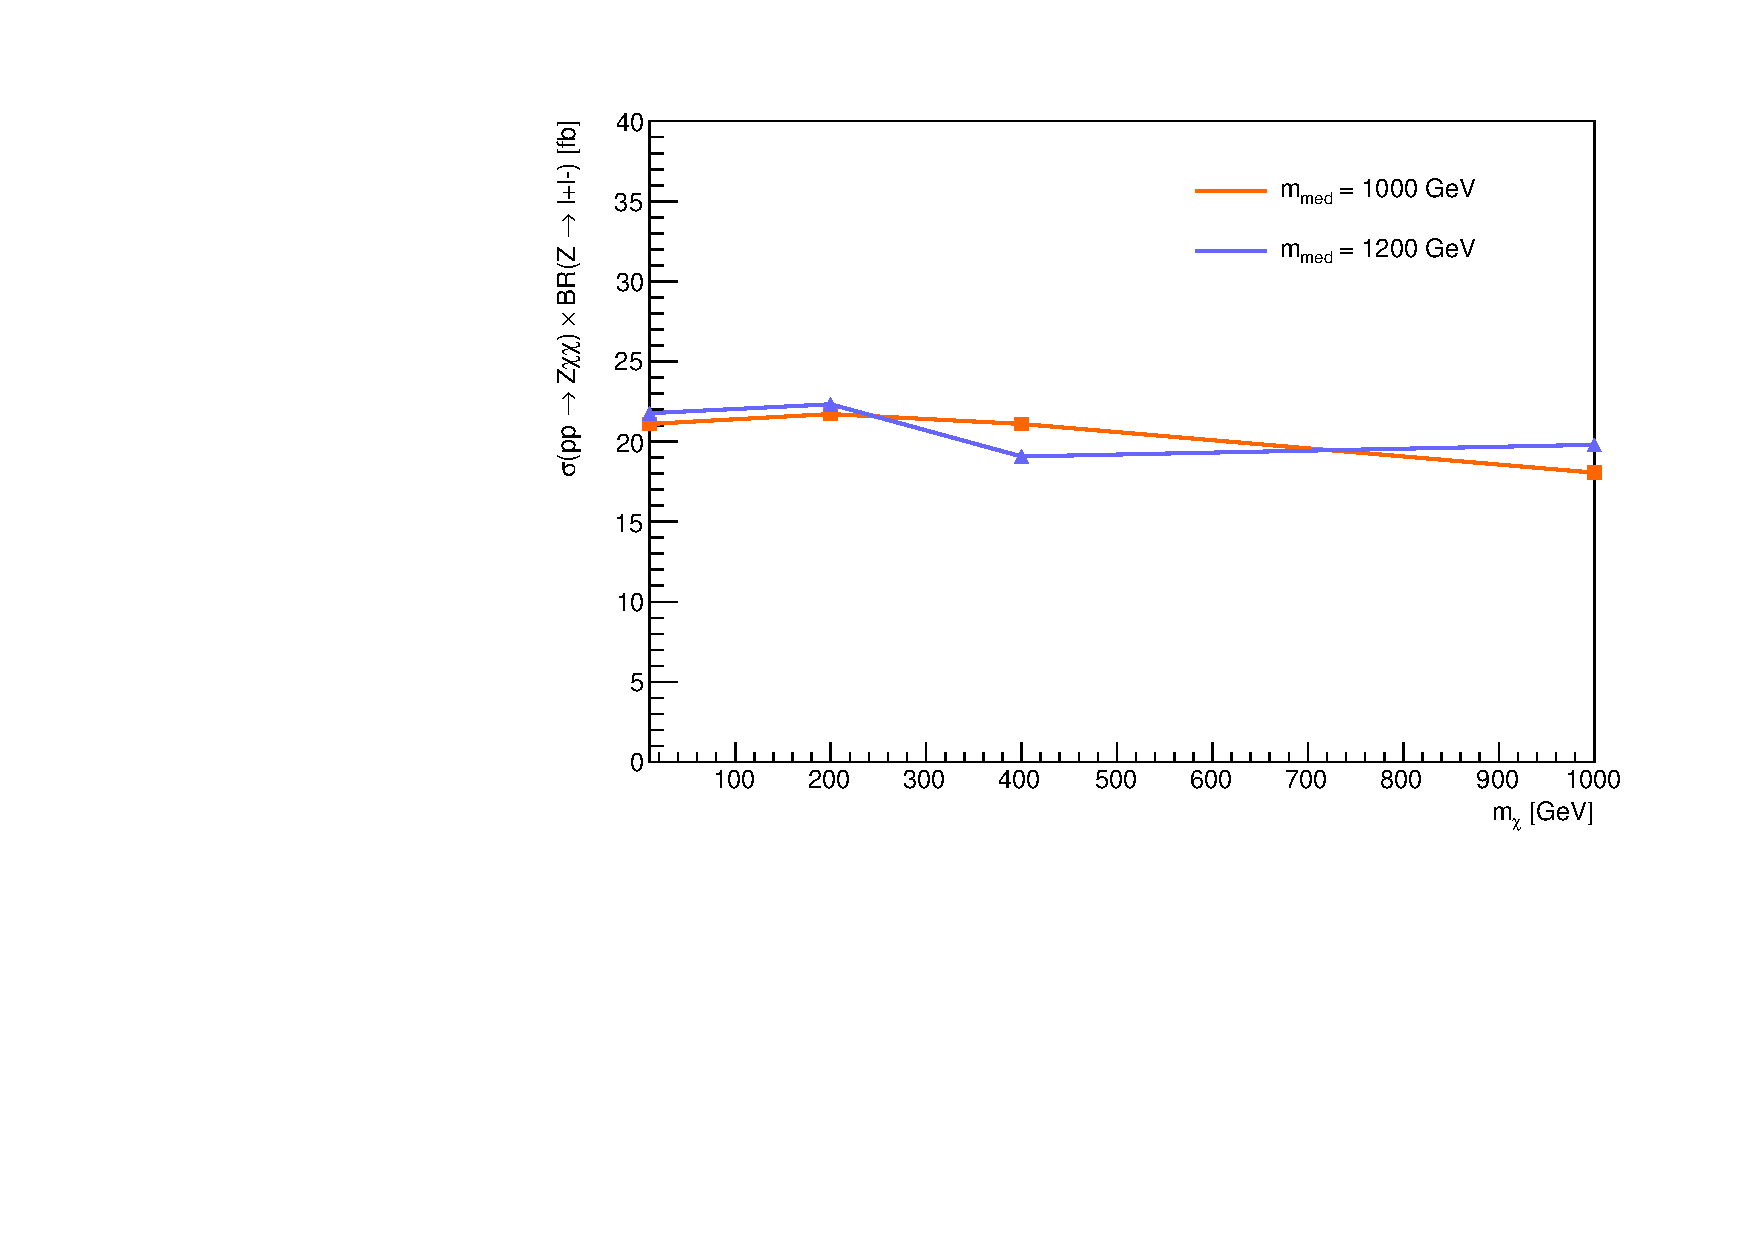
\includegraphics[width=0.45\textwidth]{figures/monoZ_sigma_limits_variedDMmass.pdf}
\caption{A very rough first plot - to be prettified! Shows the limit on sigma x BR for the sV model in the mono-Z (should be mono-jet) channel. Will change to have a band for the expected limit, and a line for the observed limit. Show 5 different coupling scenarios on one plot. Mono-Z (jet) channel, sV model.}
\label{fig:MonoZ_SVD_limit}
\end{center}
\end{figure}

\begin{figure}[!h]
\begin{center}
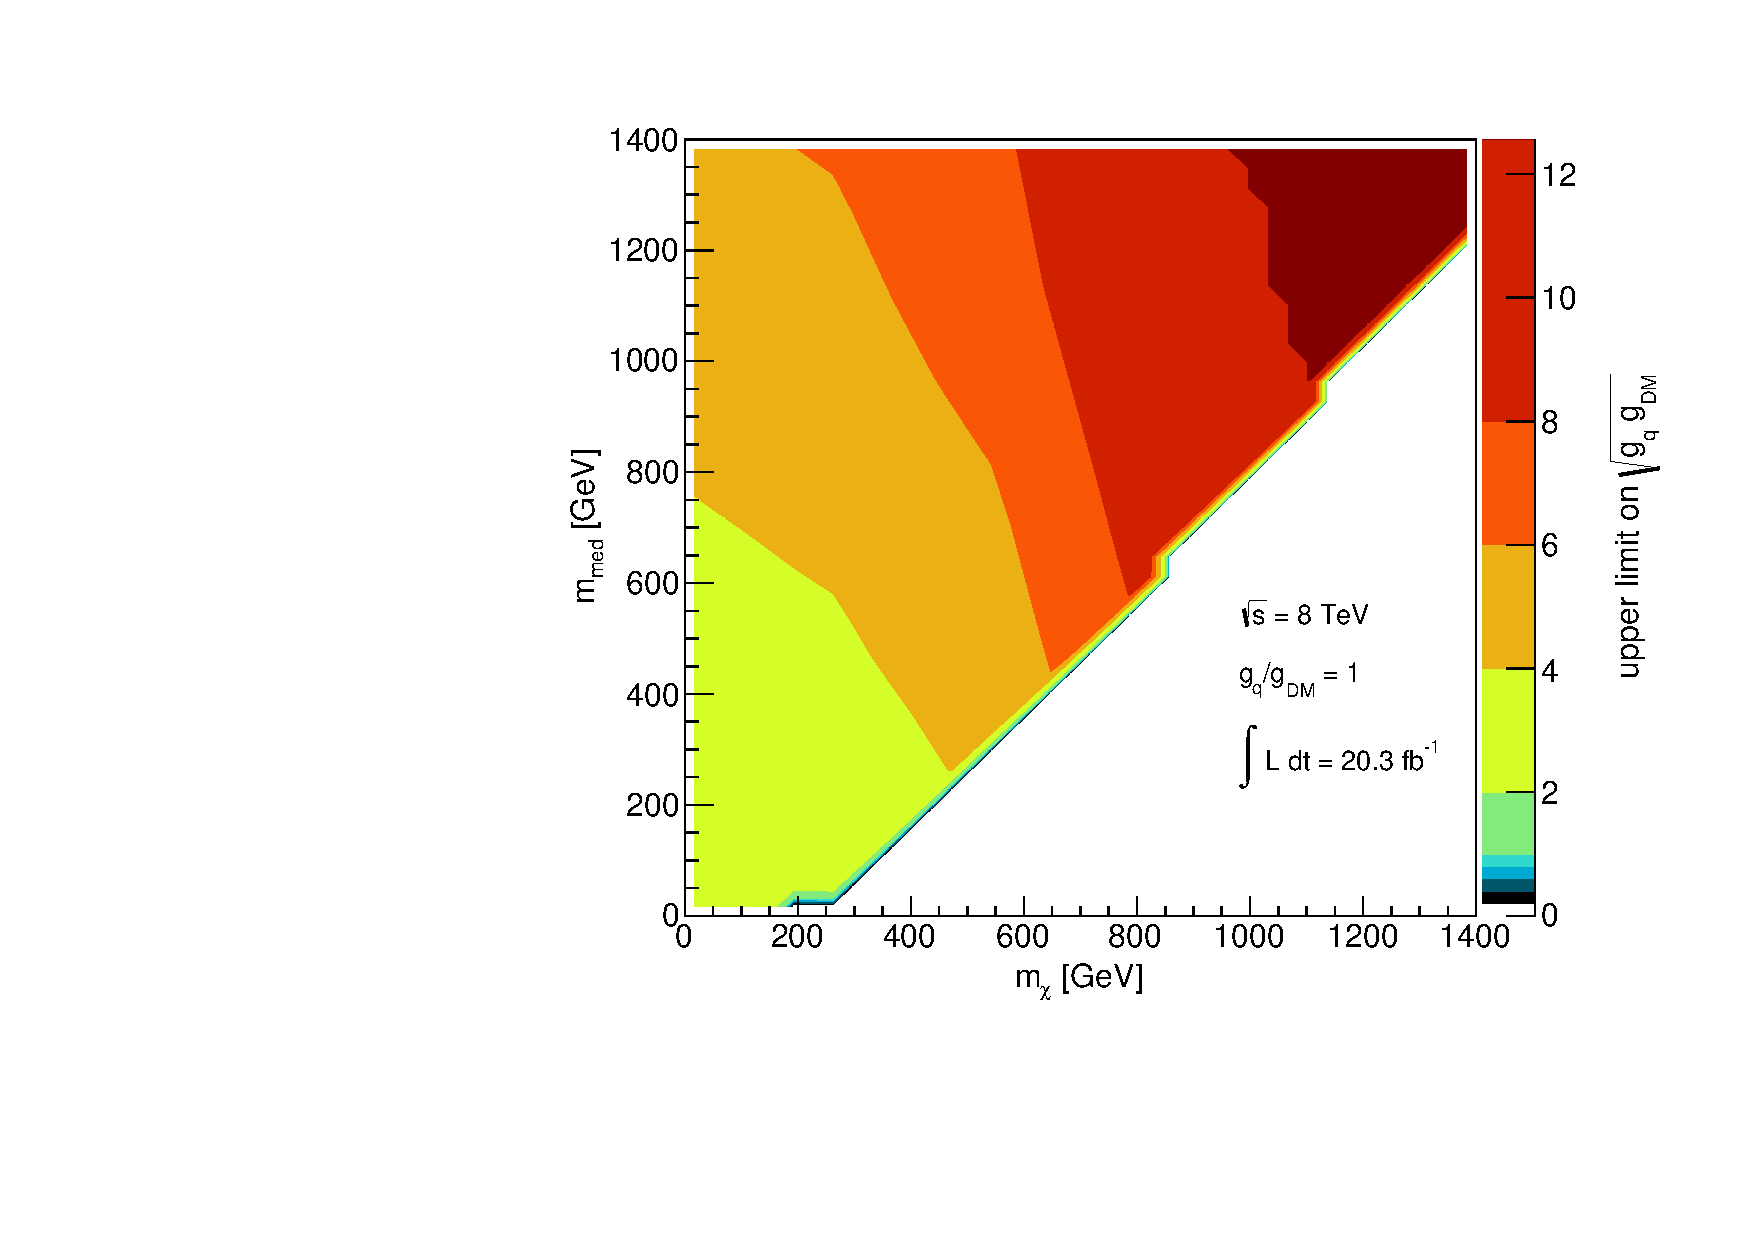
\includegraphics[width=0.45\textwidth]{figures/coupling_limits_TSD_1.pdf}
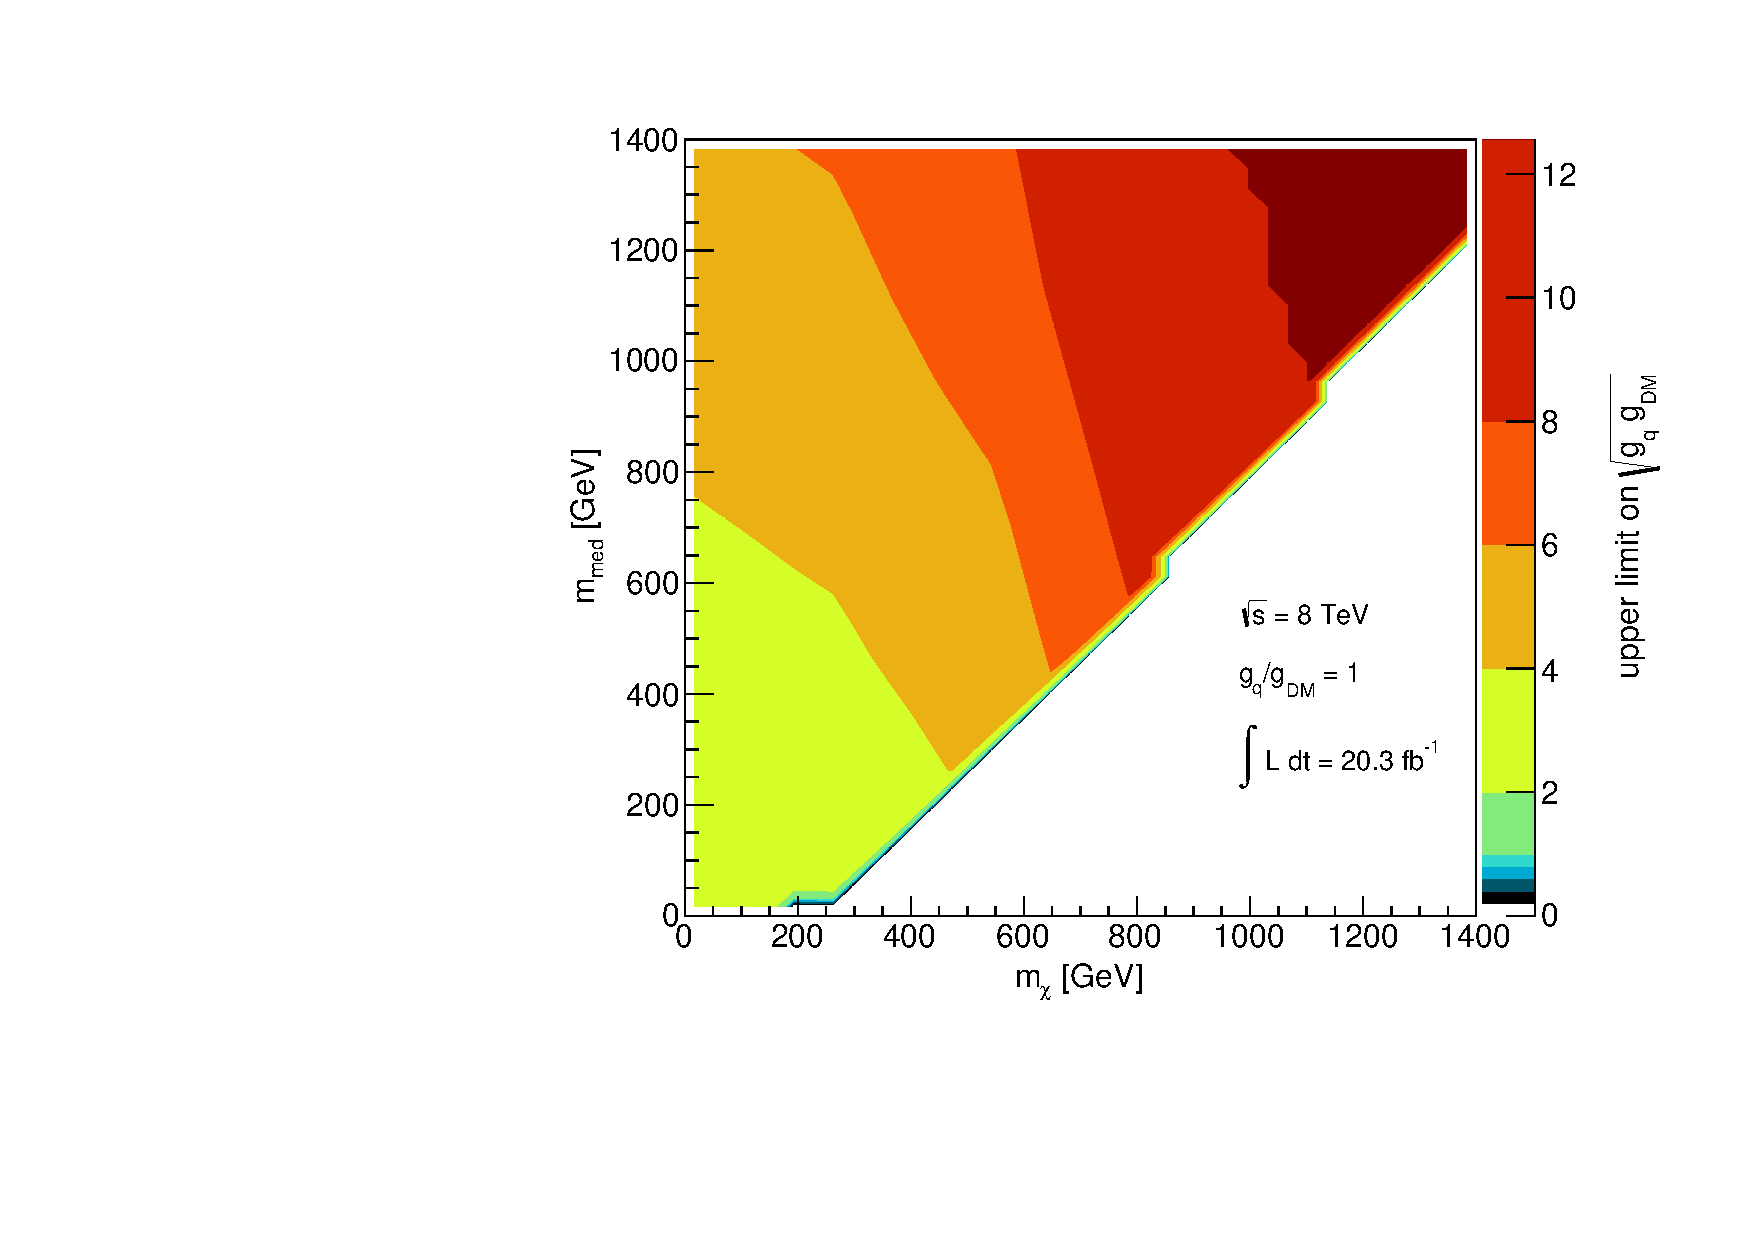
\includegraphics[width=0.45\textwidth]{figures/coupling_limits_TSD_1.pdf}
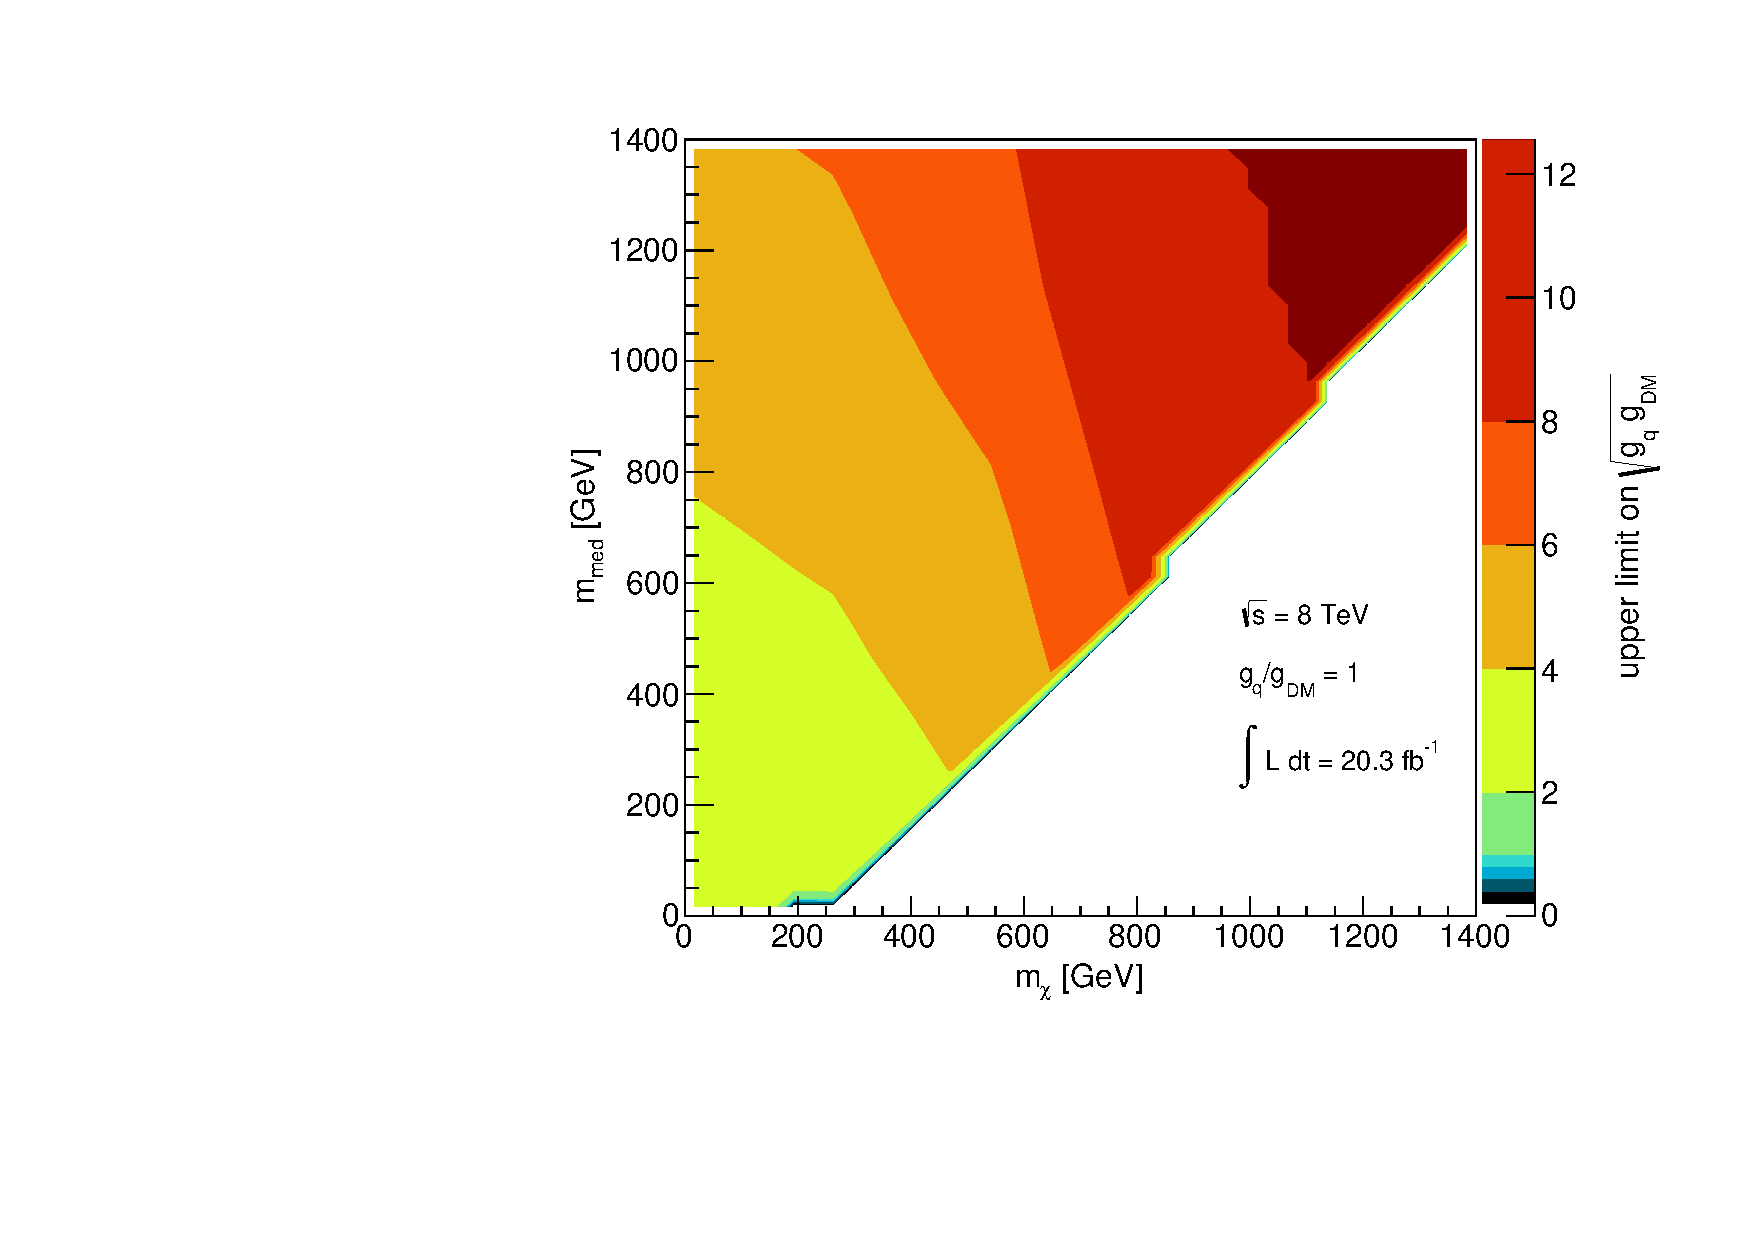
\includegraphics[width=0.45\textwidth]{figures/coupling_limits_TSD_1.pdf}
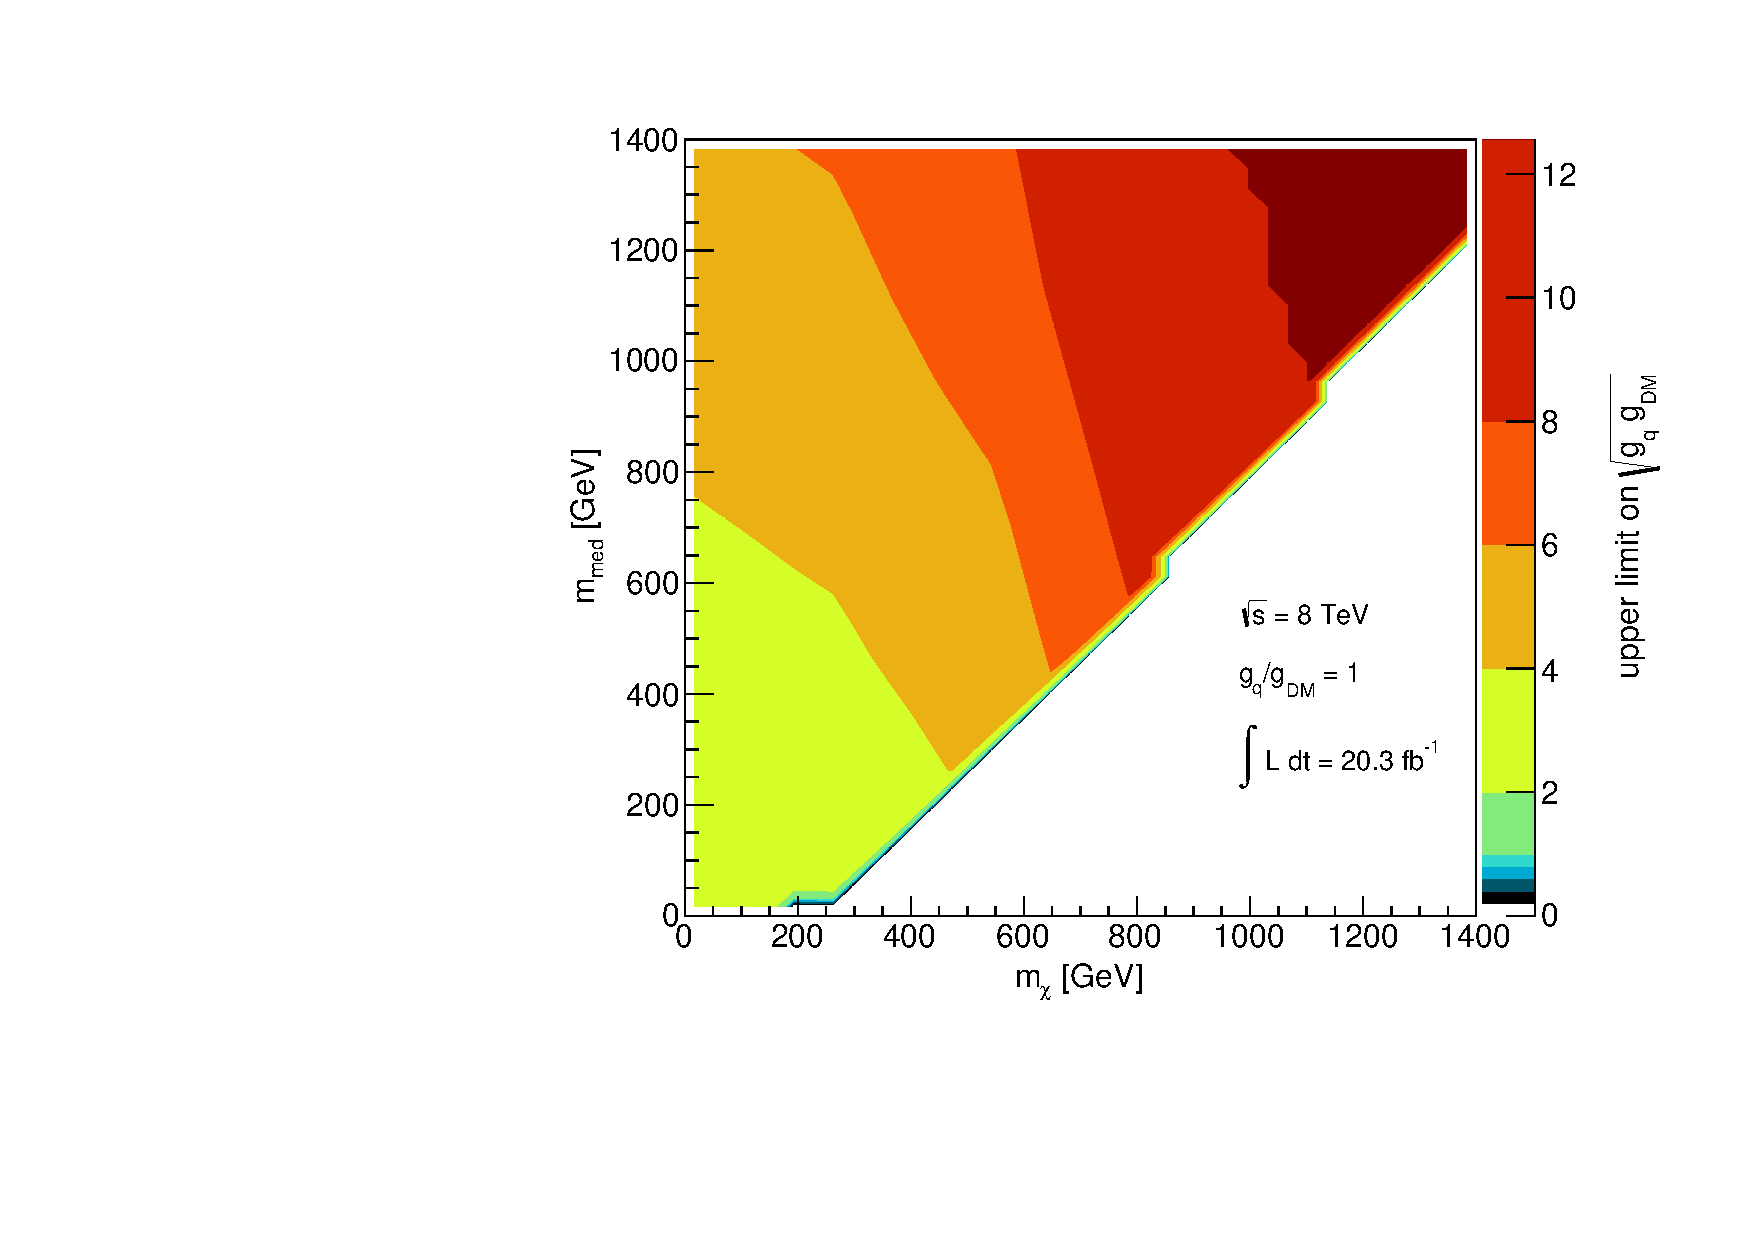
\includegraphics[width=0.45\textwidth]{figures/coupling_limits_TSD_1.pdf}
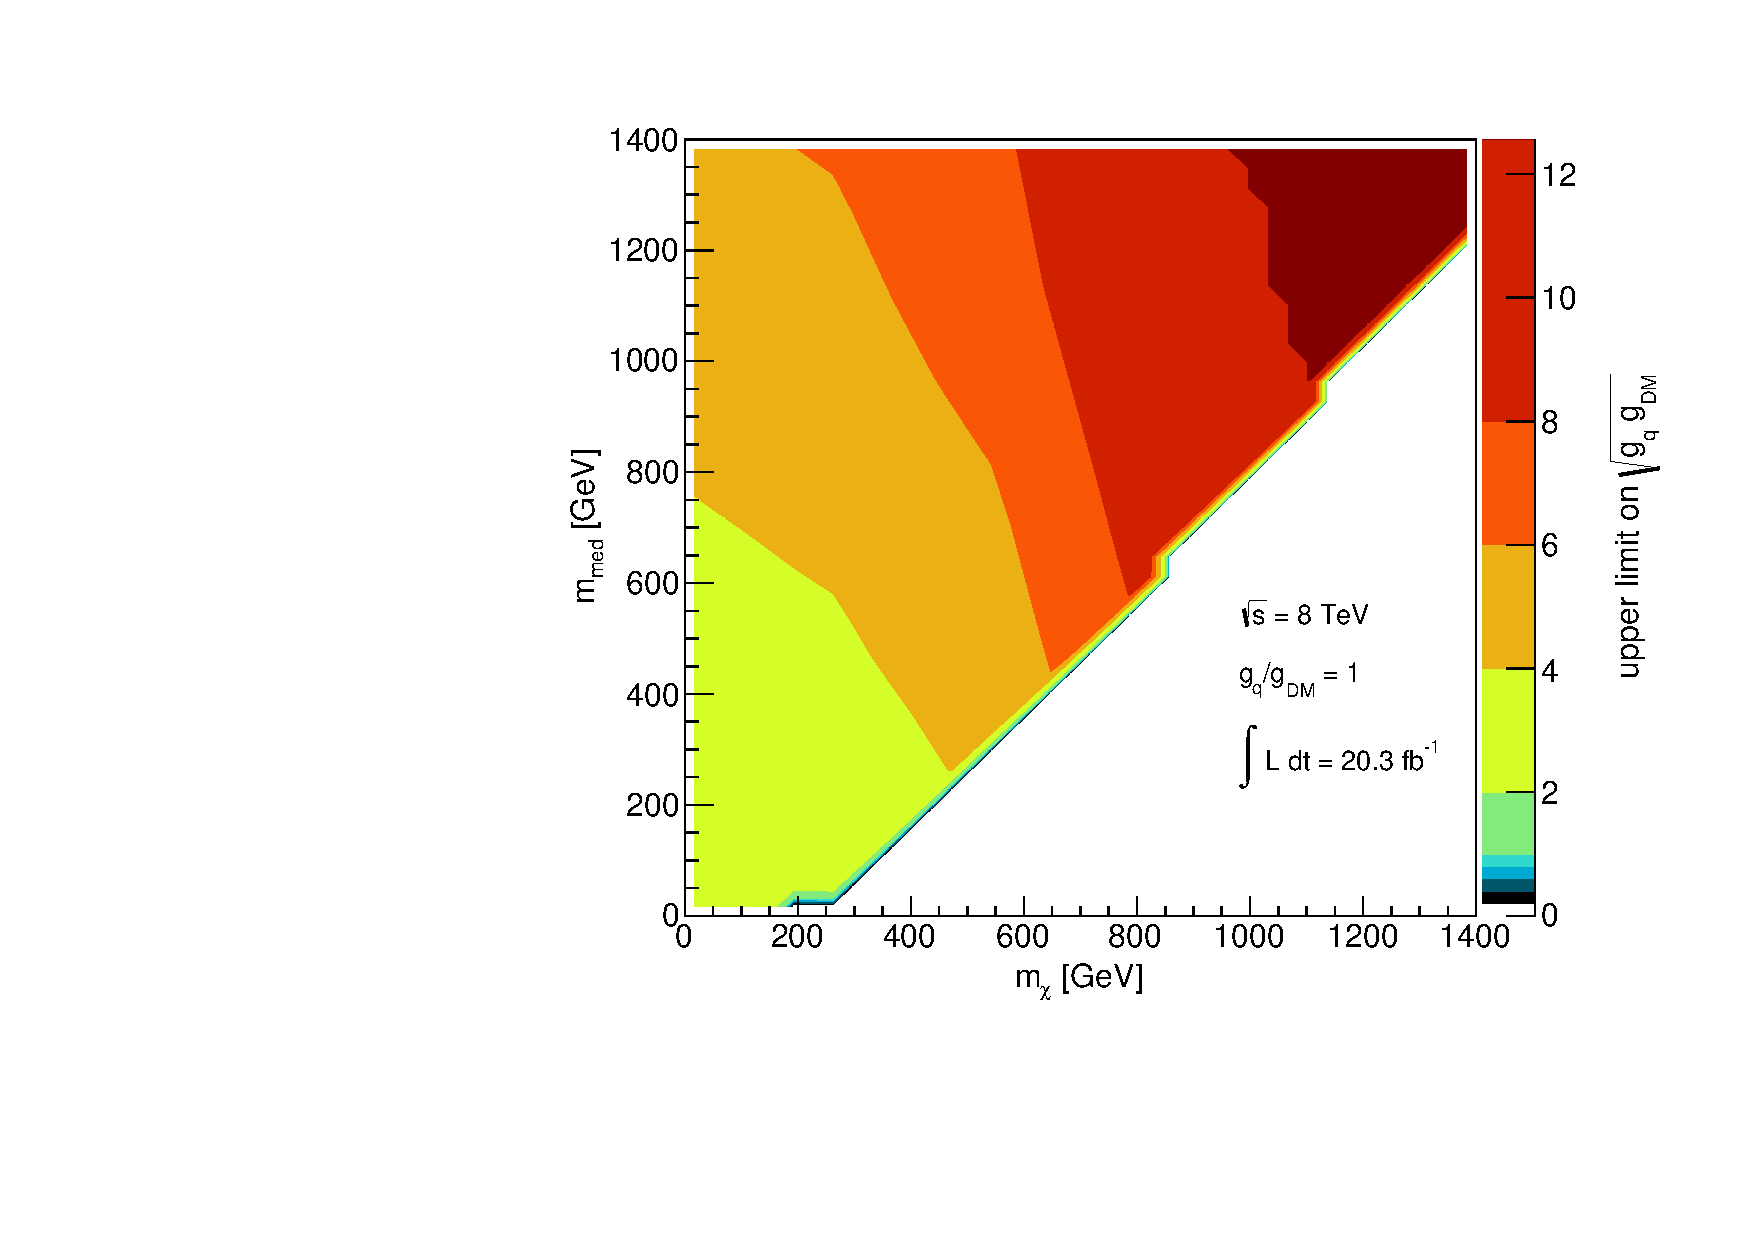
\includegraphics[width=0.45\textwidth]{figures/coupling_limits_TSD_1.pdf}
\caption{Limit on coupling strength for the sV model, in the mono-Z (should be jet) channel.  Need to fix up the scale on the z-axis and include mass points as dots on the plot. To be replaced with 5 plots with different coupling ratios, gq/gchi = 0.2, 0.5, 1, 2, 5. REPLACE WITH SV MODEL PLOTS.}
\label{fig:Monojet_SVD_couplinglimit}
\end{center}
\end{figure}

\begin{figure}[!h]
\begin{center}
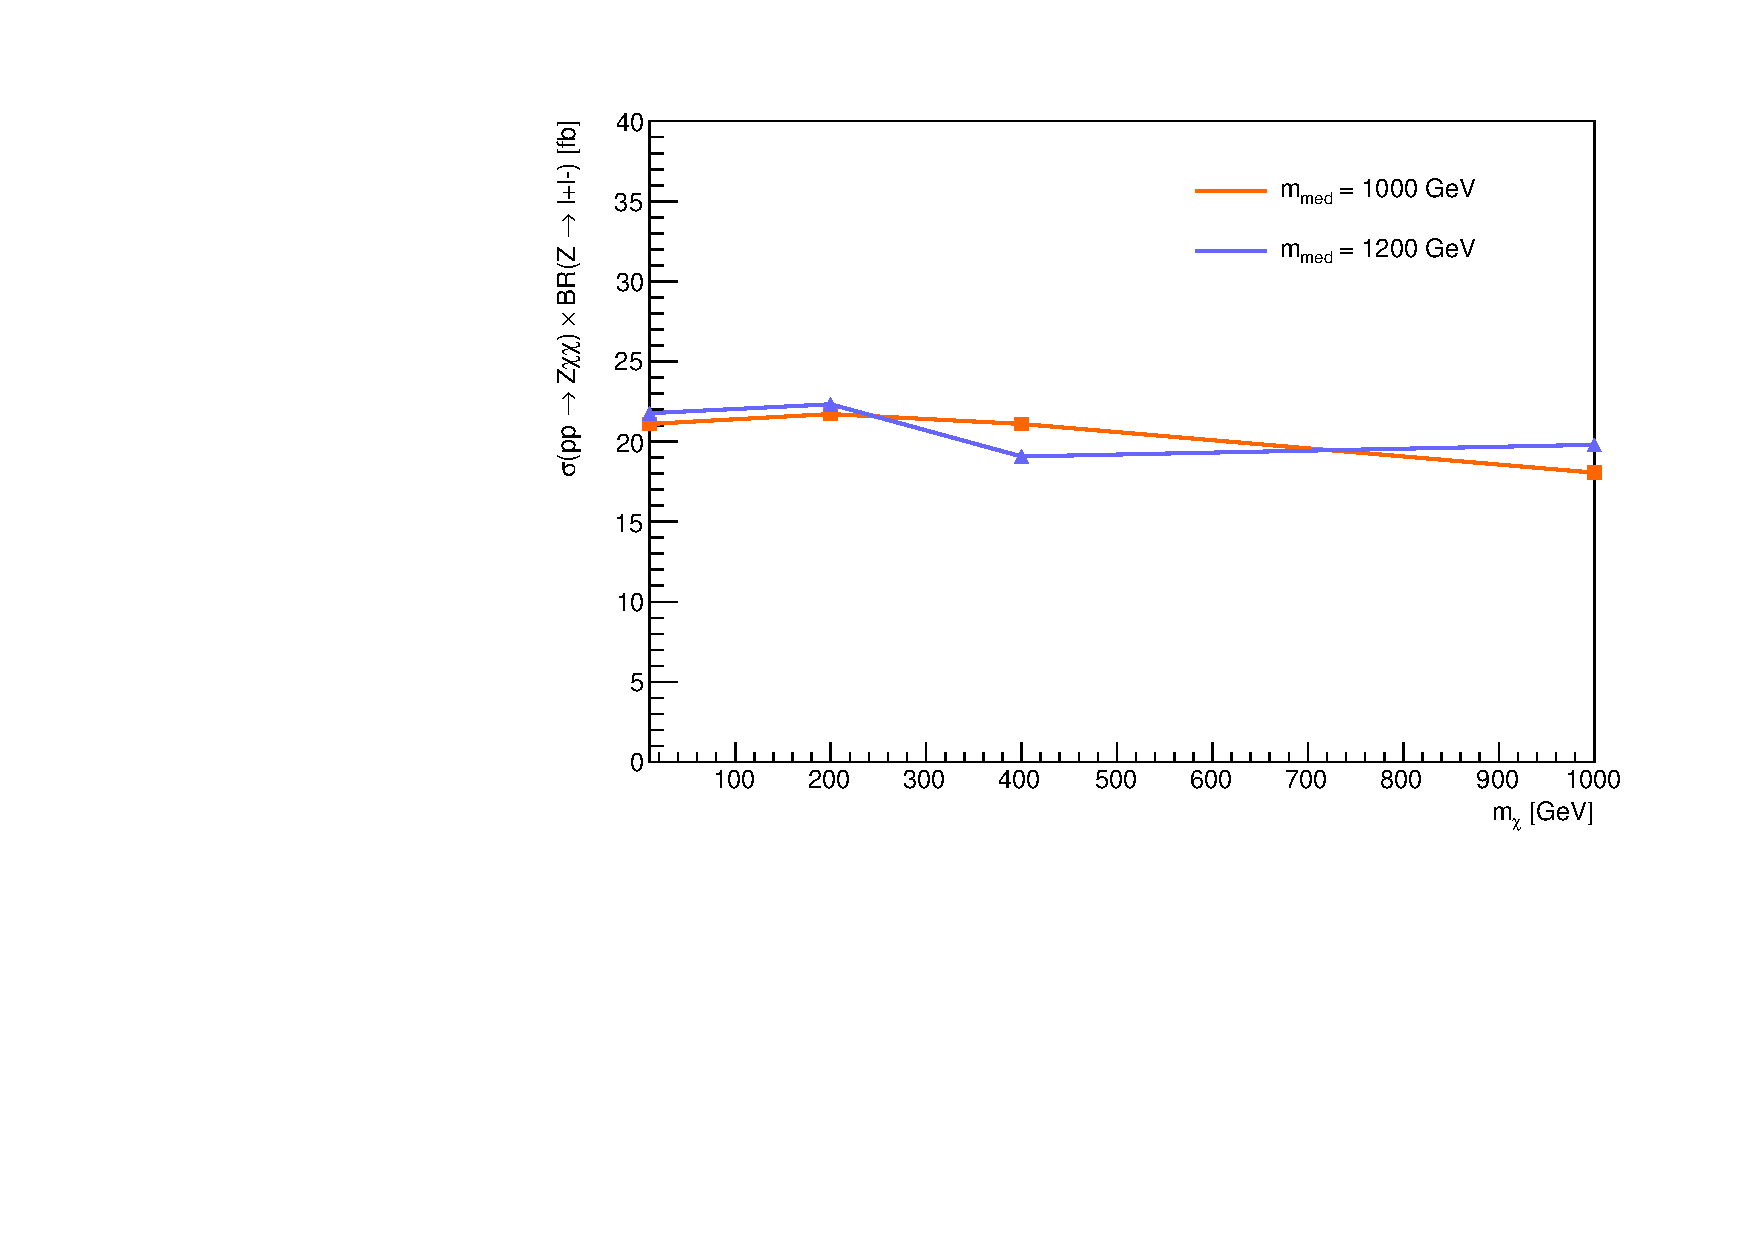
\includegraphics[width=0.45\textwidth]{figures/monoZ_sigma_limits_variedDMmass.pdf}
\caption{Mono-jet channel, sS model. REPLACE WITH SS MODEL PLOTS.}
\label{fig:Monojet_SSD_limit}
\end{center}
\end{figure}

\begin{figure}[!h]
\begin{center}
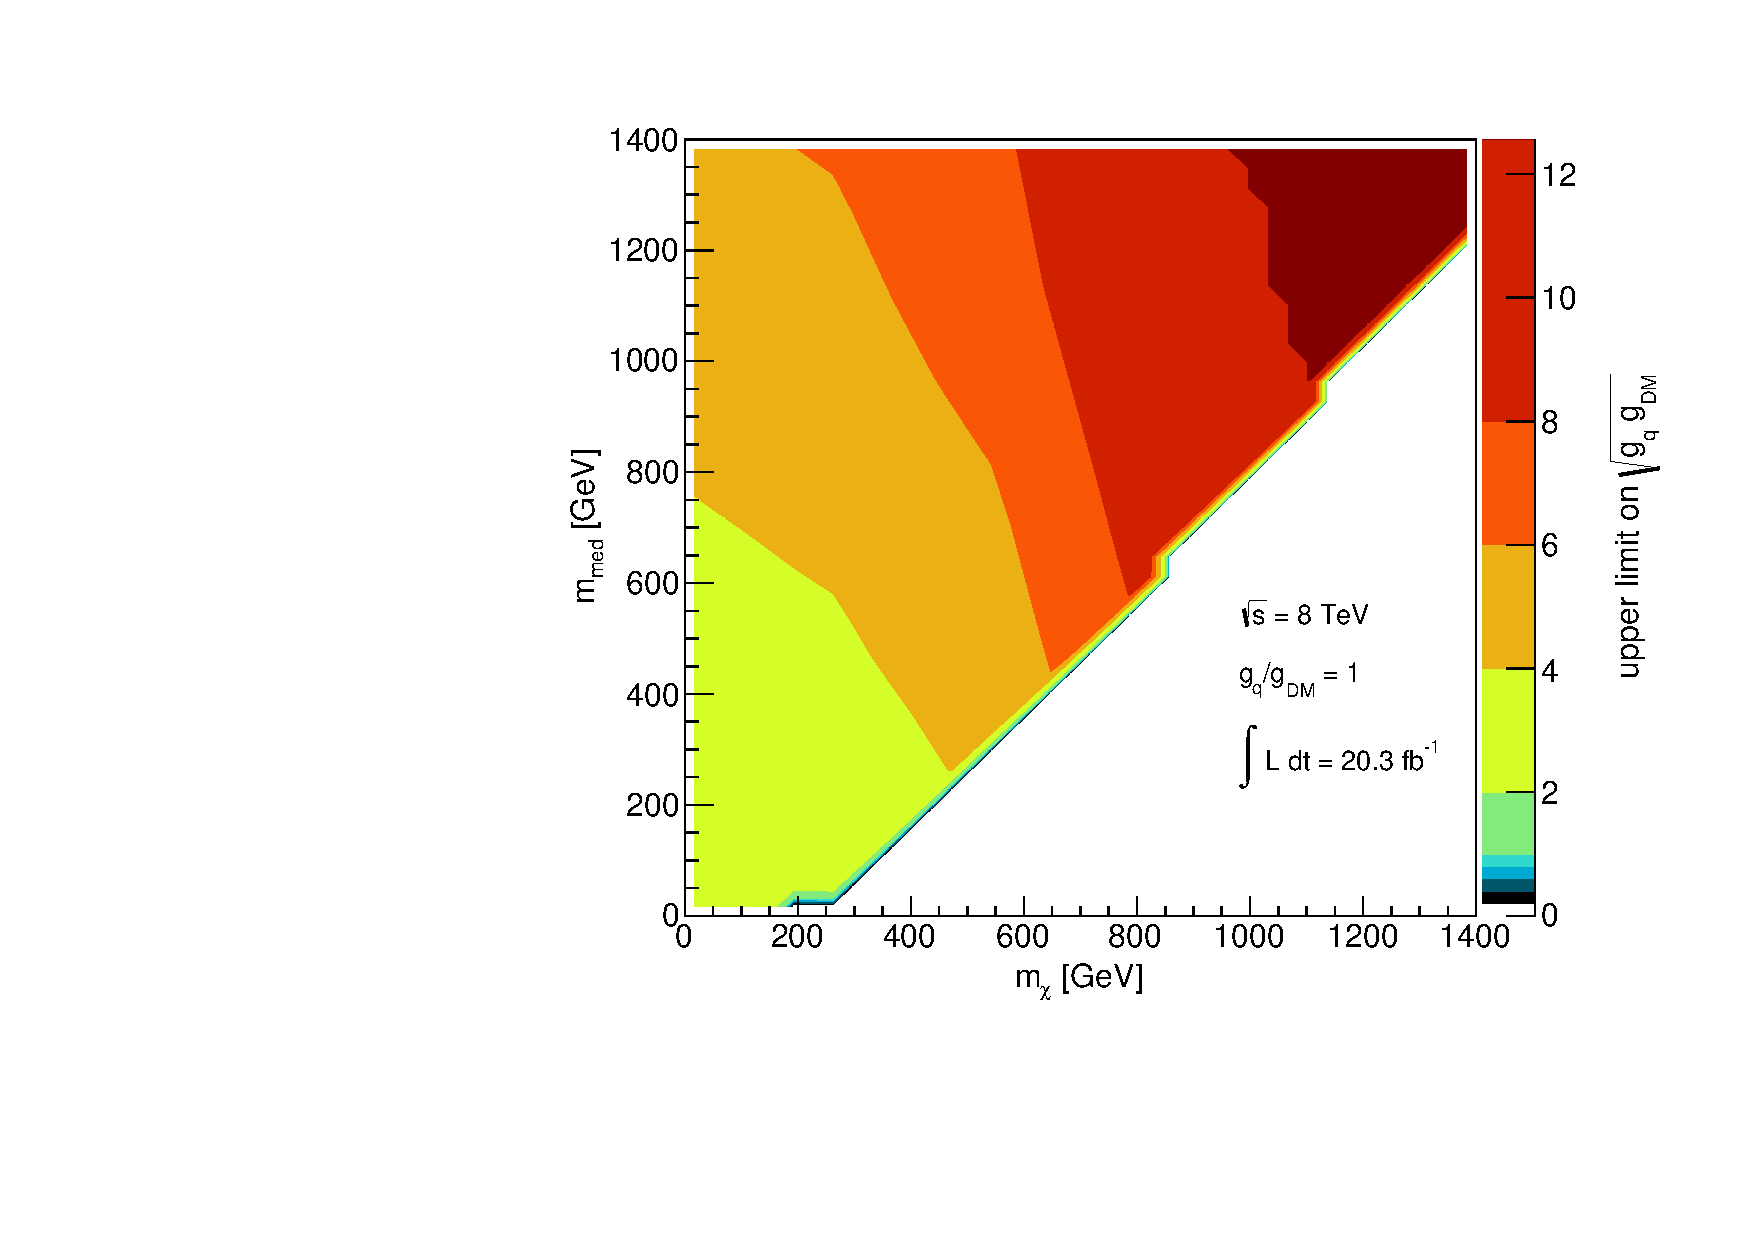
\includegraphics[width=0.45\textwidth]{figures/coupling_limits_TSD_1.pdf}
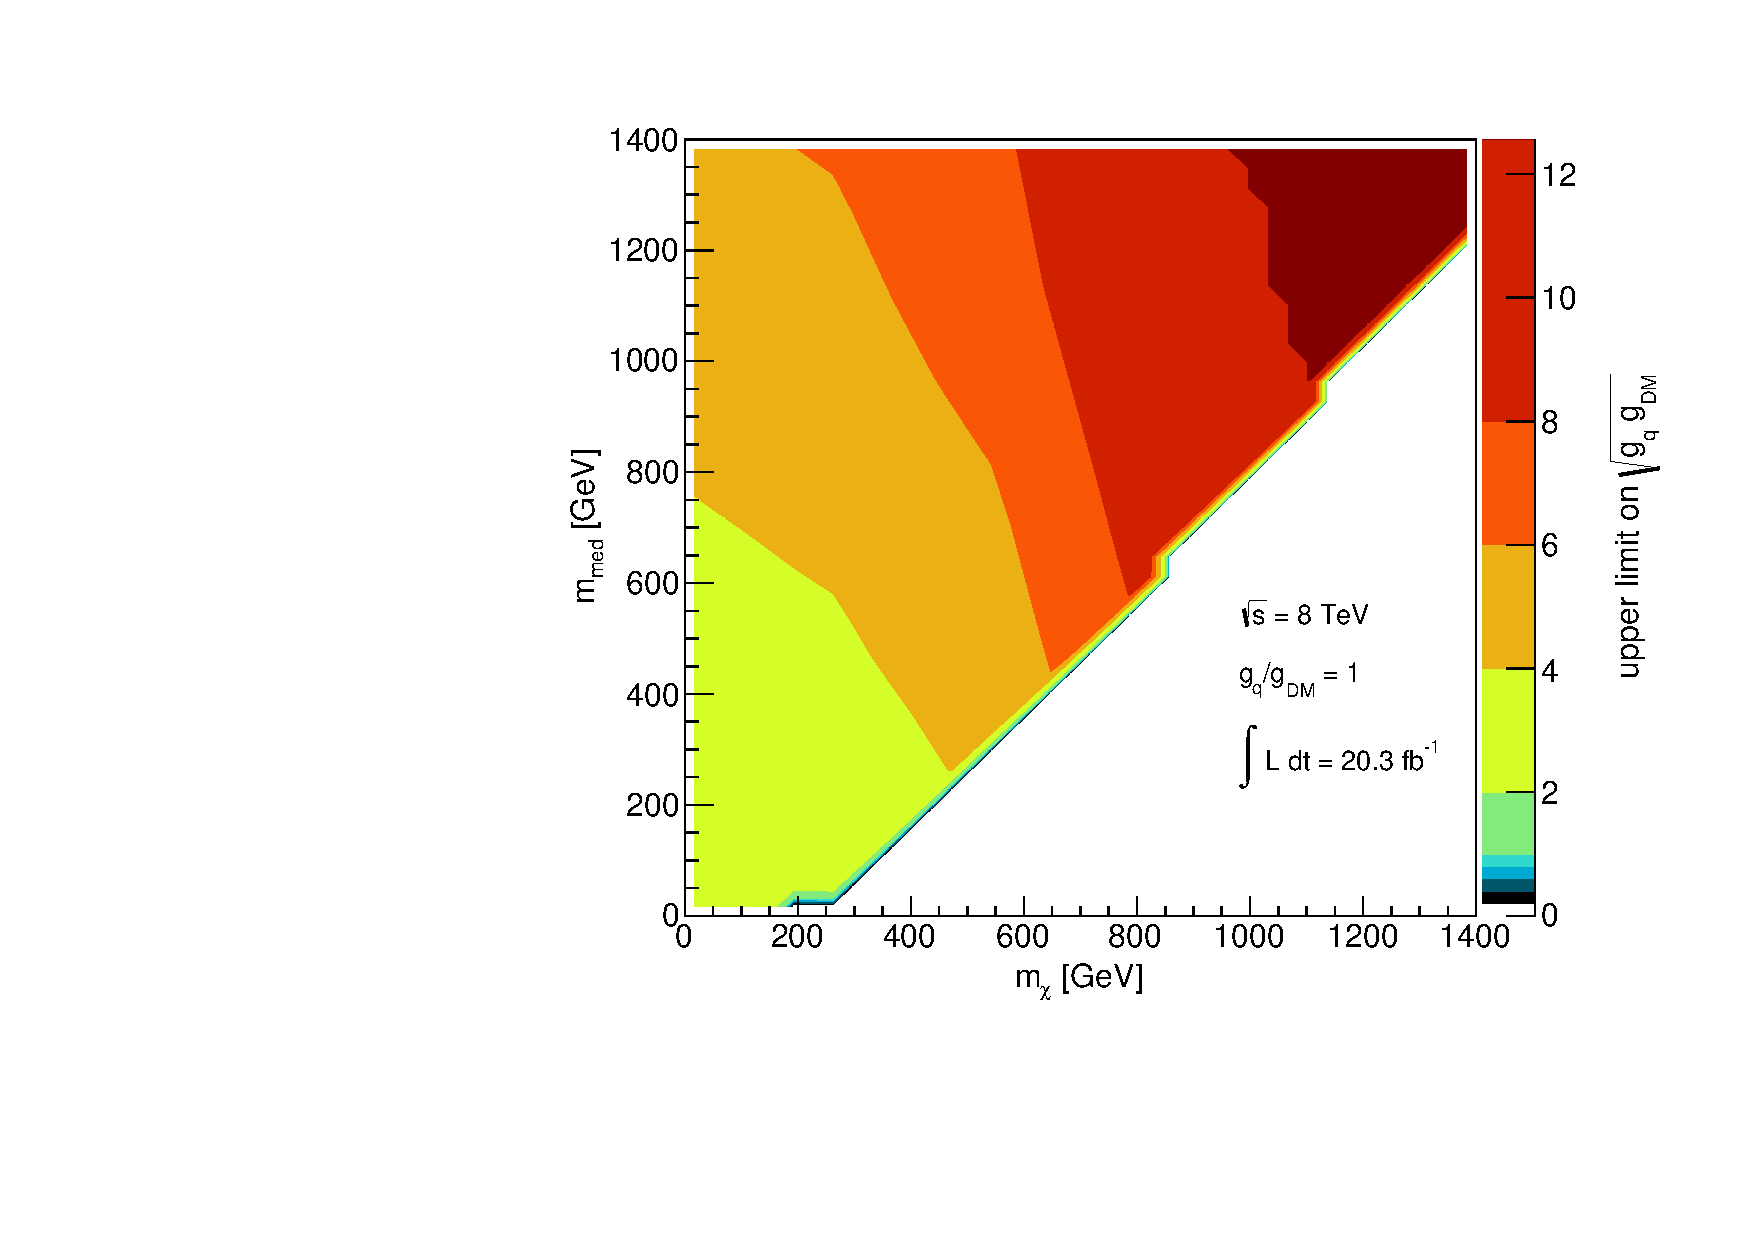
\includegraphics[width=0.45\textwidth]{figures/coupling_limits_TSD_1.pdf}
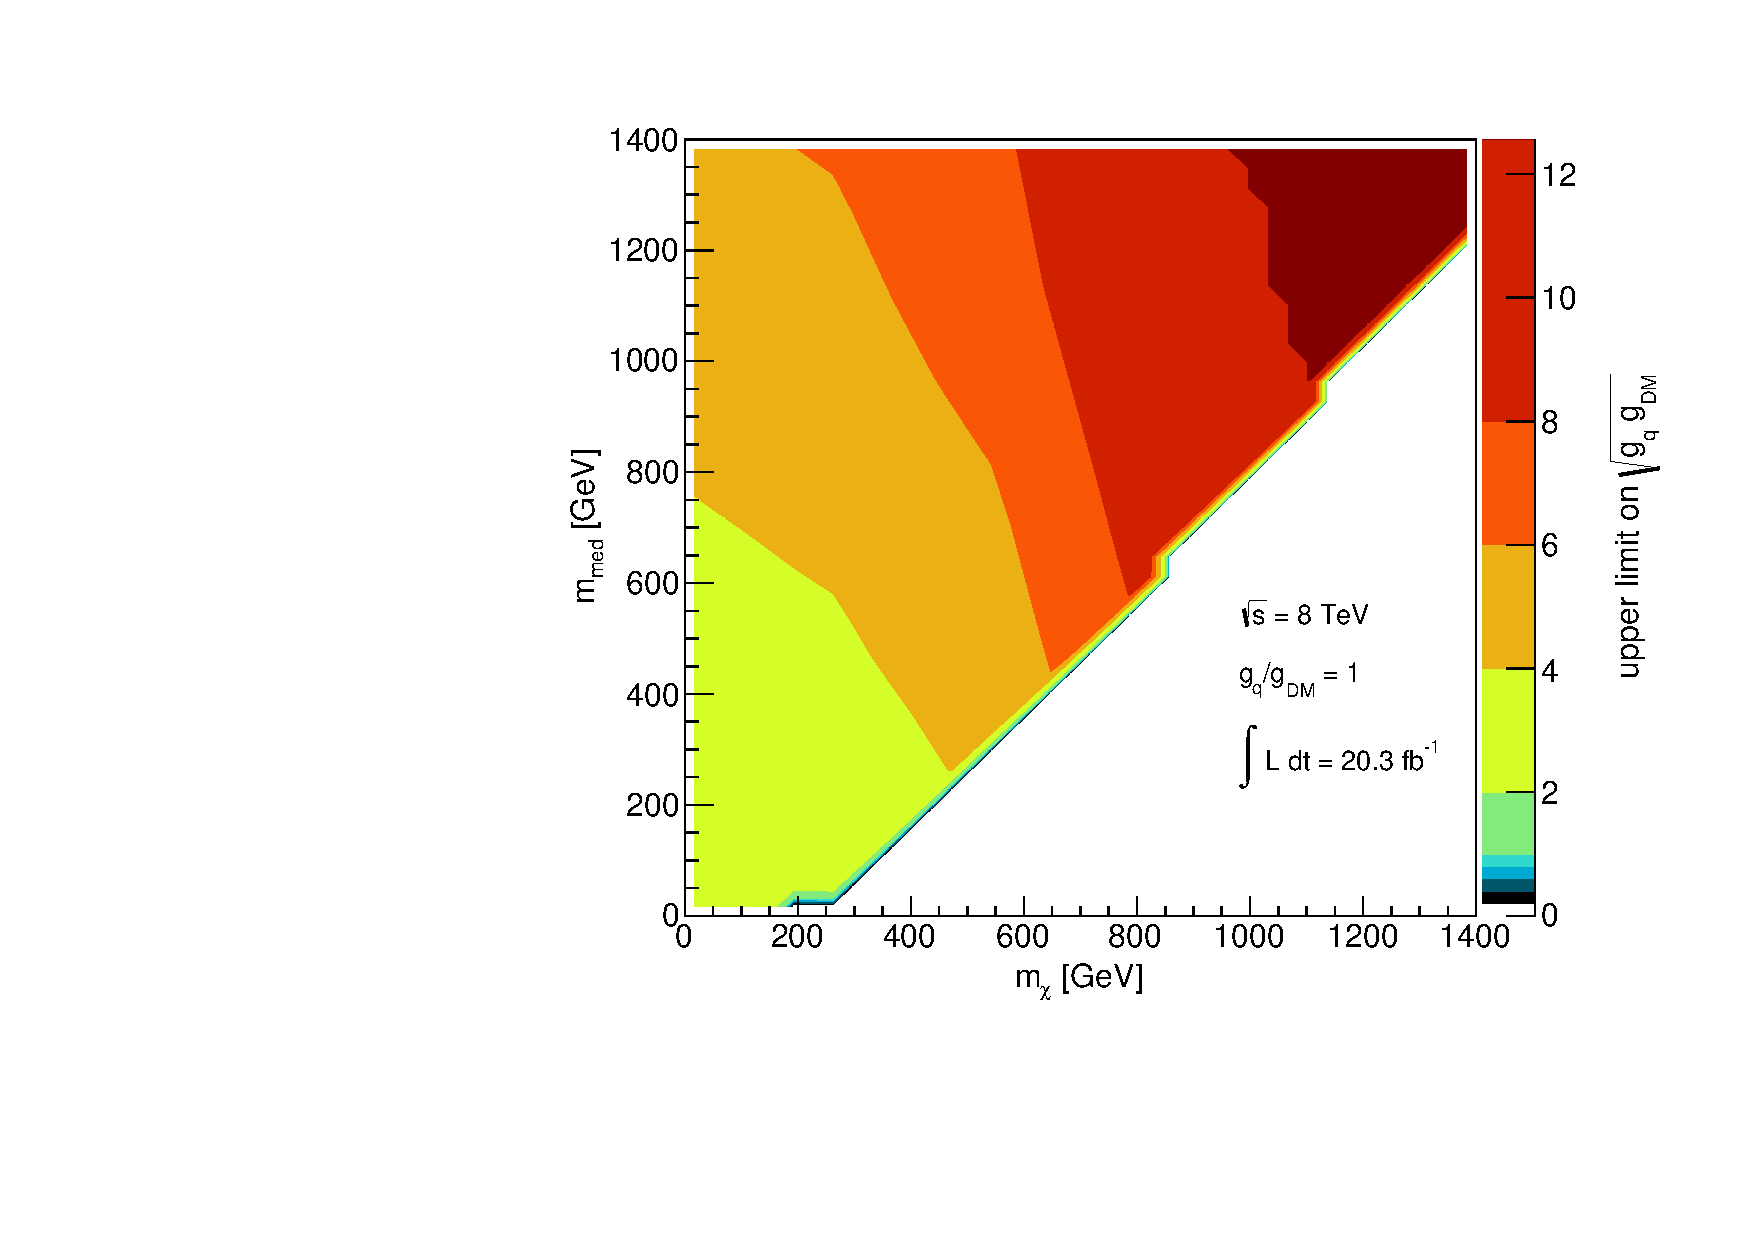
\includegraphics[width=0.45\textwidth]{figures/coupling_limits_TSD_1.pdf}
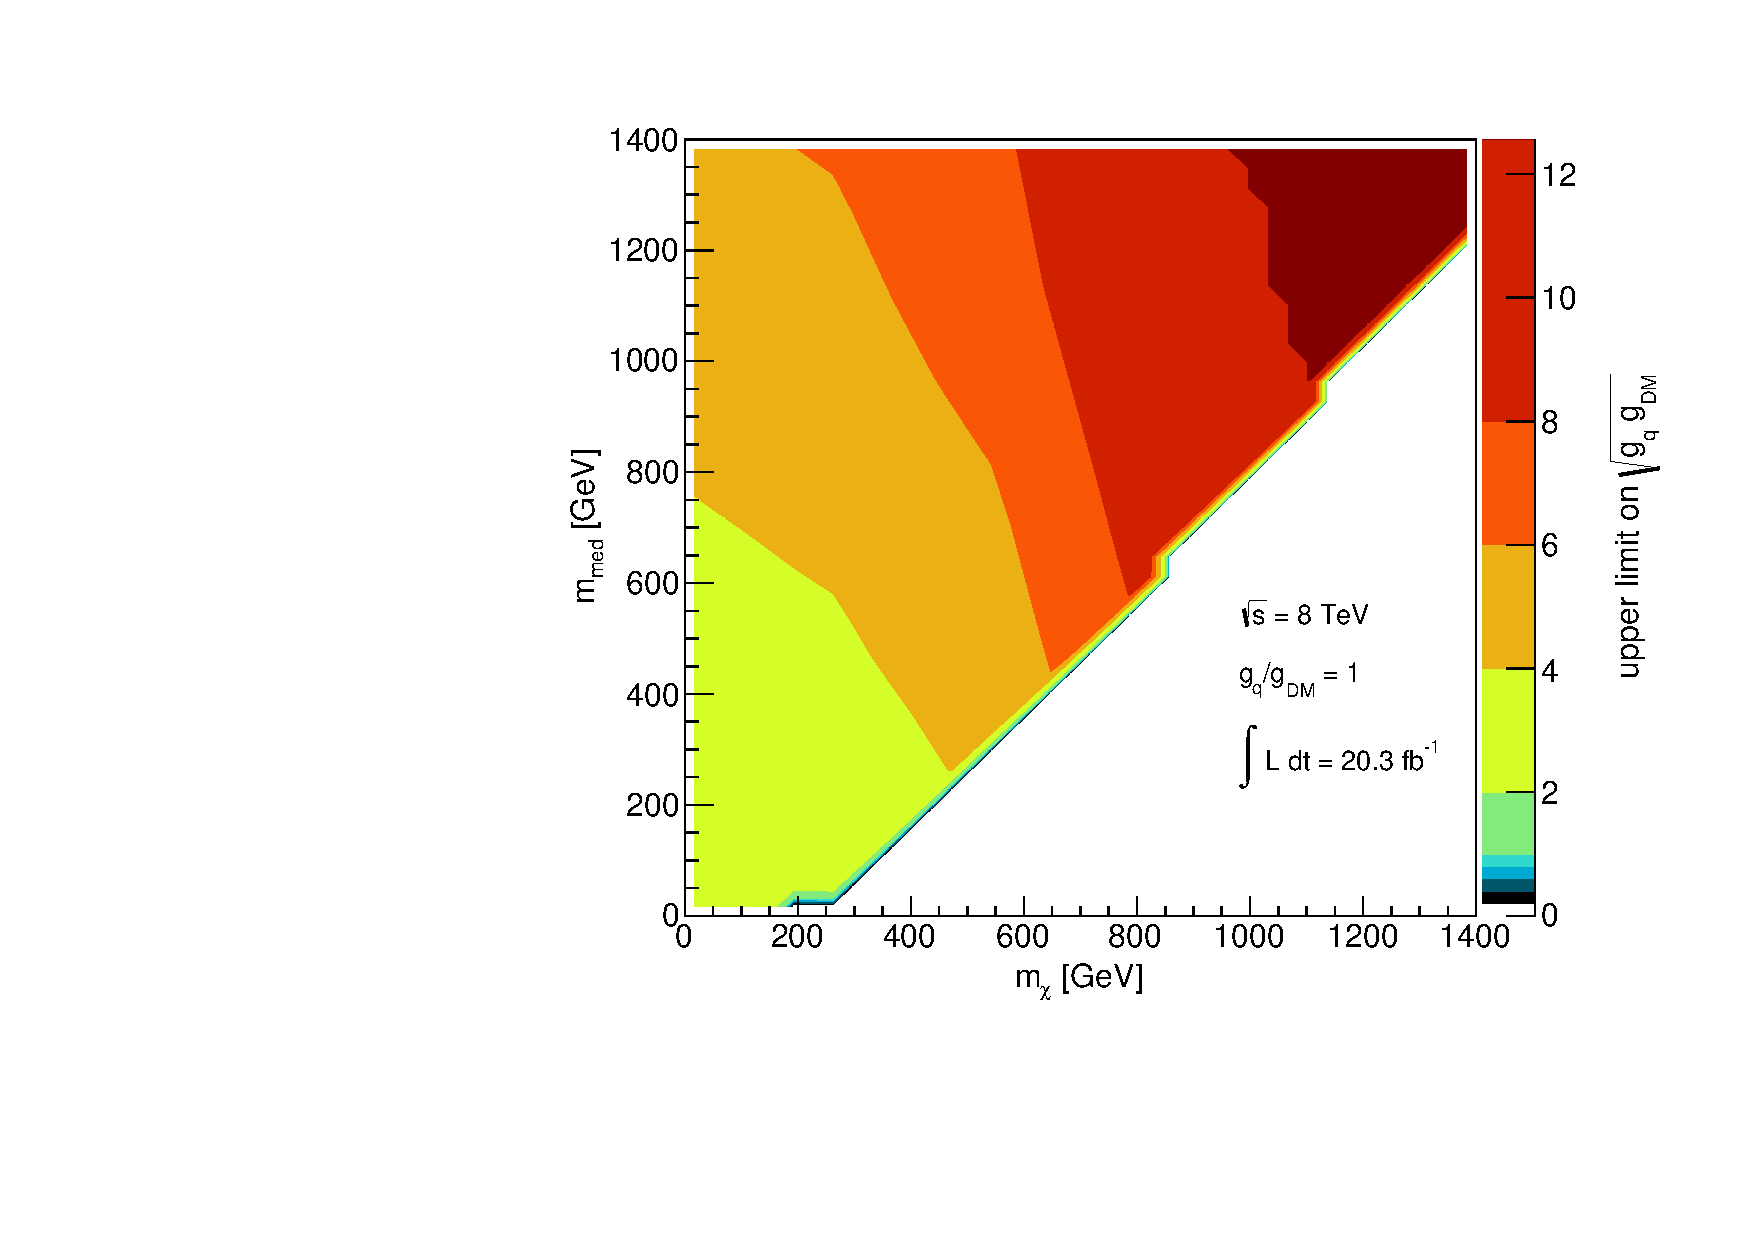
\includegraphics[width=0.45\textwidth]{figures/coupling_limits_TSD_1.pdf}
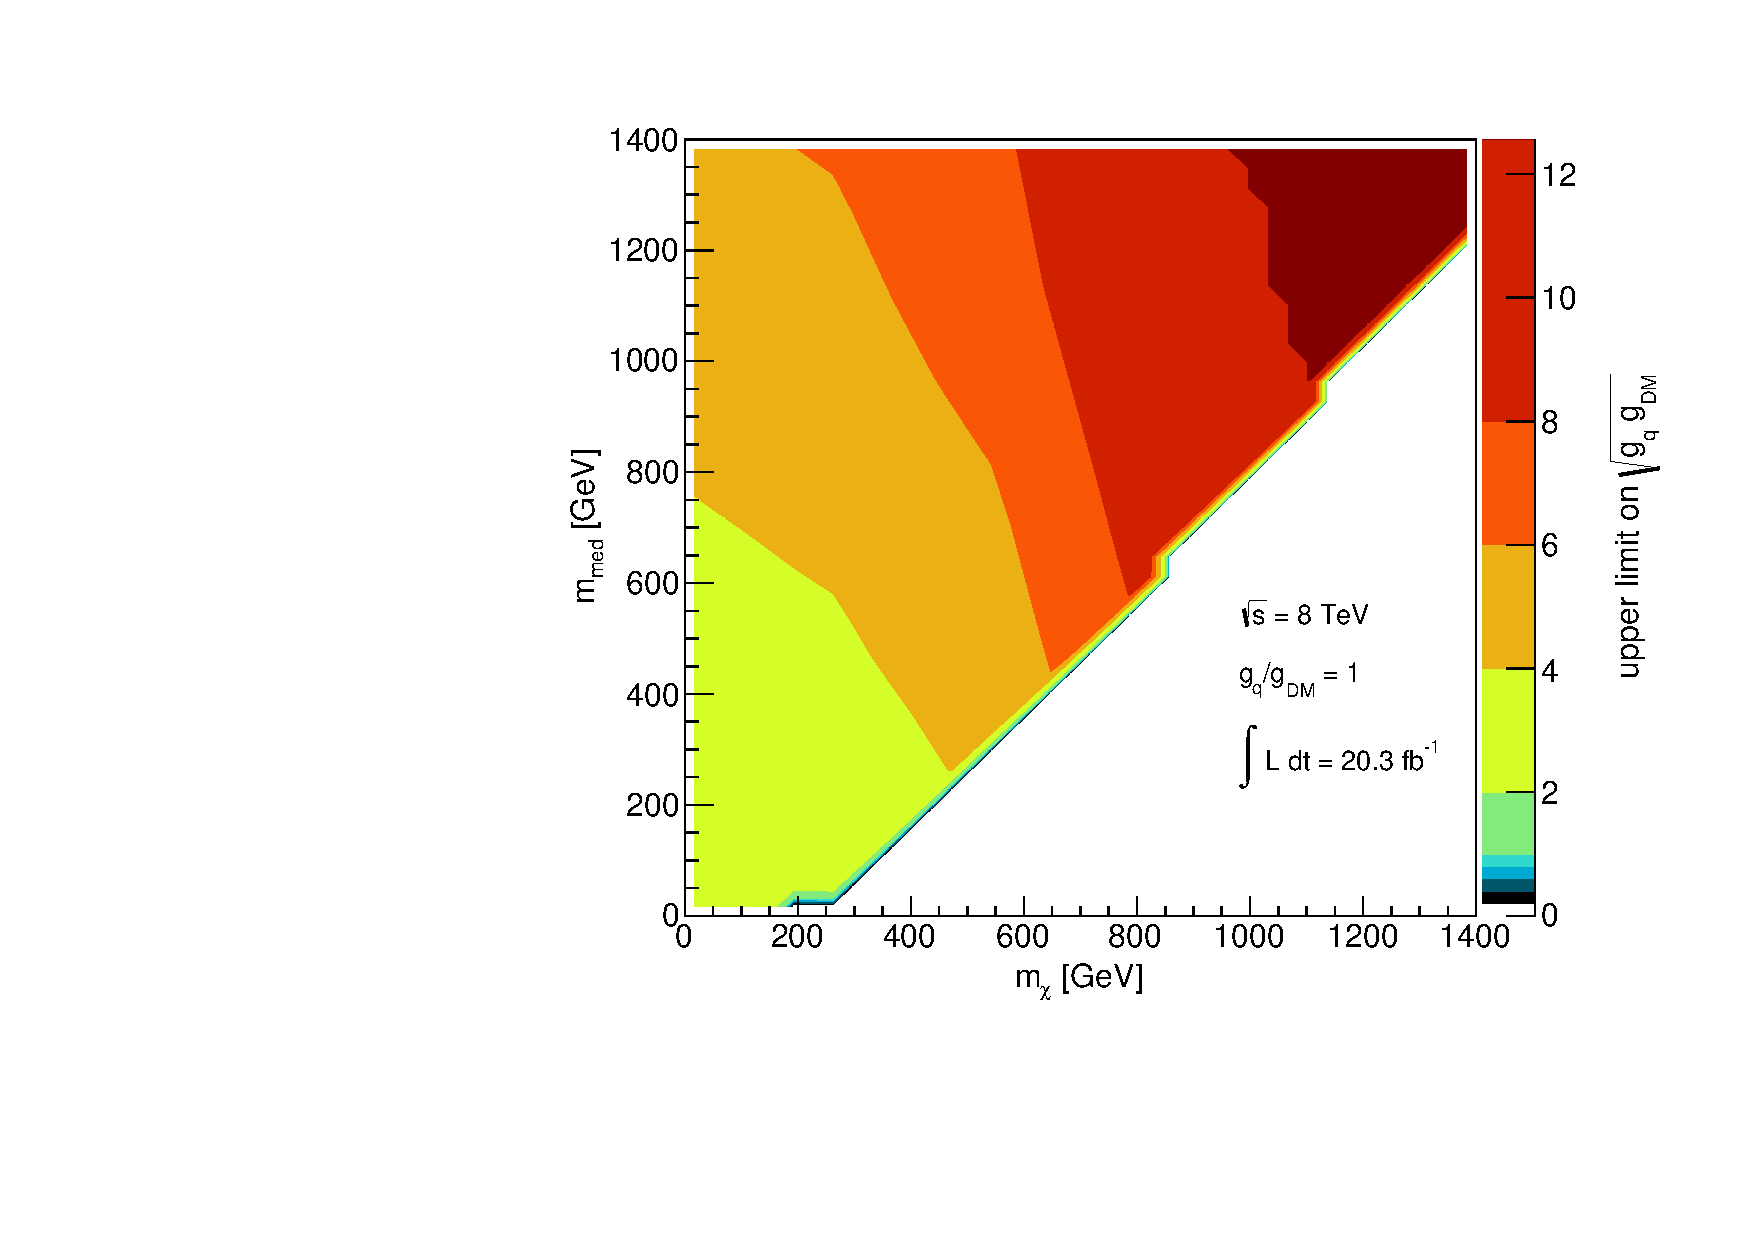
\includegraphics[width=0.45\textwidth]{figures/coupling_limits_TSD_1.pdf}
\caption{sS model coupling limit. REPLACE WITH SS MODEL PLOTS.}
\label{fig:Monojet_SSD_couplinglimit}
\end{center}
\end{figure}

\begin{figure}[!h]
\begin{center}
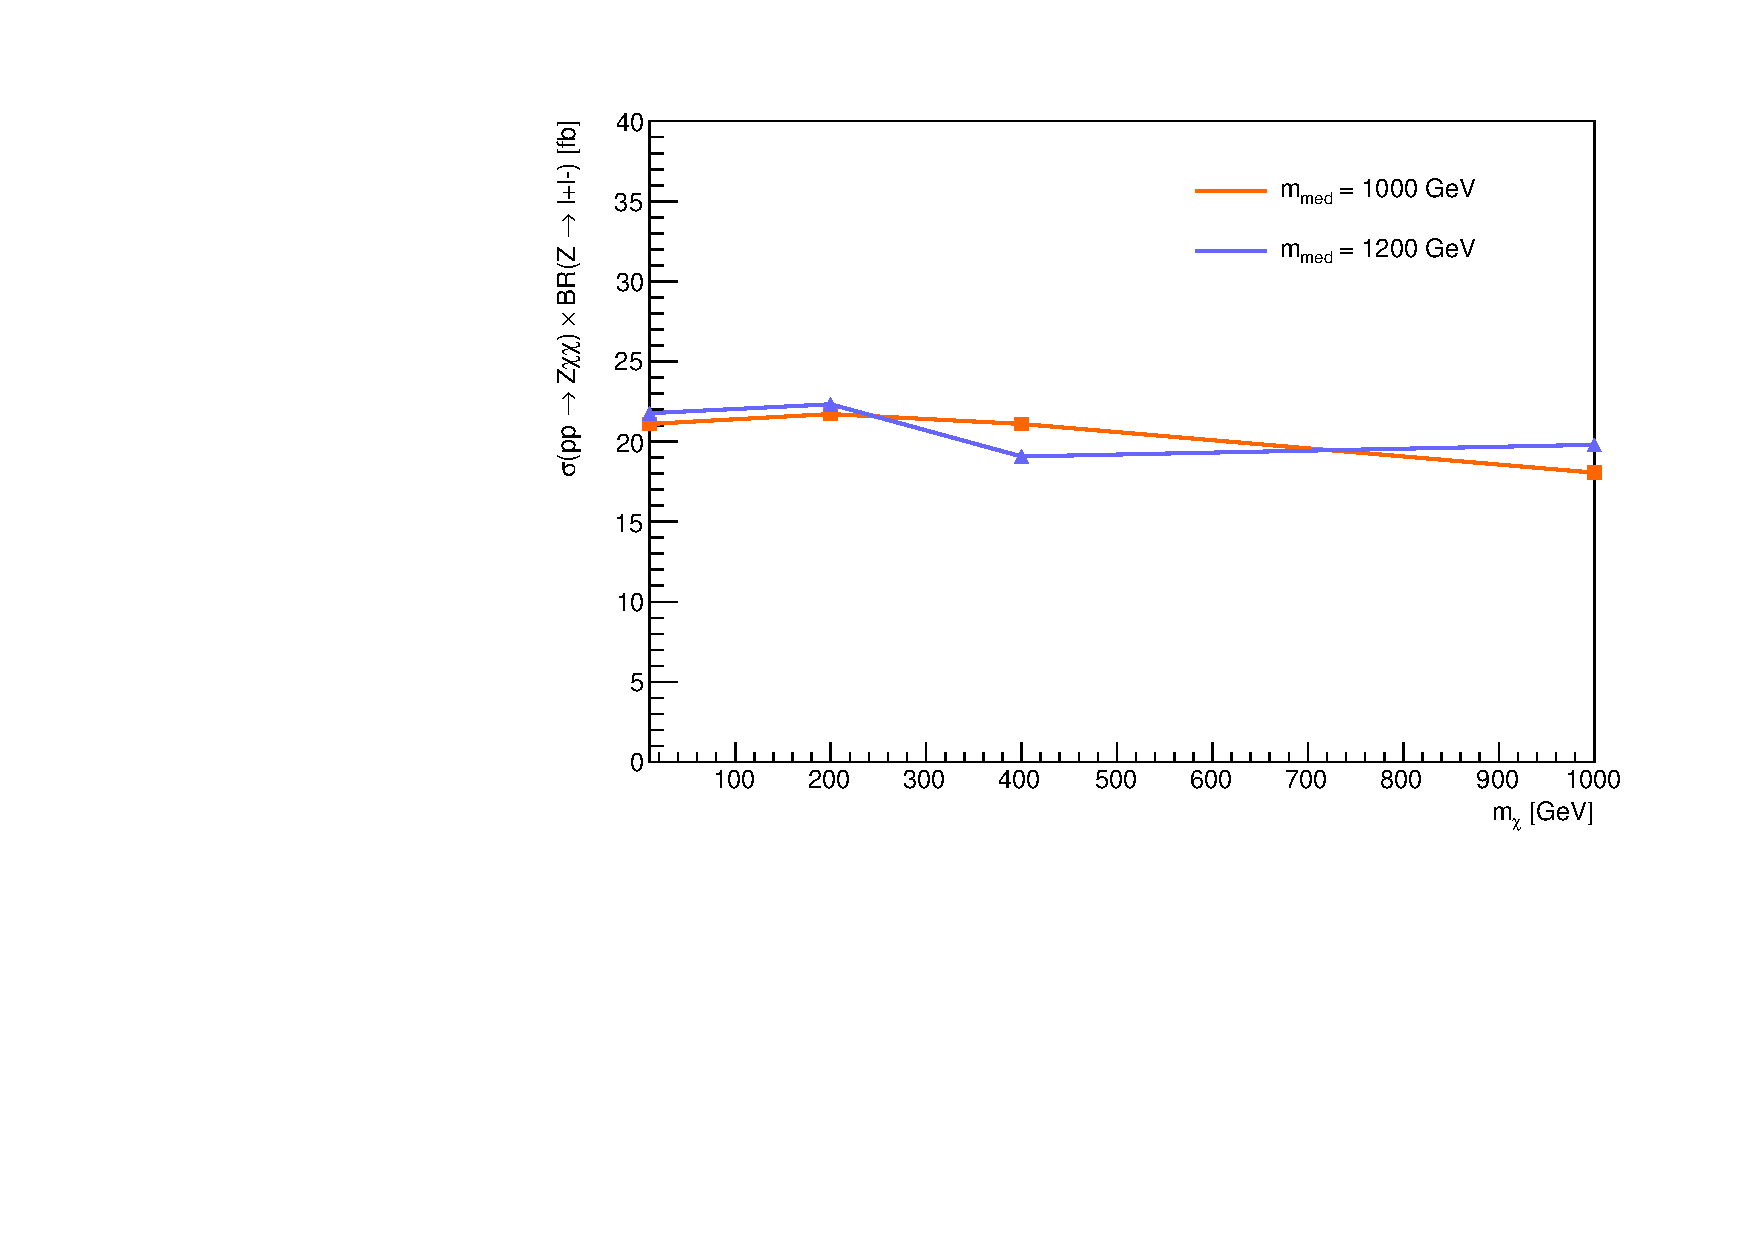
\includegraphics[width=0.45\textwidth]{figures/monoZ_sigma_limits_variedDMmass.pdf}
\caption{Mono-Z channel, tS model. REPLACE WITH TS MODEL PLOTS.}
\label{fig:MonoZ_TSD_limit}
\end{center} 
\end{figure}

\begin{figure}[!h]
\begin{center}
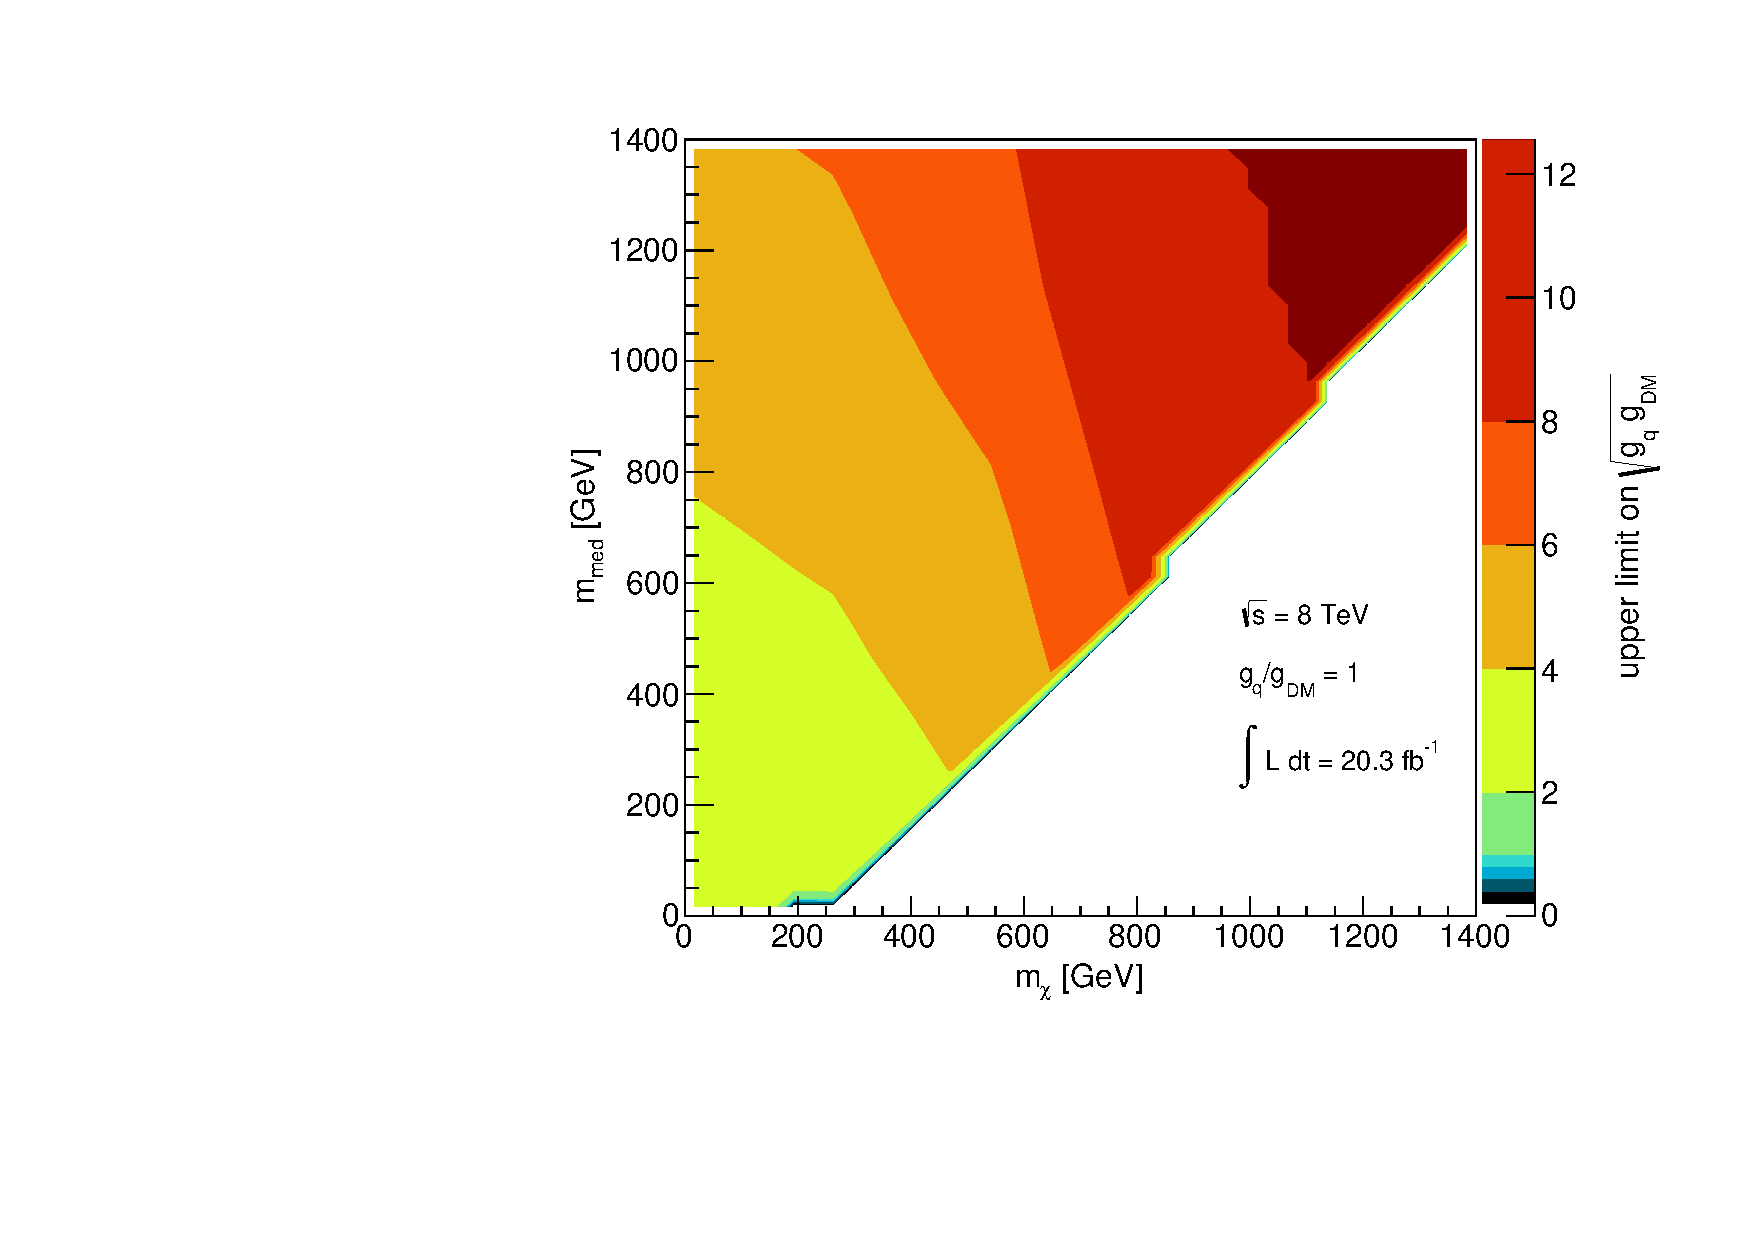
\includegraphics[width=0.45\textwidth]{figures/coupling_limits_TSD_1.pdf}
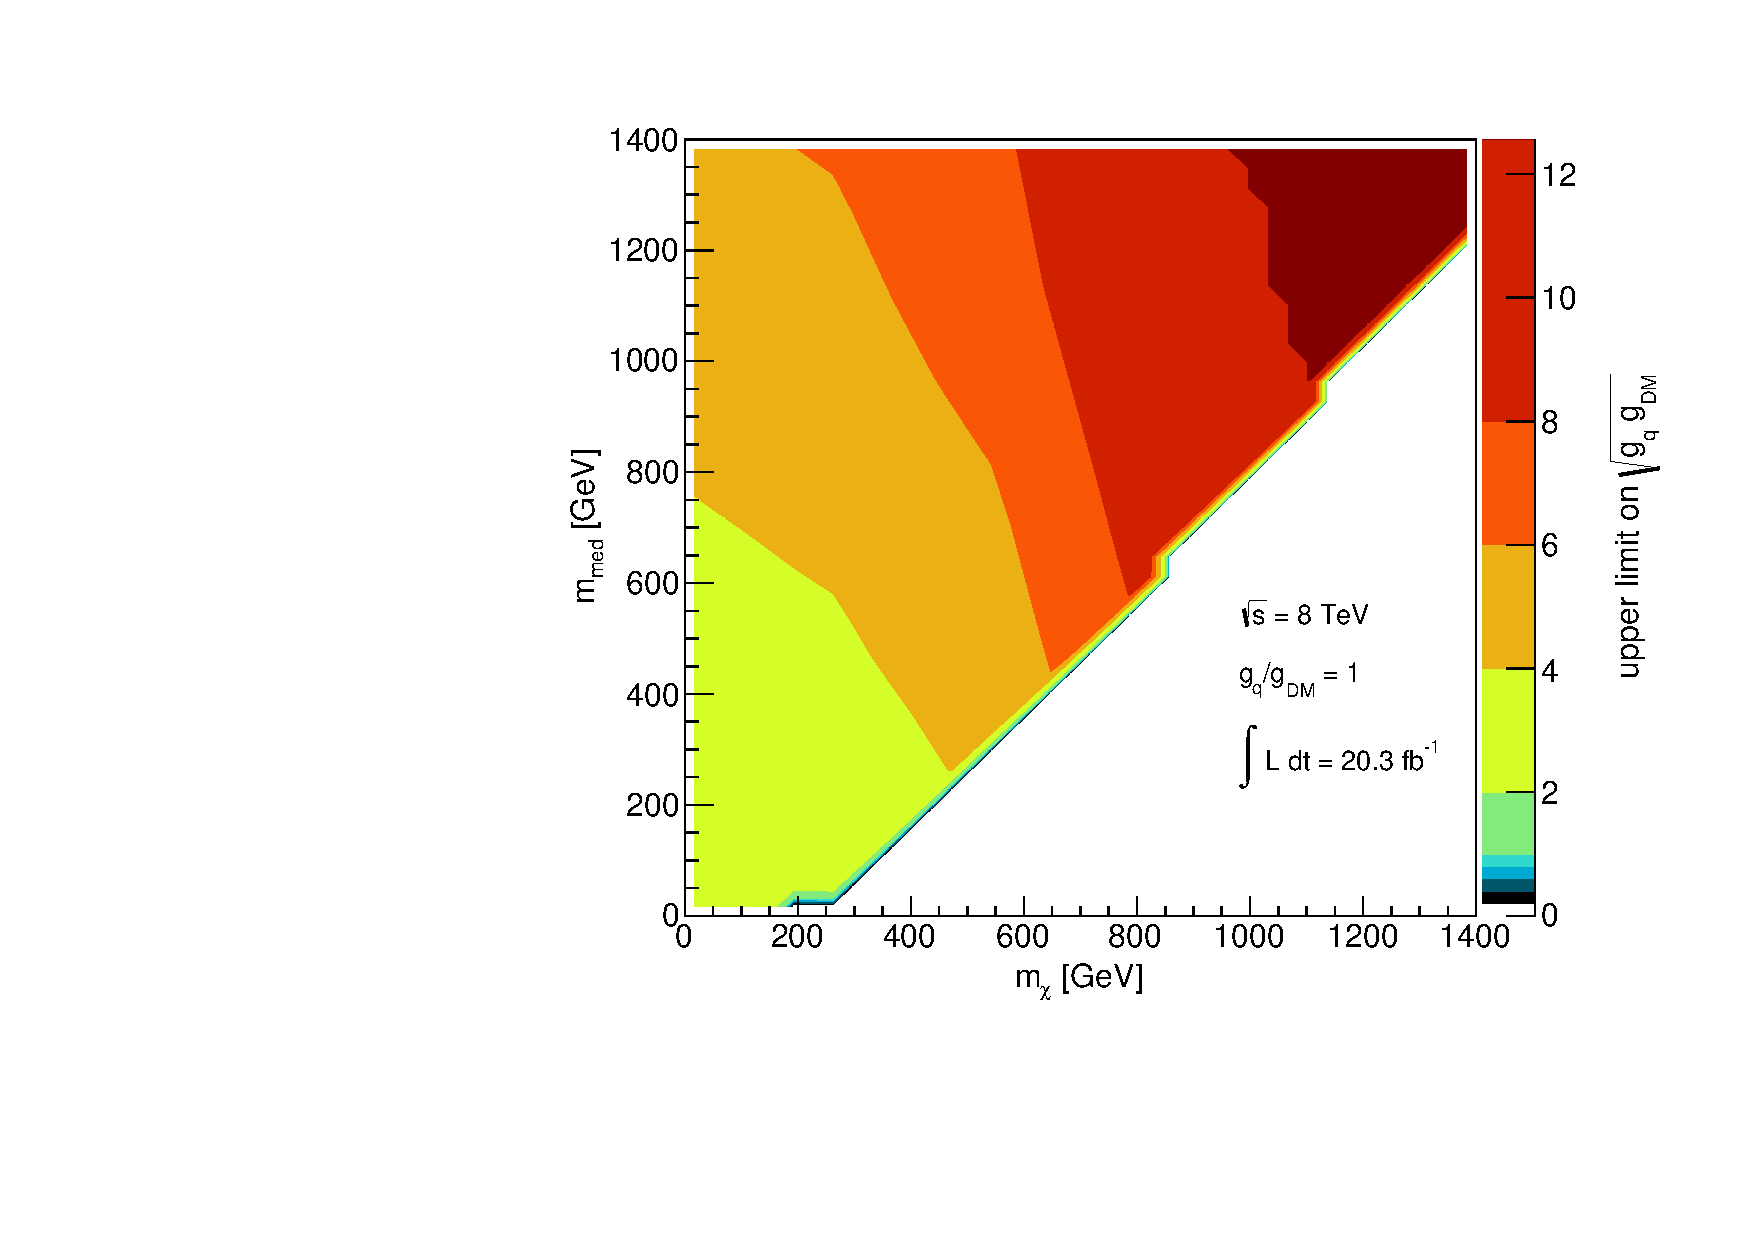
\includegraphics[width=0.45\textwidth]{figures/coupling_limits_TSD_1.pdf}
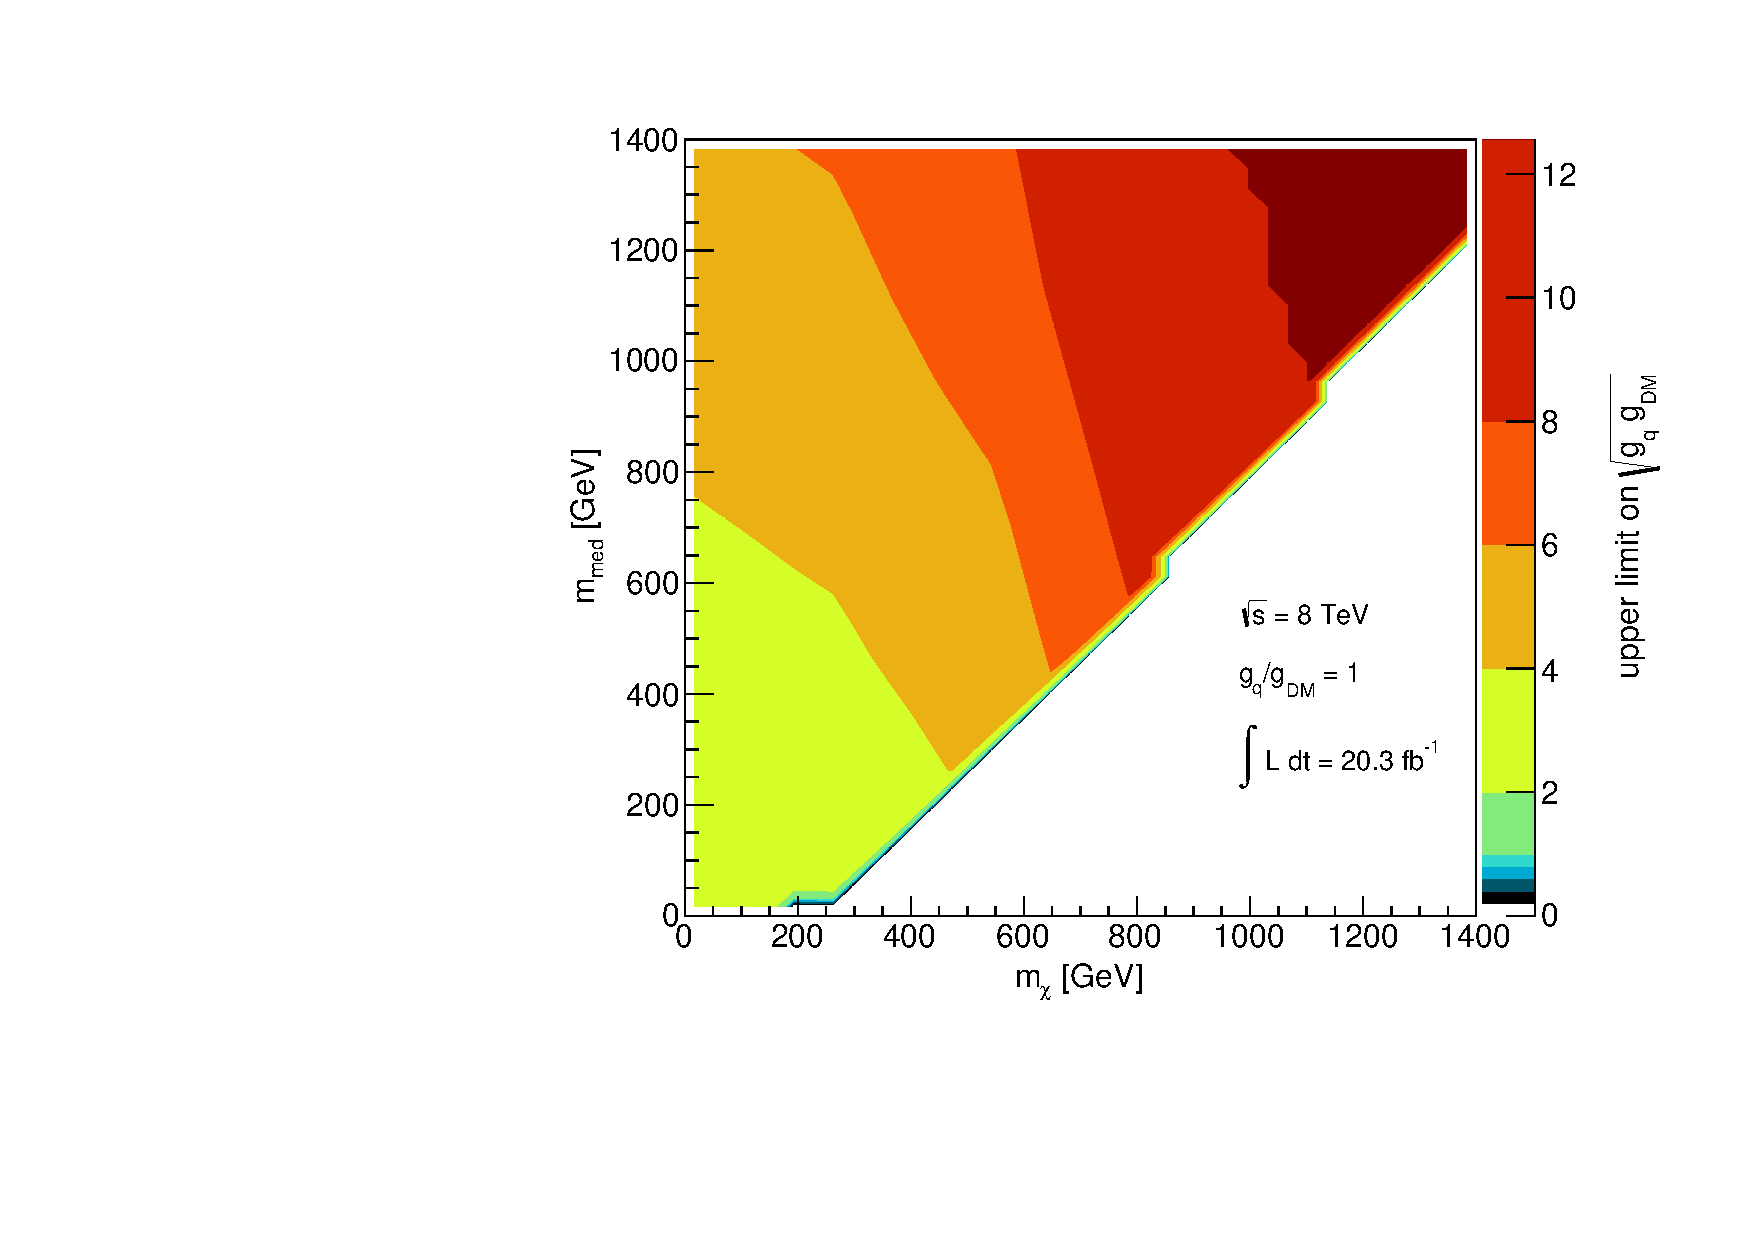
\includegraphics[width=0.45\textwidth]{figures/coupling_limits_TSD_1.pdf}
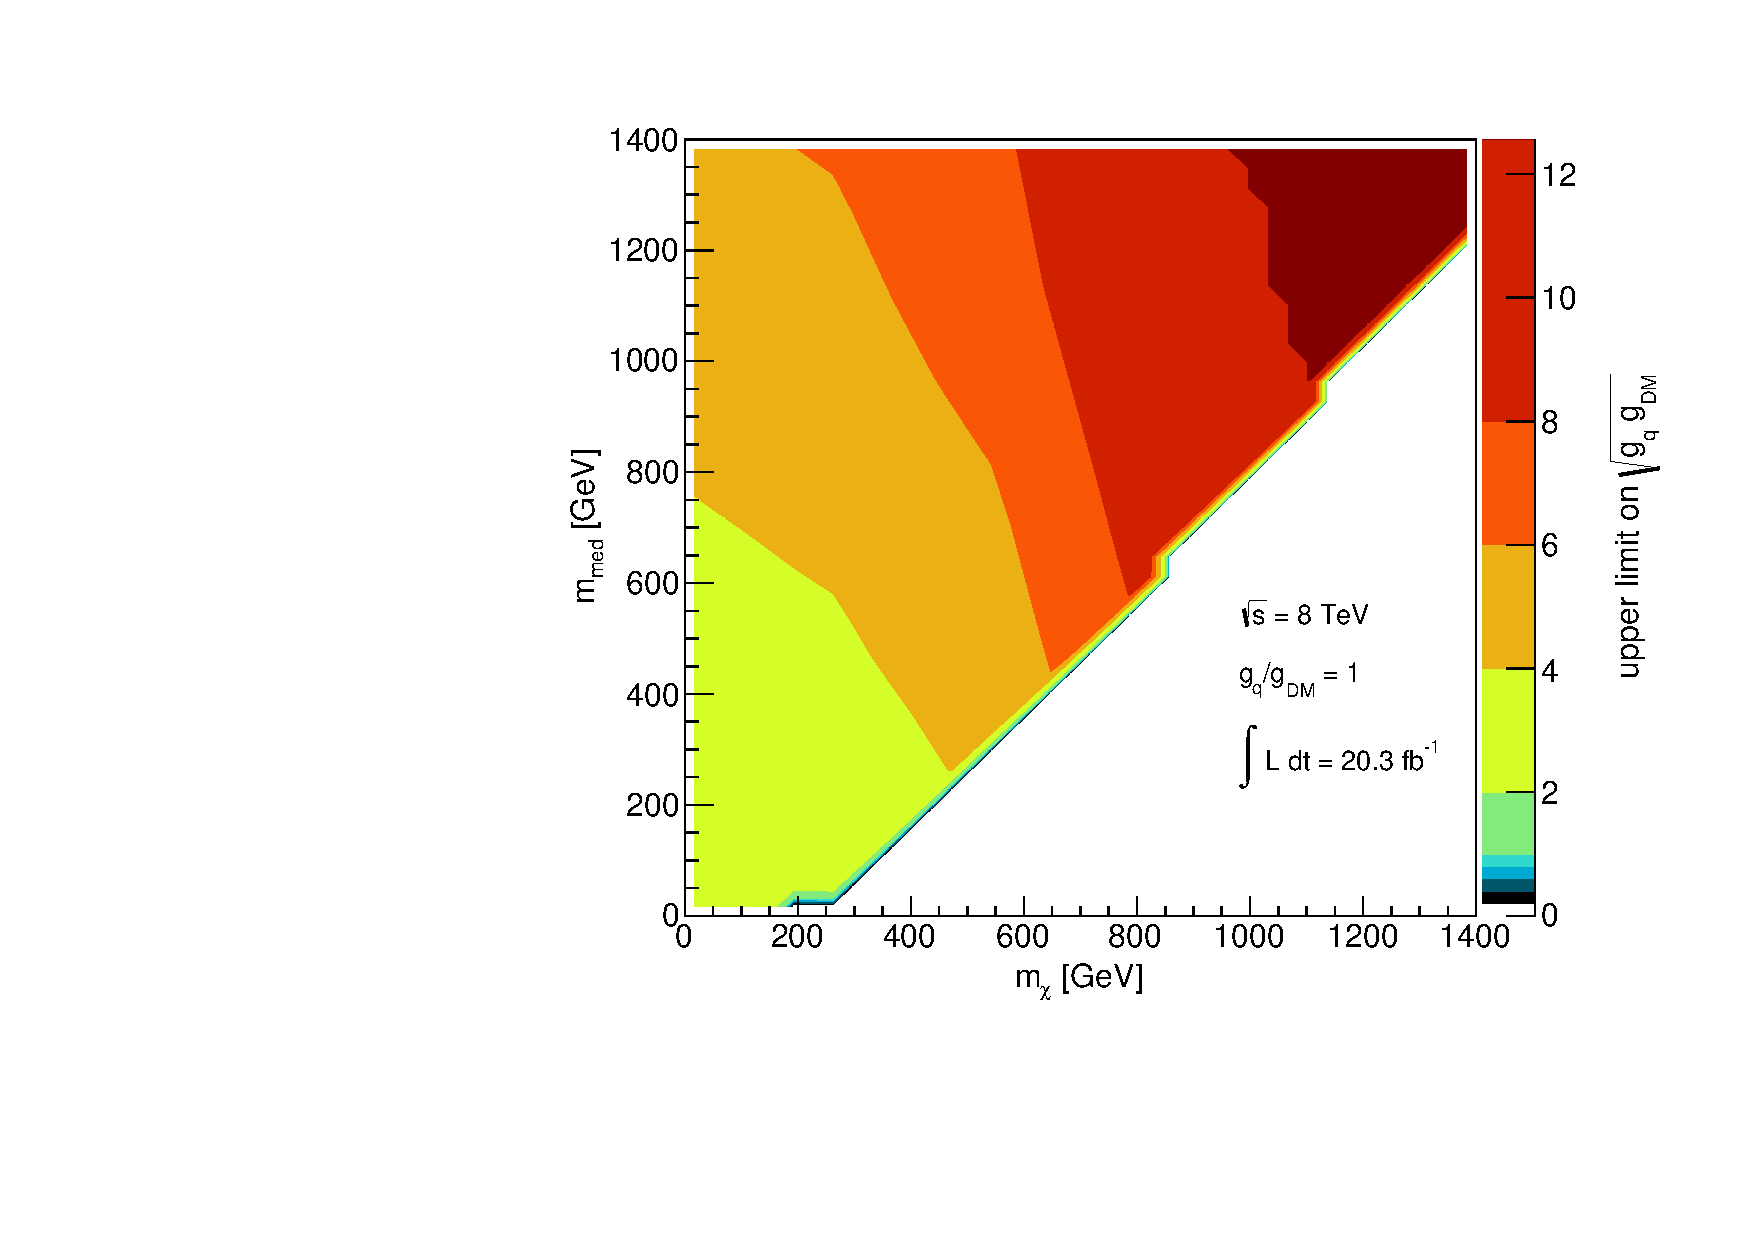
\includegraphics[width=0.45\textwidth]{figures/coupling_limits_TSD_1.pdf}
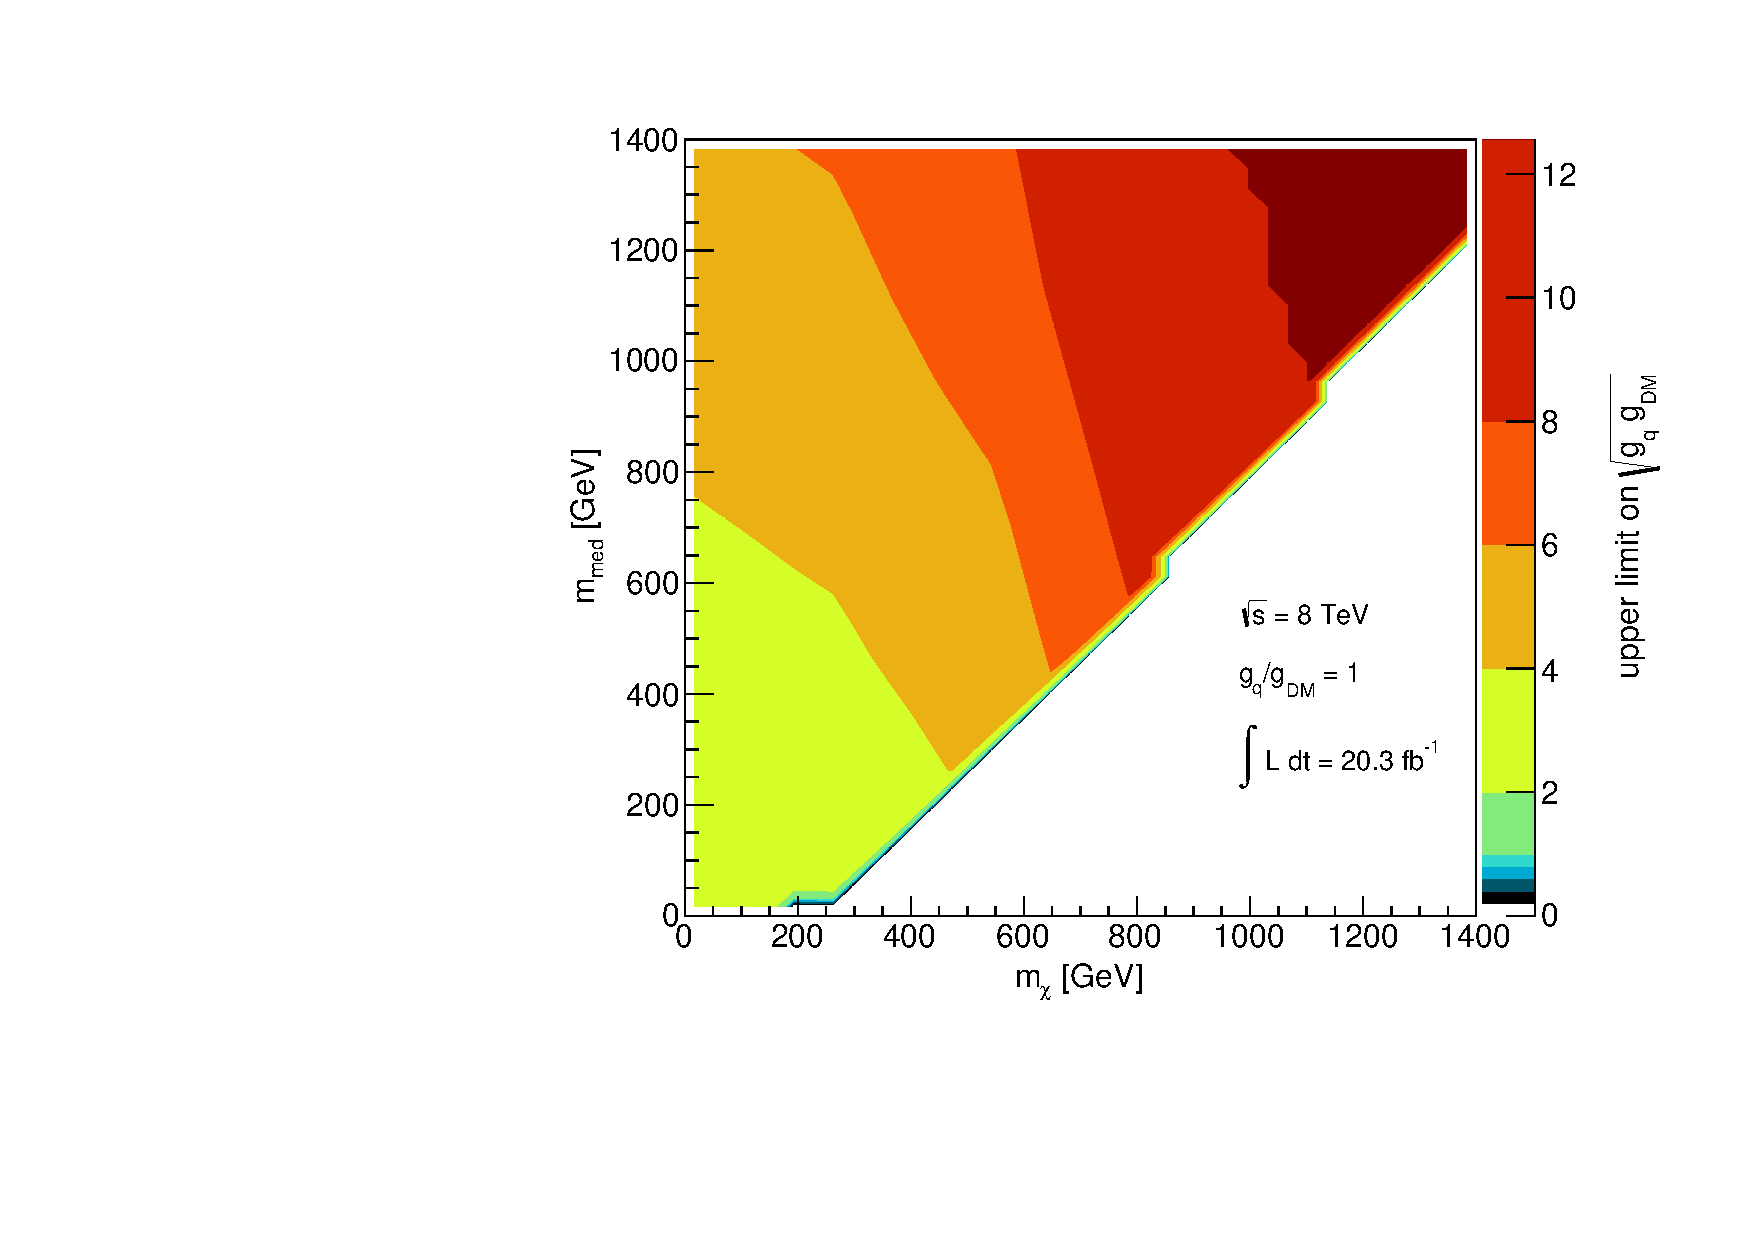
\includegraphics[width=0.45\textwidth]{figures/coupling_limits_TSD_1.pdf}
\caption{tS model coupling limit. REPLACE WITH TS MODEL PLOTS.}
\label{fig:MonoZ_TSD_couplinglimit}
\end{center}
\end{figure}

\subsection{Mono-$Z$ channel}

\begin{figure}[!h]
\begin{center}
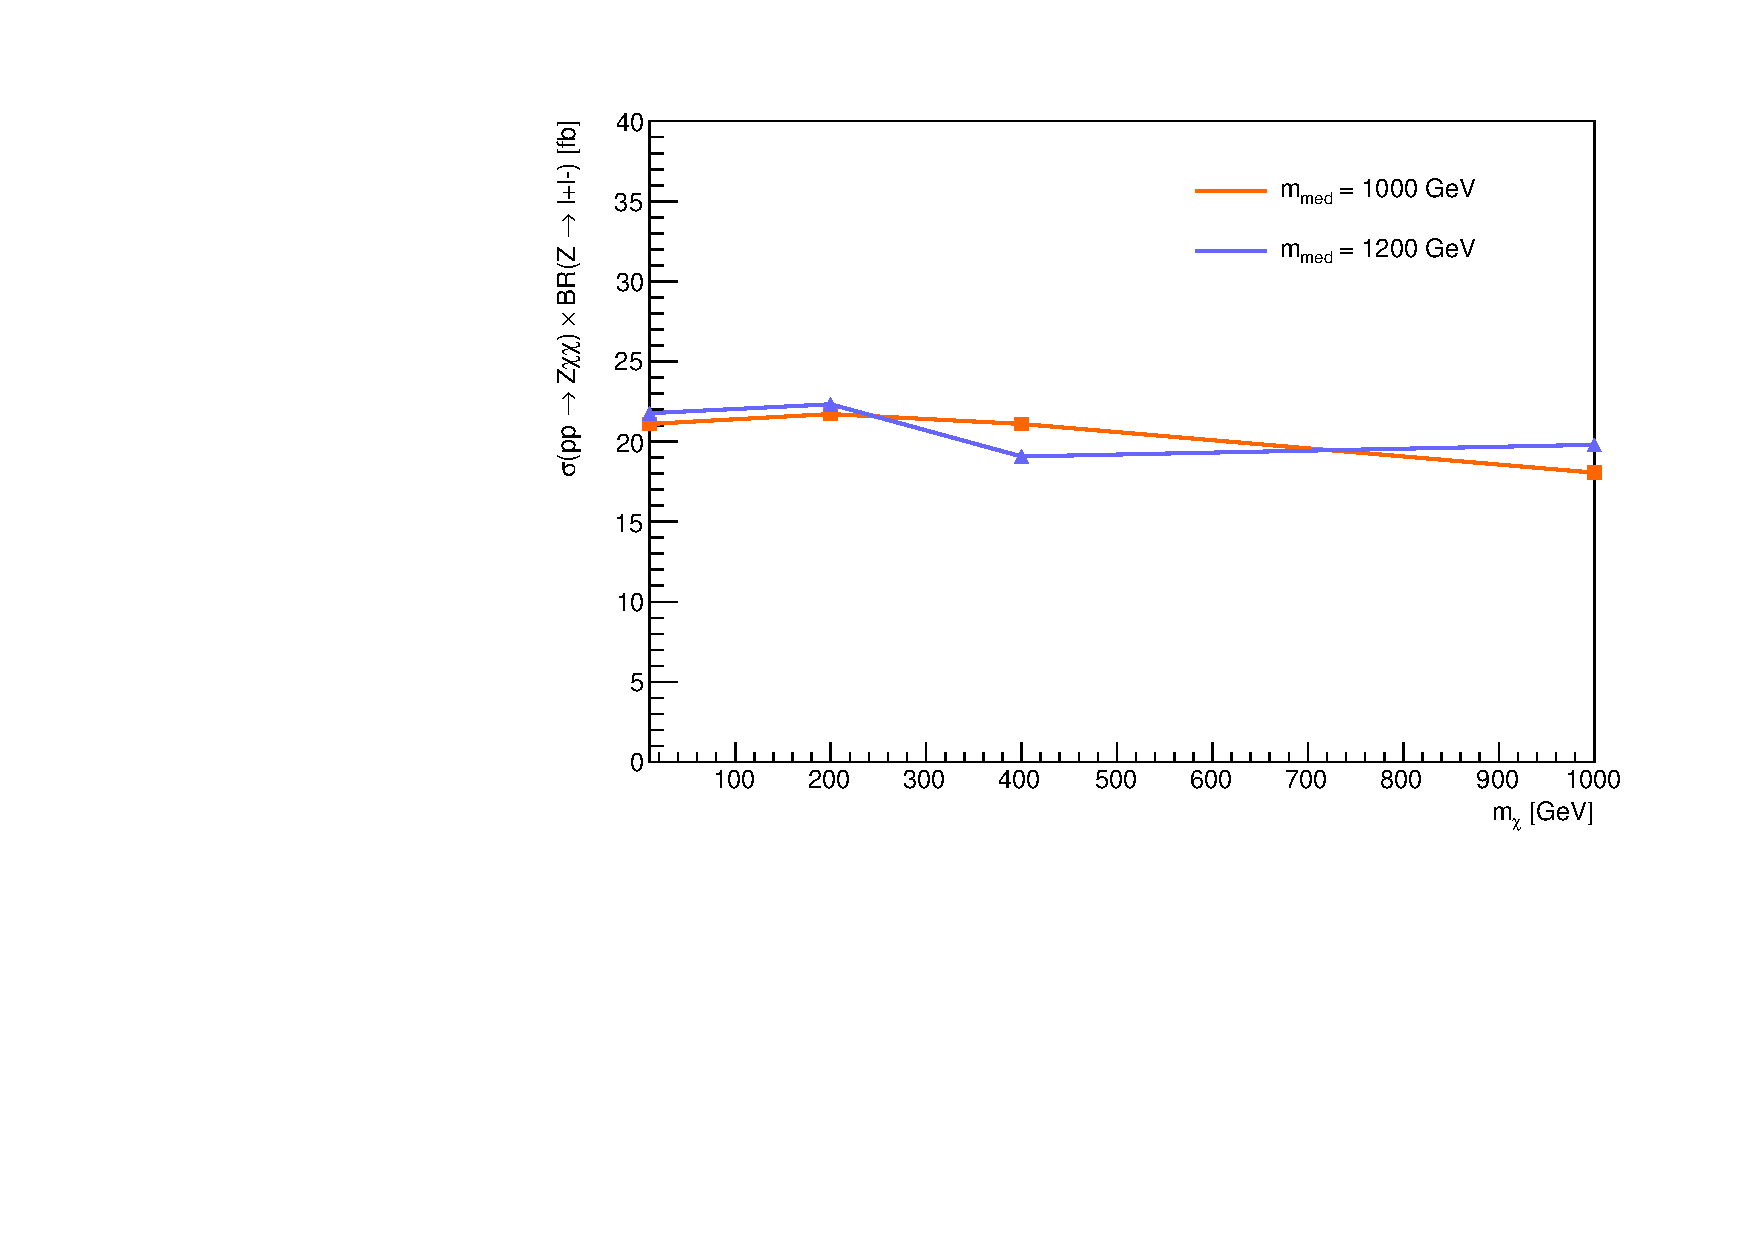
\includegraphics[width=0.45\textwidth]{figures/monoZ_sigma_limits_variedDMmass.pdf}
\caption{A very rough first plot - to be prettified! Shows the limit on sigma x BR for the sV model in the mono-Z channel. Will change to have a band for the expected limit, and a line for the observed limit. Show 5 different coupling scenarios on one plot. Mono-Z channel, sV model.}
\label{fig:MonoZ_SVD_limit}
\end{center}
\end{figure}

\begin{figure}[!h]
\begin{center}
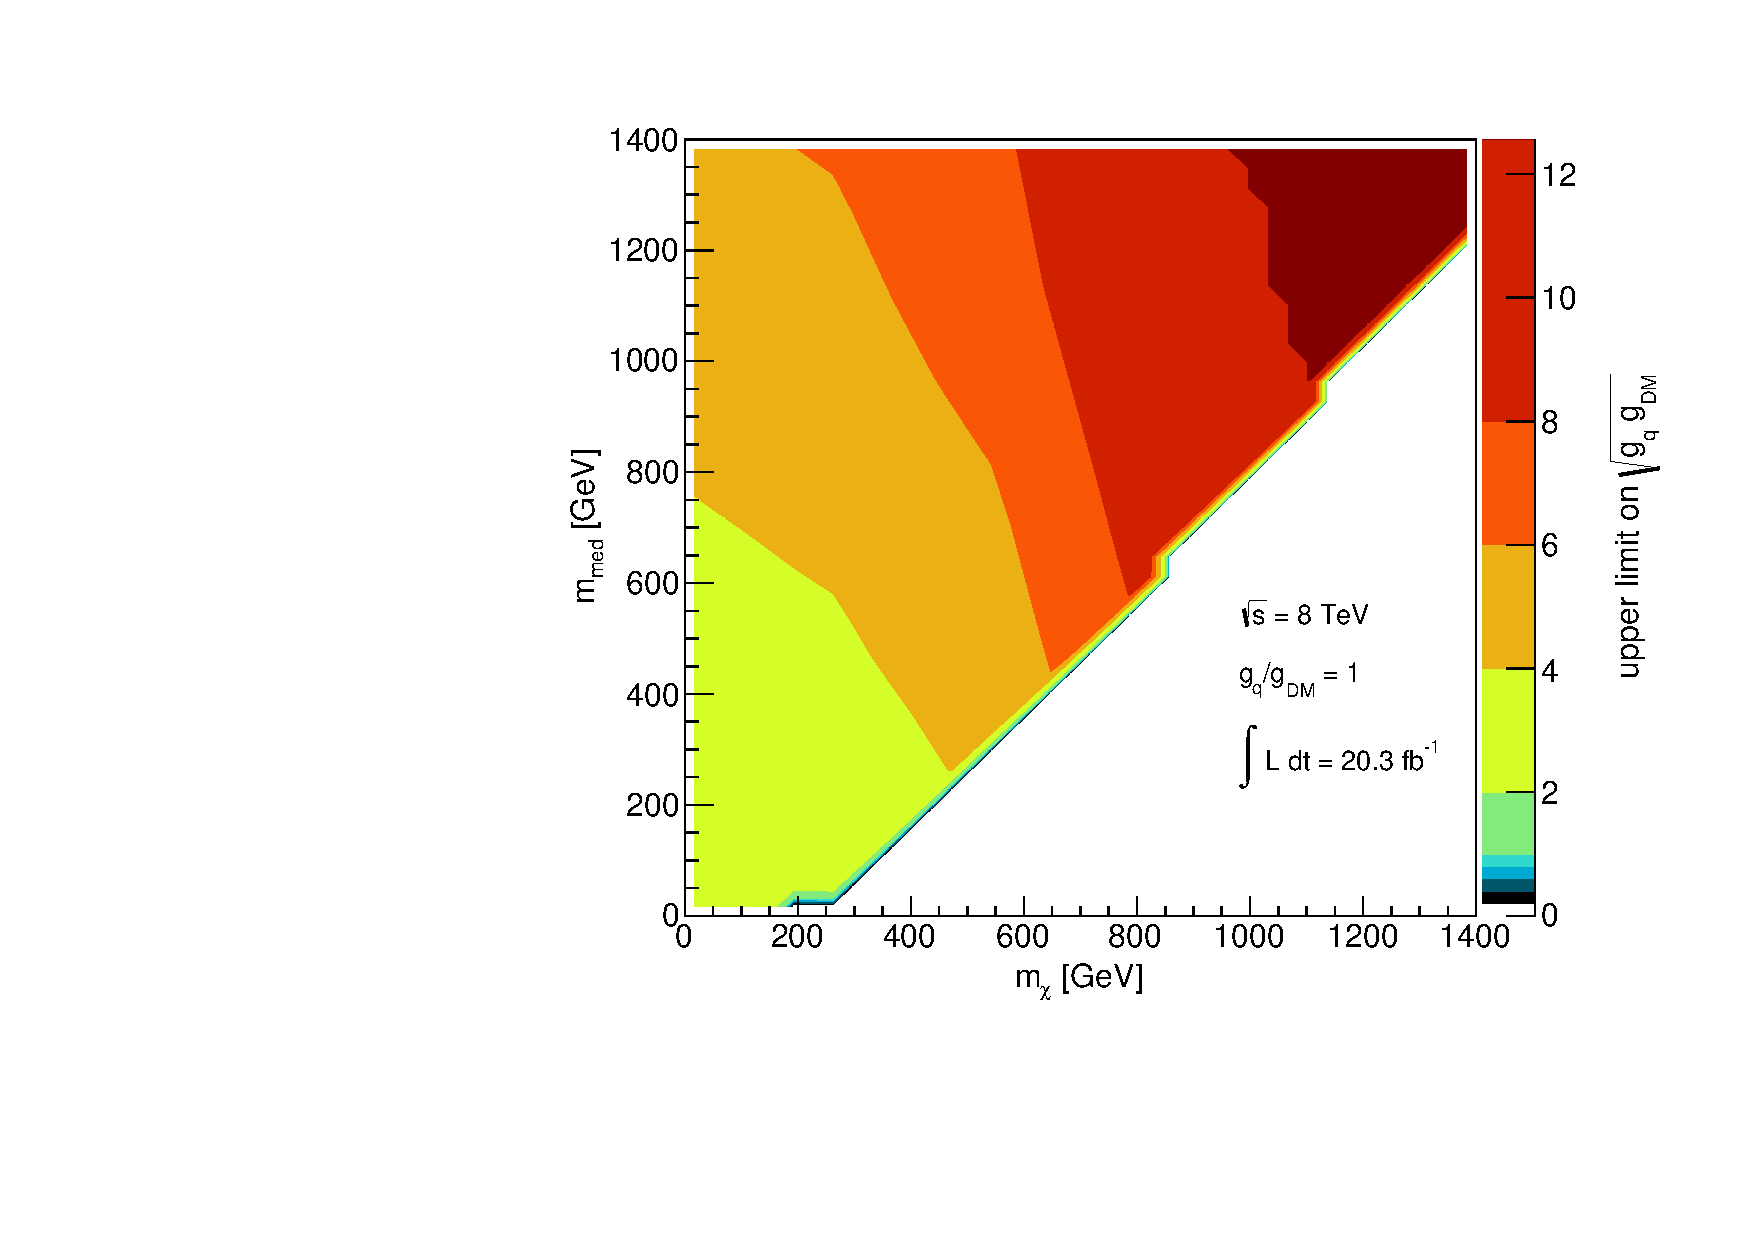
\includegraphics[width=0.45\textwidth]{figures/coupling_limits_TSD_1.pdf}
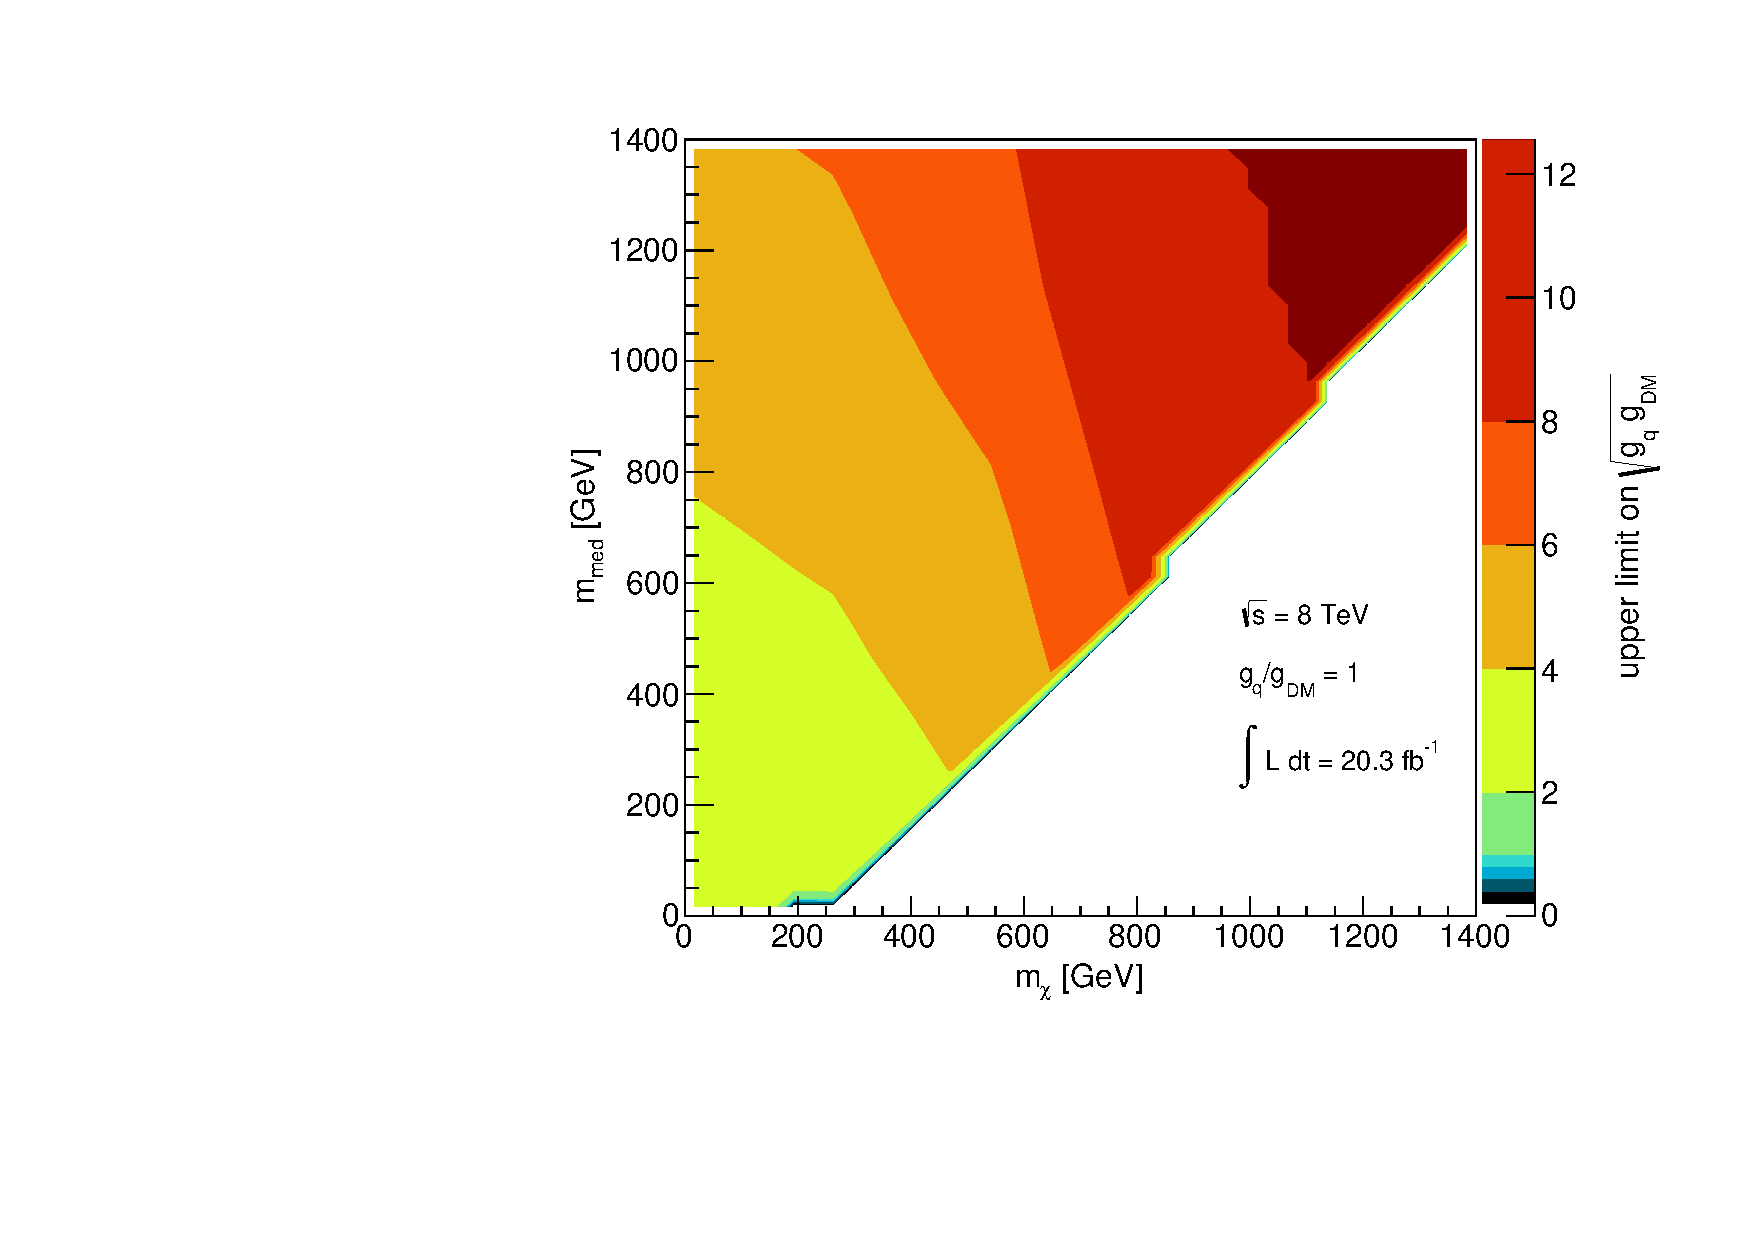
\includegraphics[width=0.45\textwidth]{figures/coupling_limits_TSD_1.pdf}
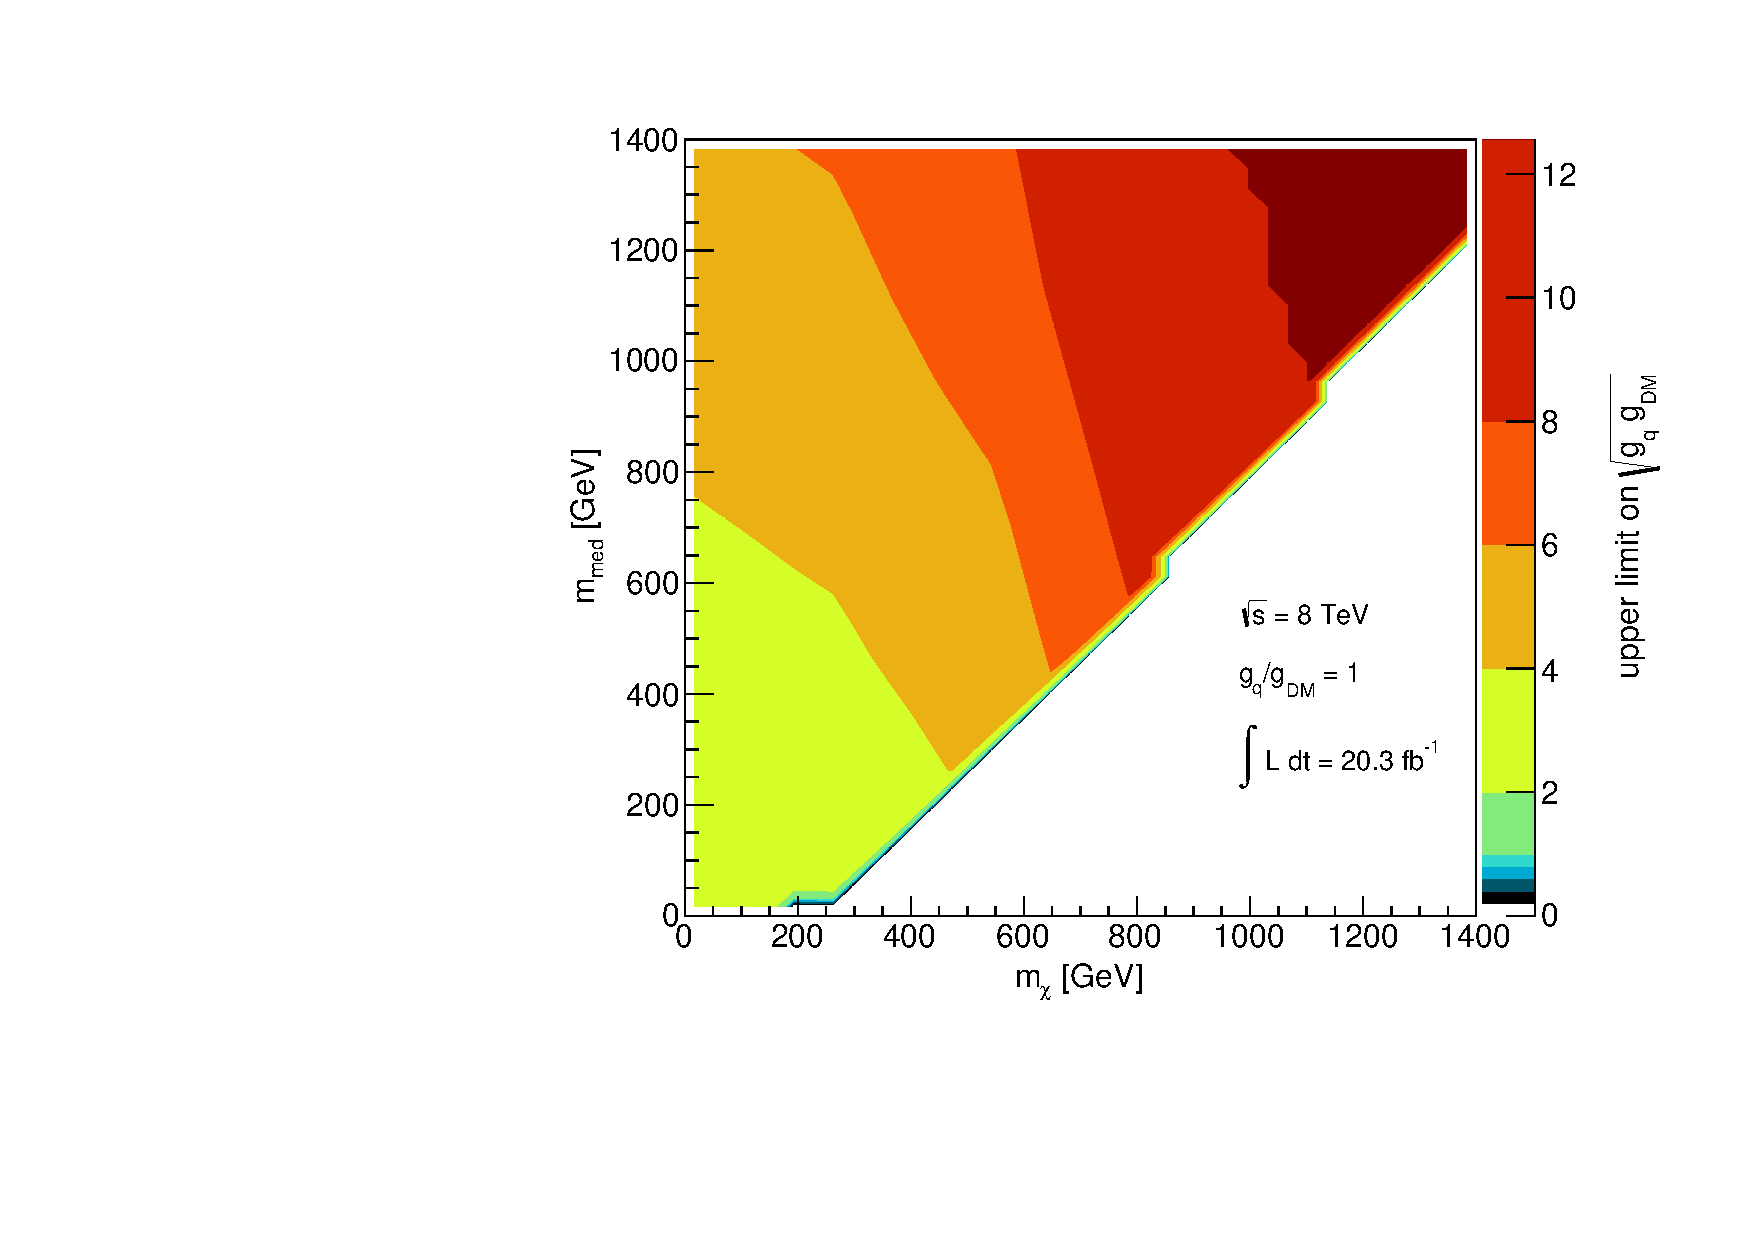
\includegraphics[width=0.45\textwidth]{figures/coupling_limits_TSD_1.pdf}
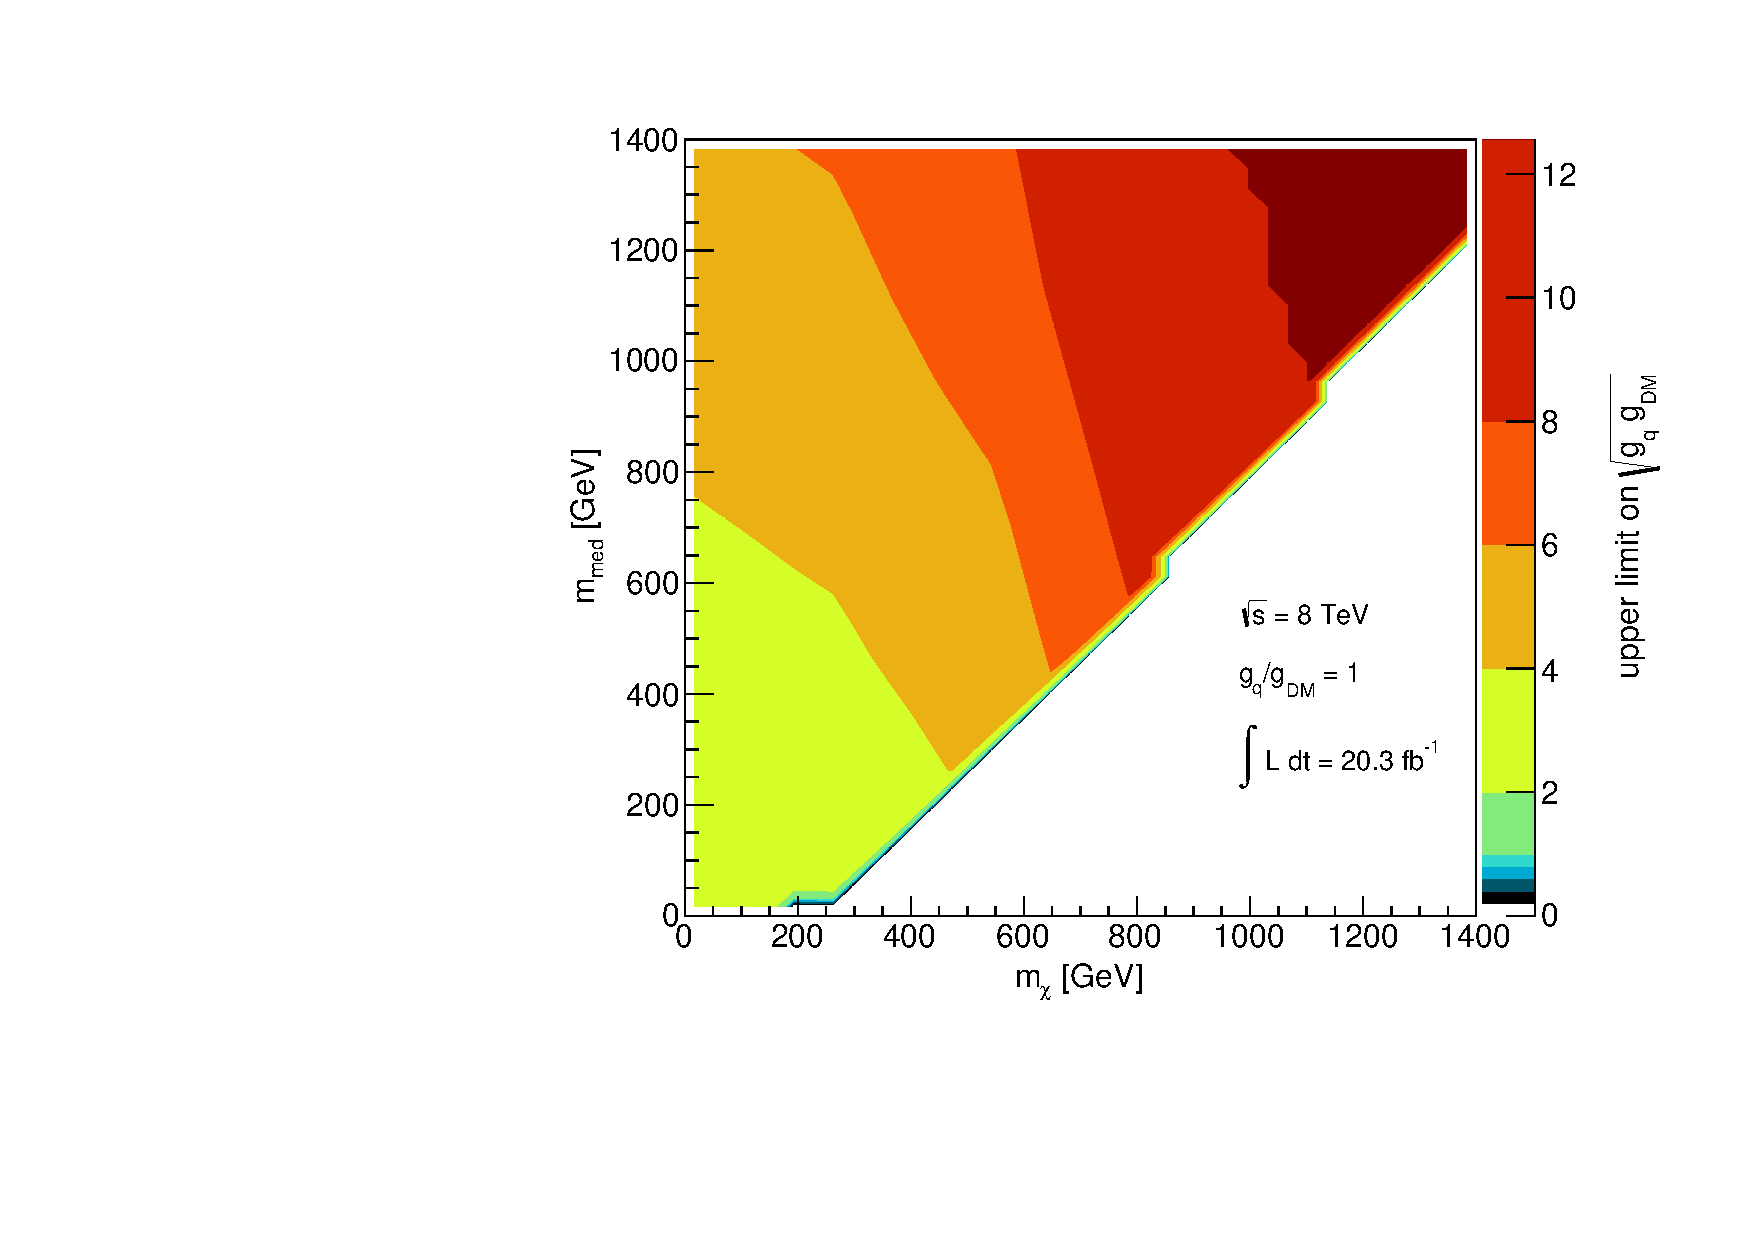
\includegraphics[width=0.45\textwidth]{figures/coupling_limits_TSD_1.pdf}
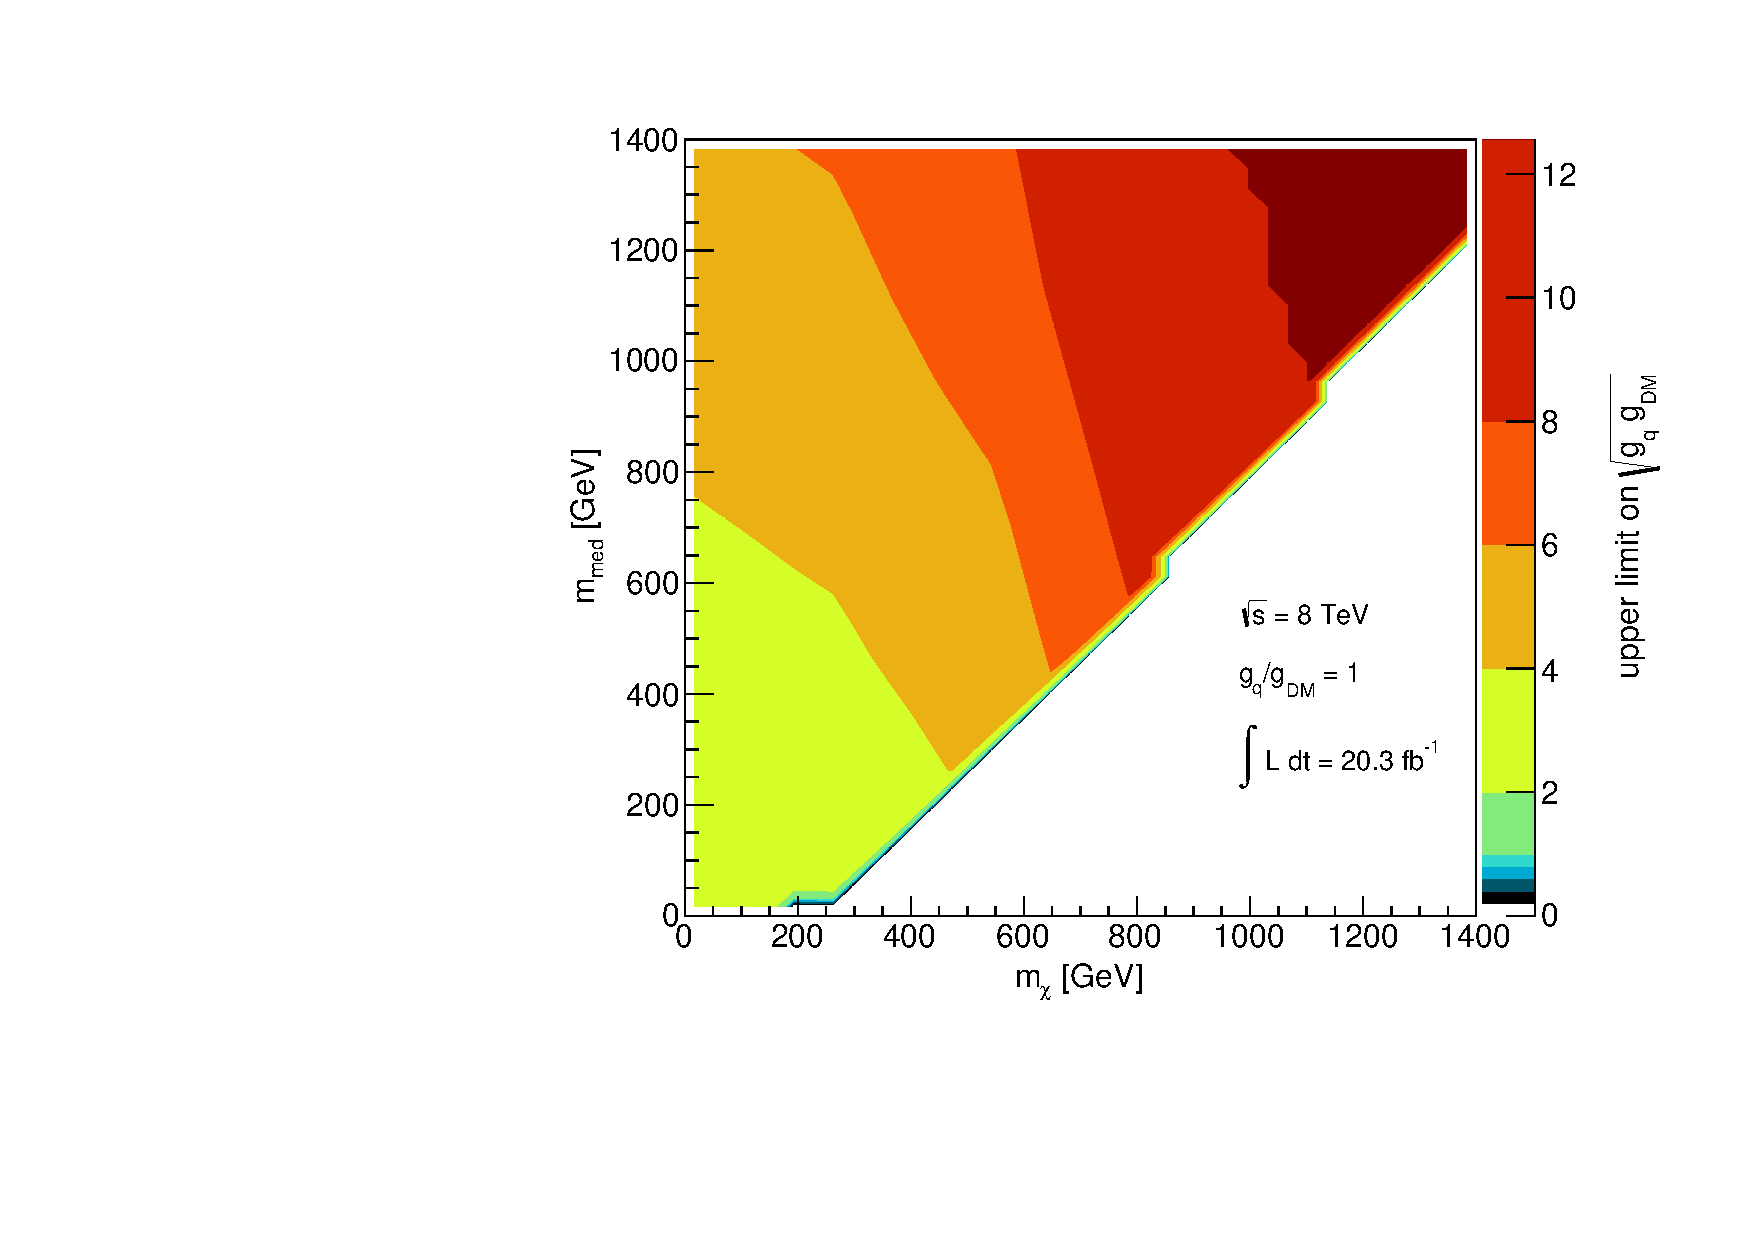
\includegraphics[width=0.45\textwidth]{figures/coupling_limits_TSD_1.pdf}
\caption{Limit on coupling strength for the sV model, in the mono-Z channel.  Need to fix up the scale on the z-axis and include mass points as dots on the plot. To be replaced with 5 plots with different coupling ratios, gq/gchi = 0.2, 0.5, 1, 2, 5. REPLACE WITH SV MODEL PLOTS.}
\label{fig:MonoZ_SVD_couplinglimit}
\end{center}
\end{figure}

\begin{figure}[!h]
\begin{center}
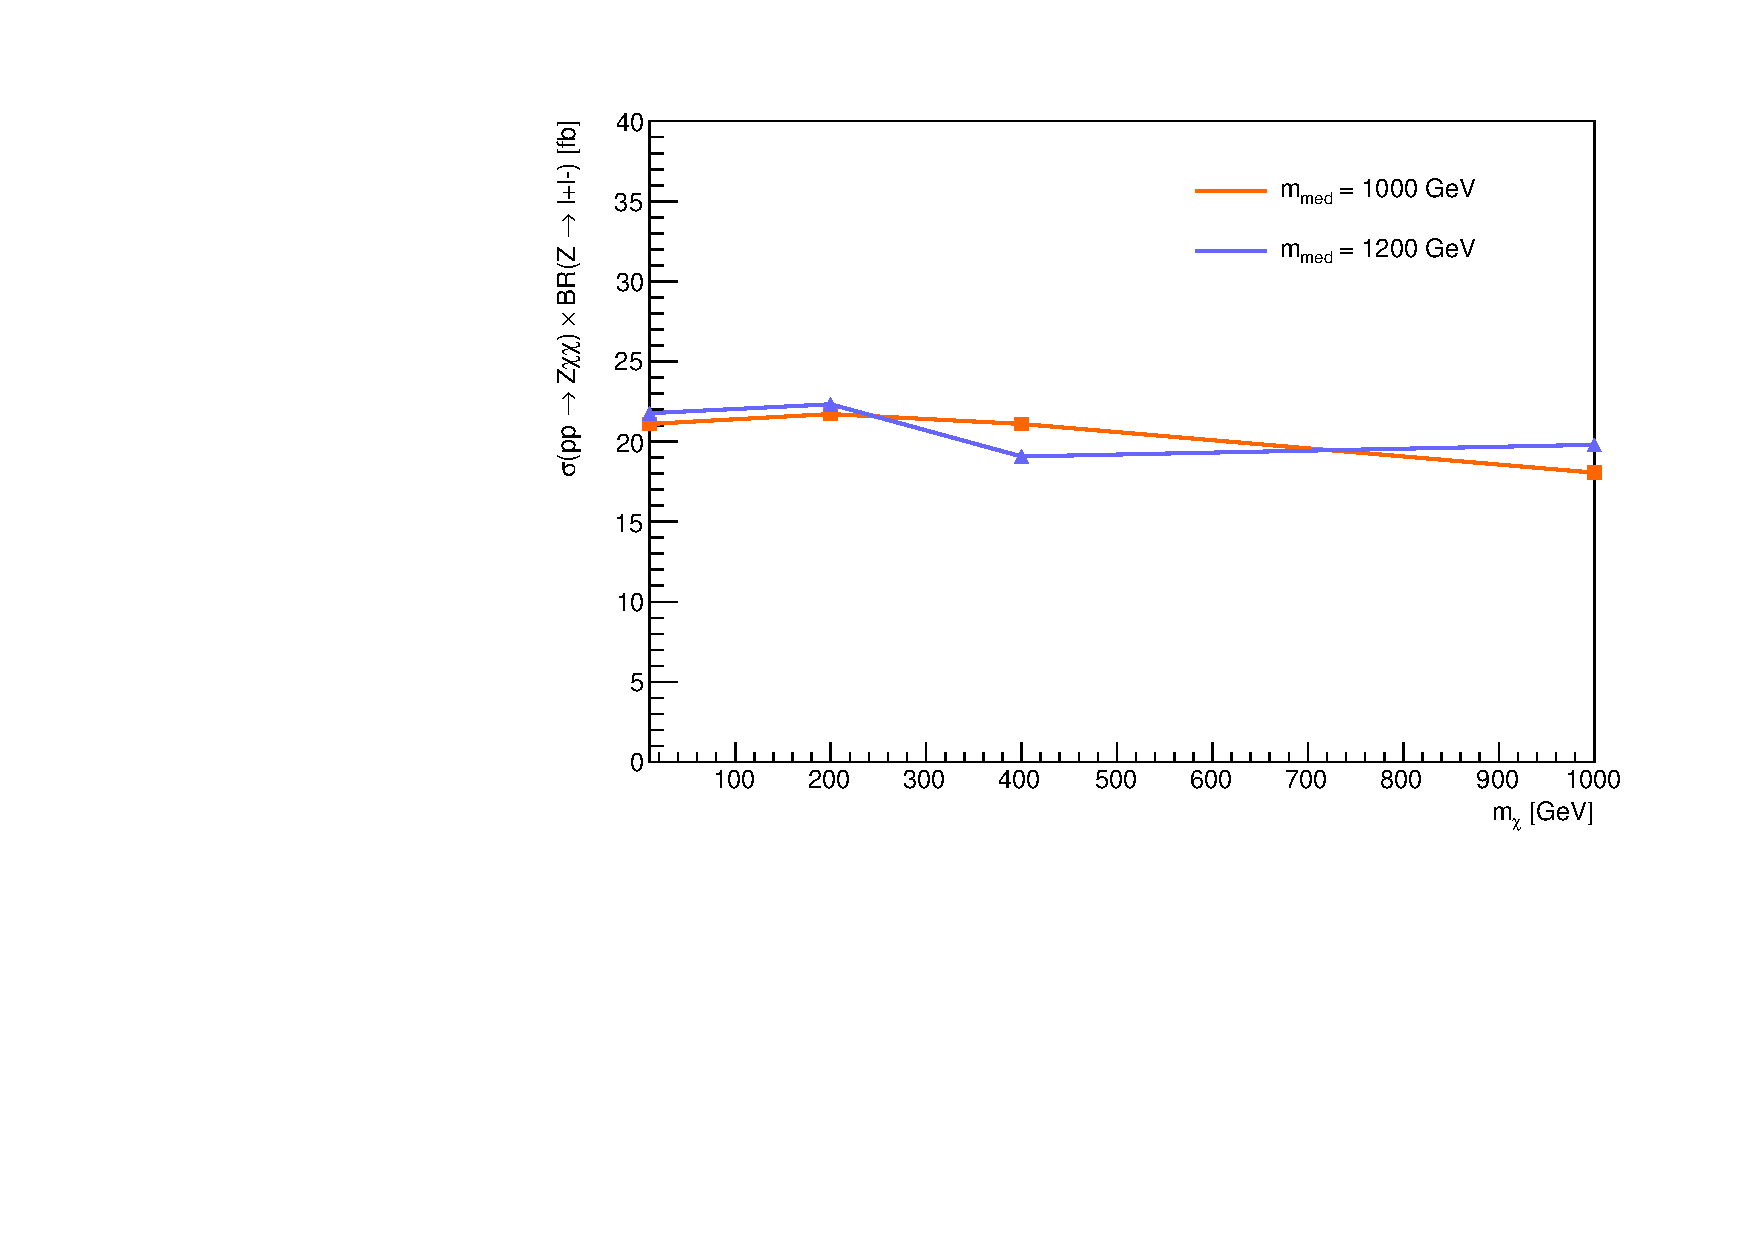
\includegraphics[width=0.45\textwidth]{figures/monoZ_sigma_limits_variedDMmass.pdf}
\caption{Mono-Z channel, sS model. REPLACE WITH SS MODEL PLOTS.}
\label{fig:MonoZ_SSD_limit}
\end{center}
\end{figure}

\begin{figure}[!h]
\begin{center}
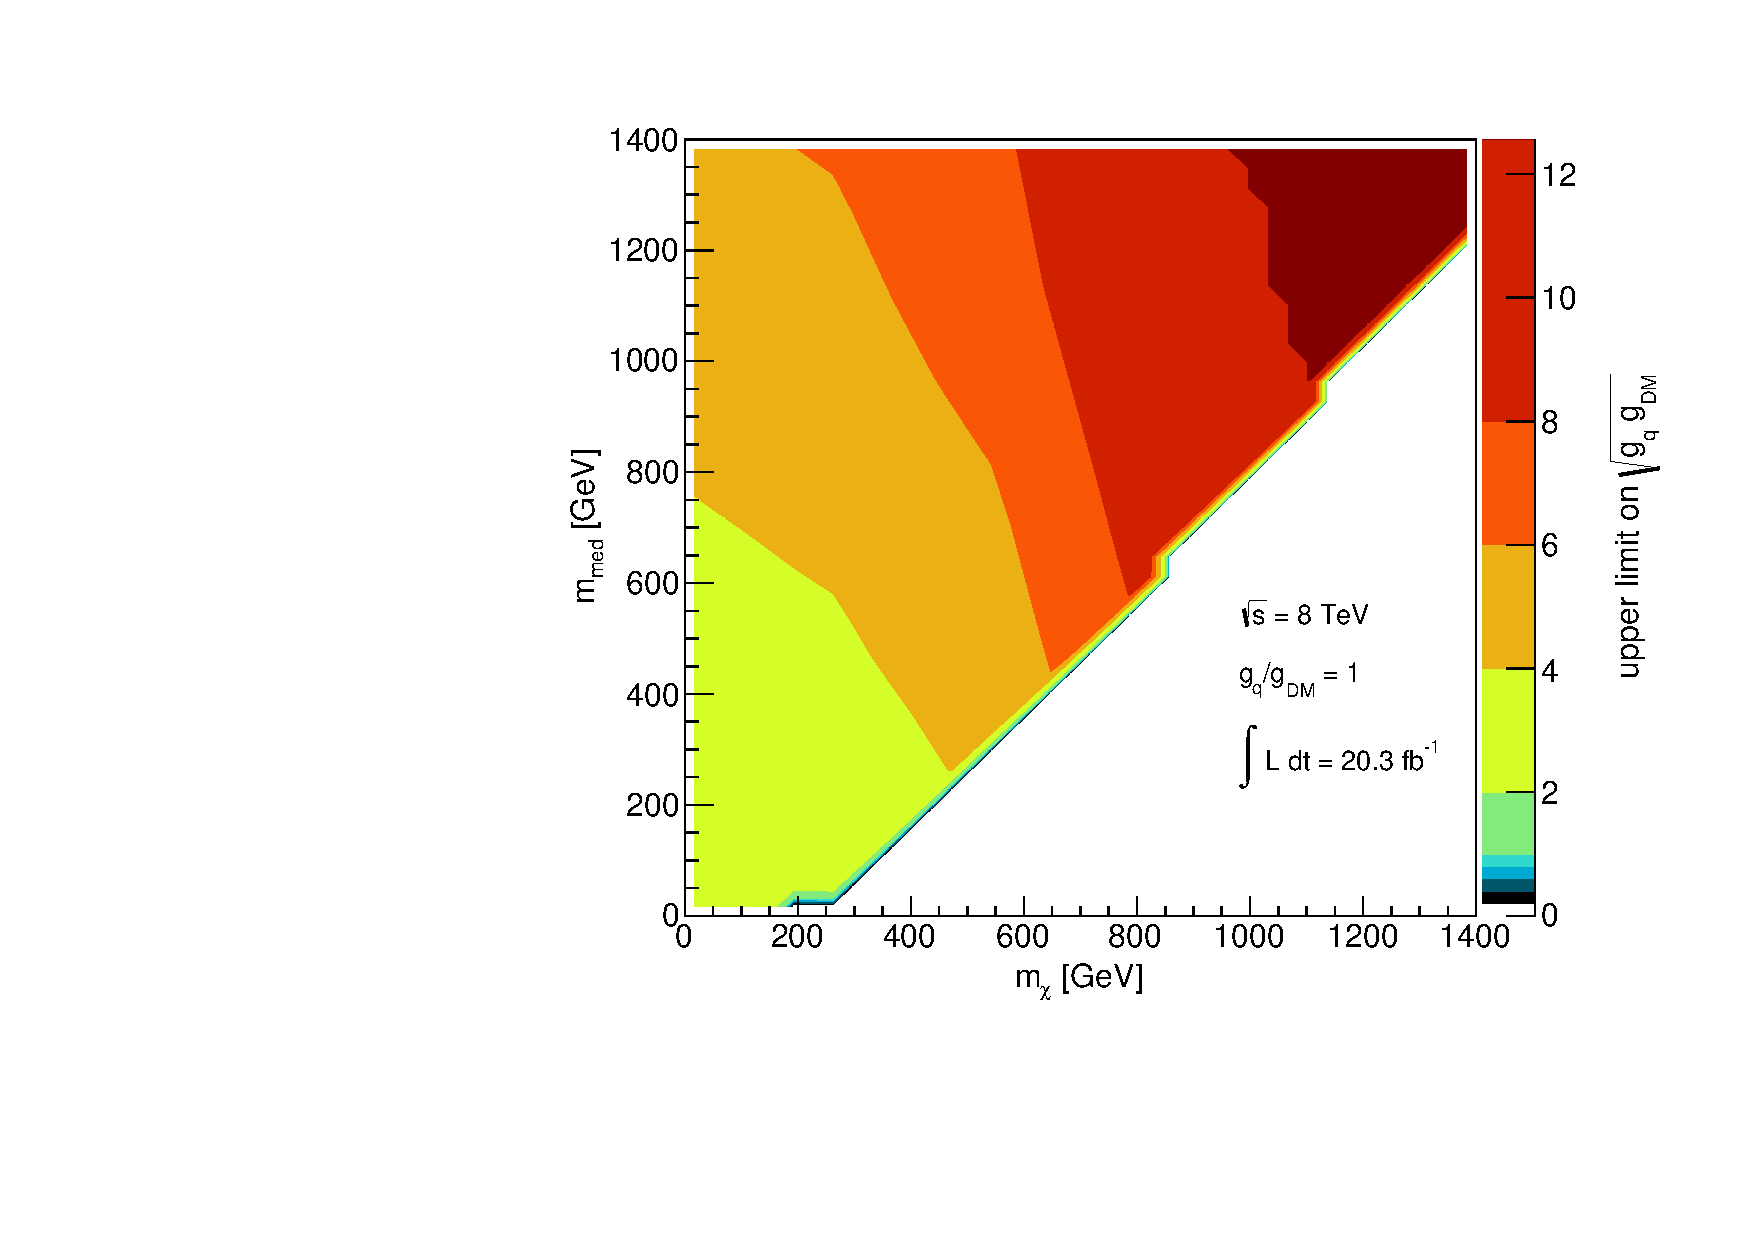
\includegraphics[width=0.45\textwidth]{figures/coupling_limits_TSD_1.pdf}
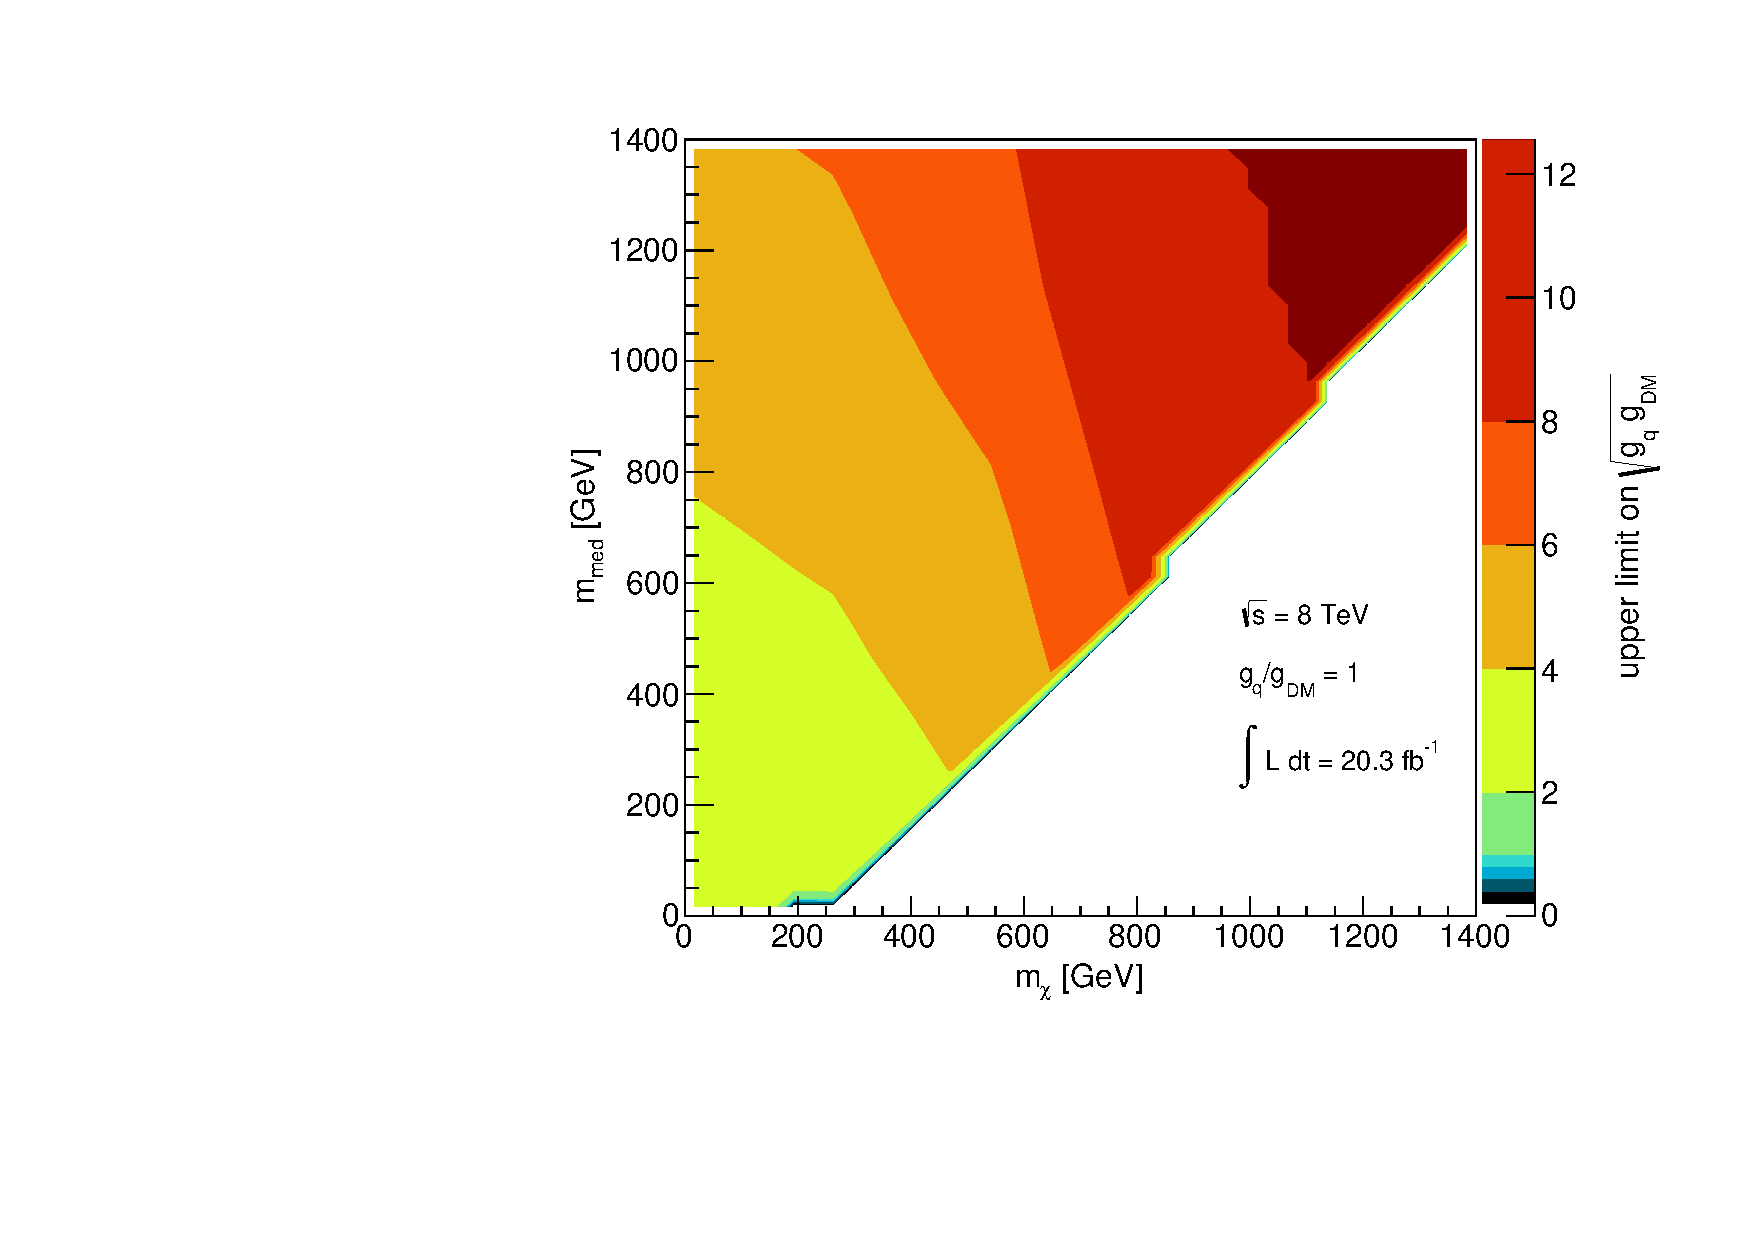
\includegraphics[width=0.45\textwidth]{figures/coupling_limits_TSD_1.pdf}
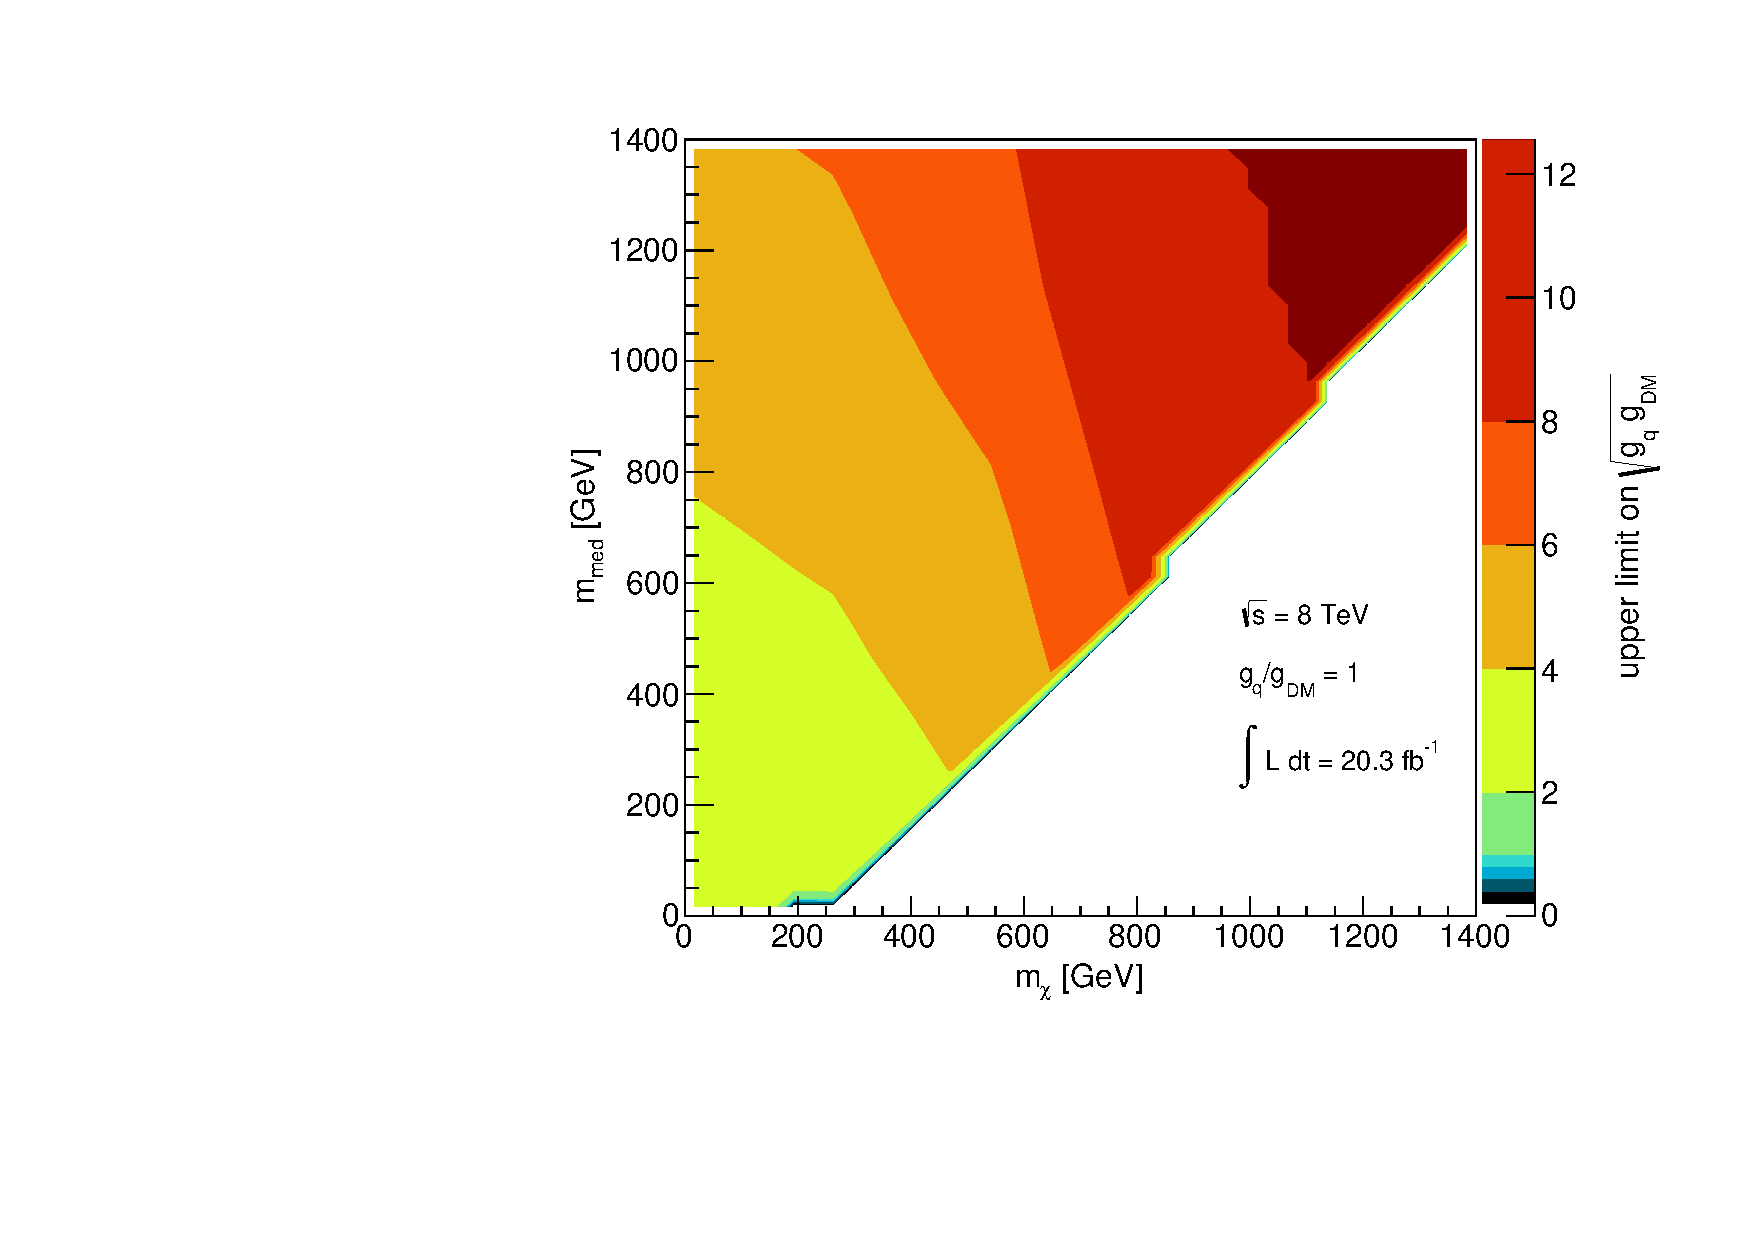
\includegraphics[width=0.45\textwidth]{figures/coupling_limits_TSD_1.pdf}
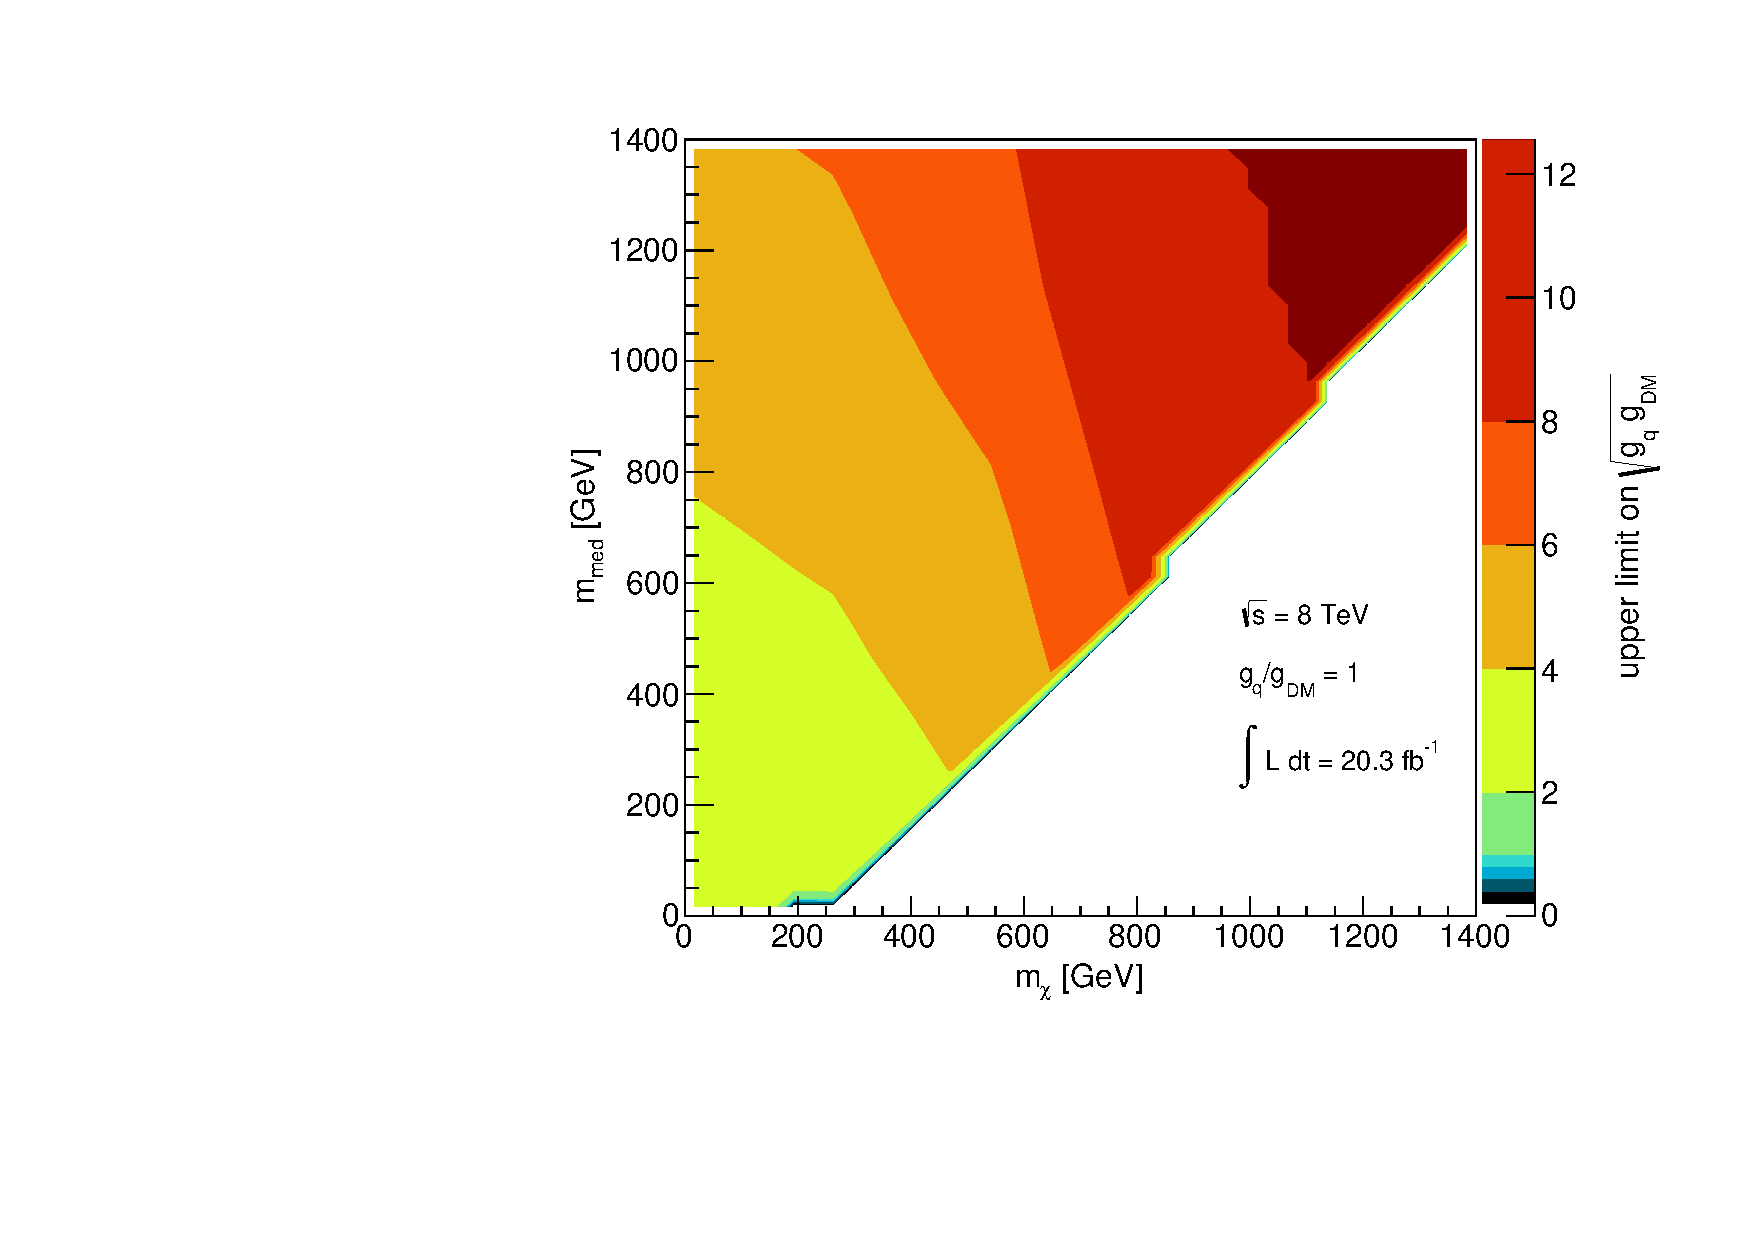
\includegraphics[width=0.45\textwidth]{figures/coupling_limits_TSD_1.pdf}
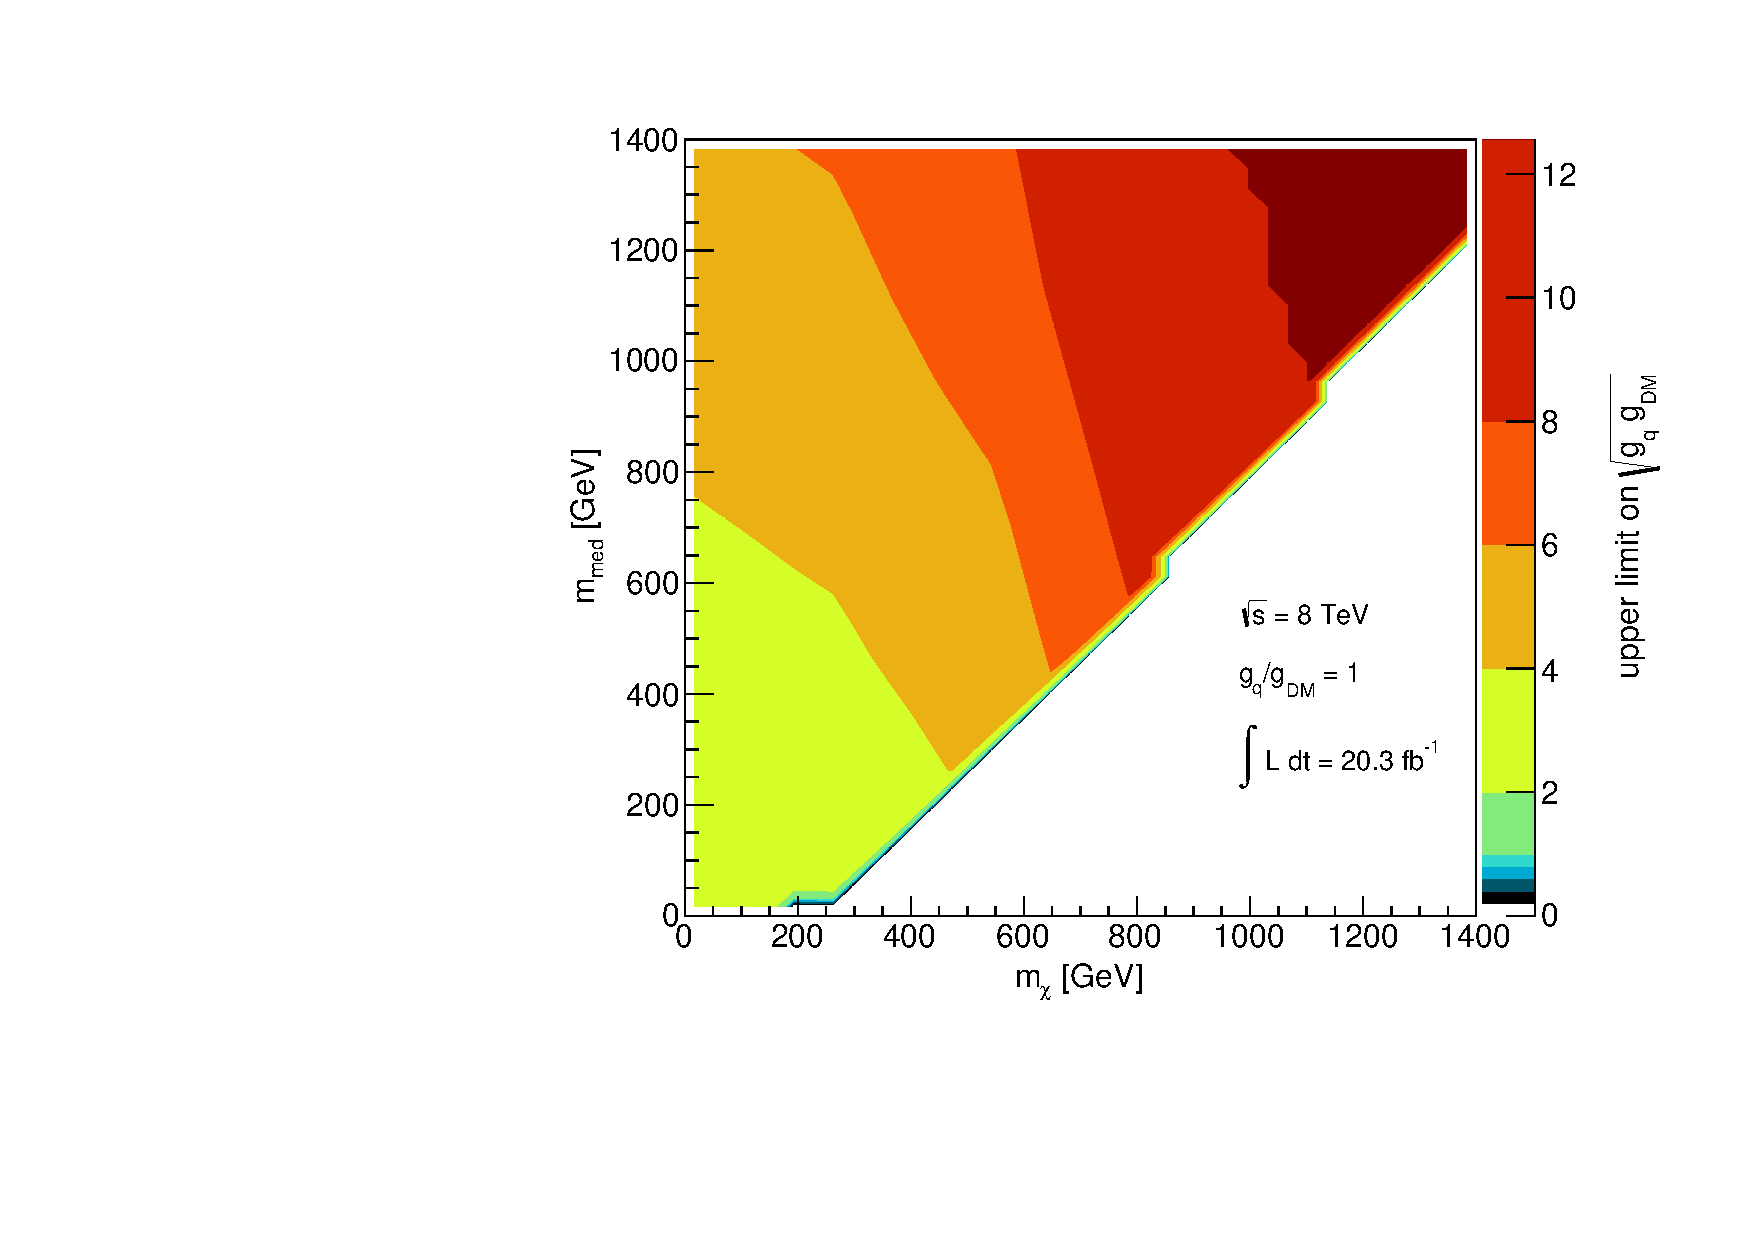
\includegraphics[width=0.45\textwidth]{figures/coupling_limits_TSD_1.pdf}
\caption{sS model coupling limit. REPLACE WITH SS MODEL PLOTS.}
\label{fig:MonoZ_SSD_couplinglimit}
\end{center}
\end{figure}

\begin{figure}[!h]
\begin{center}
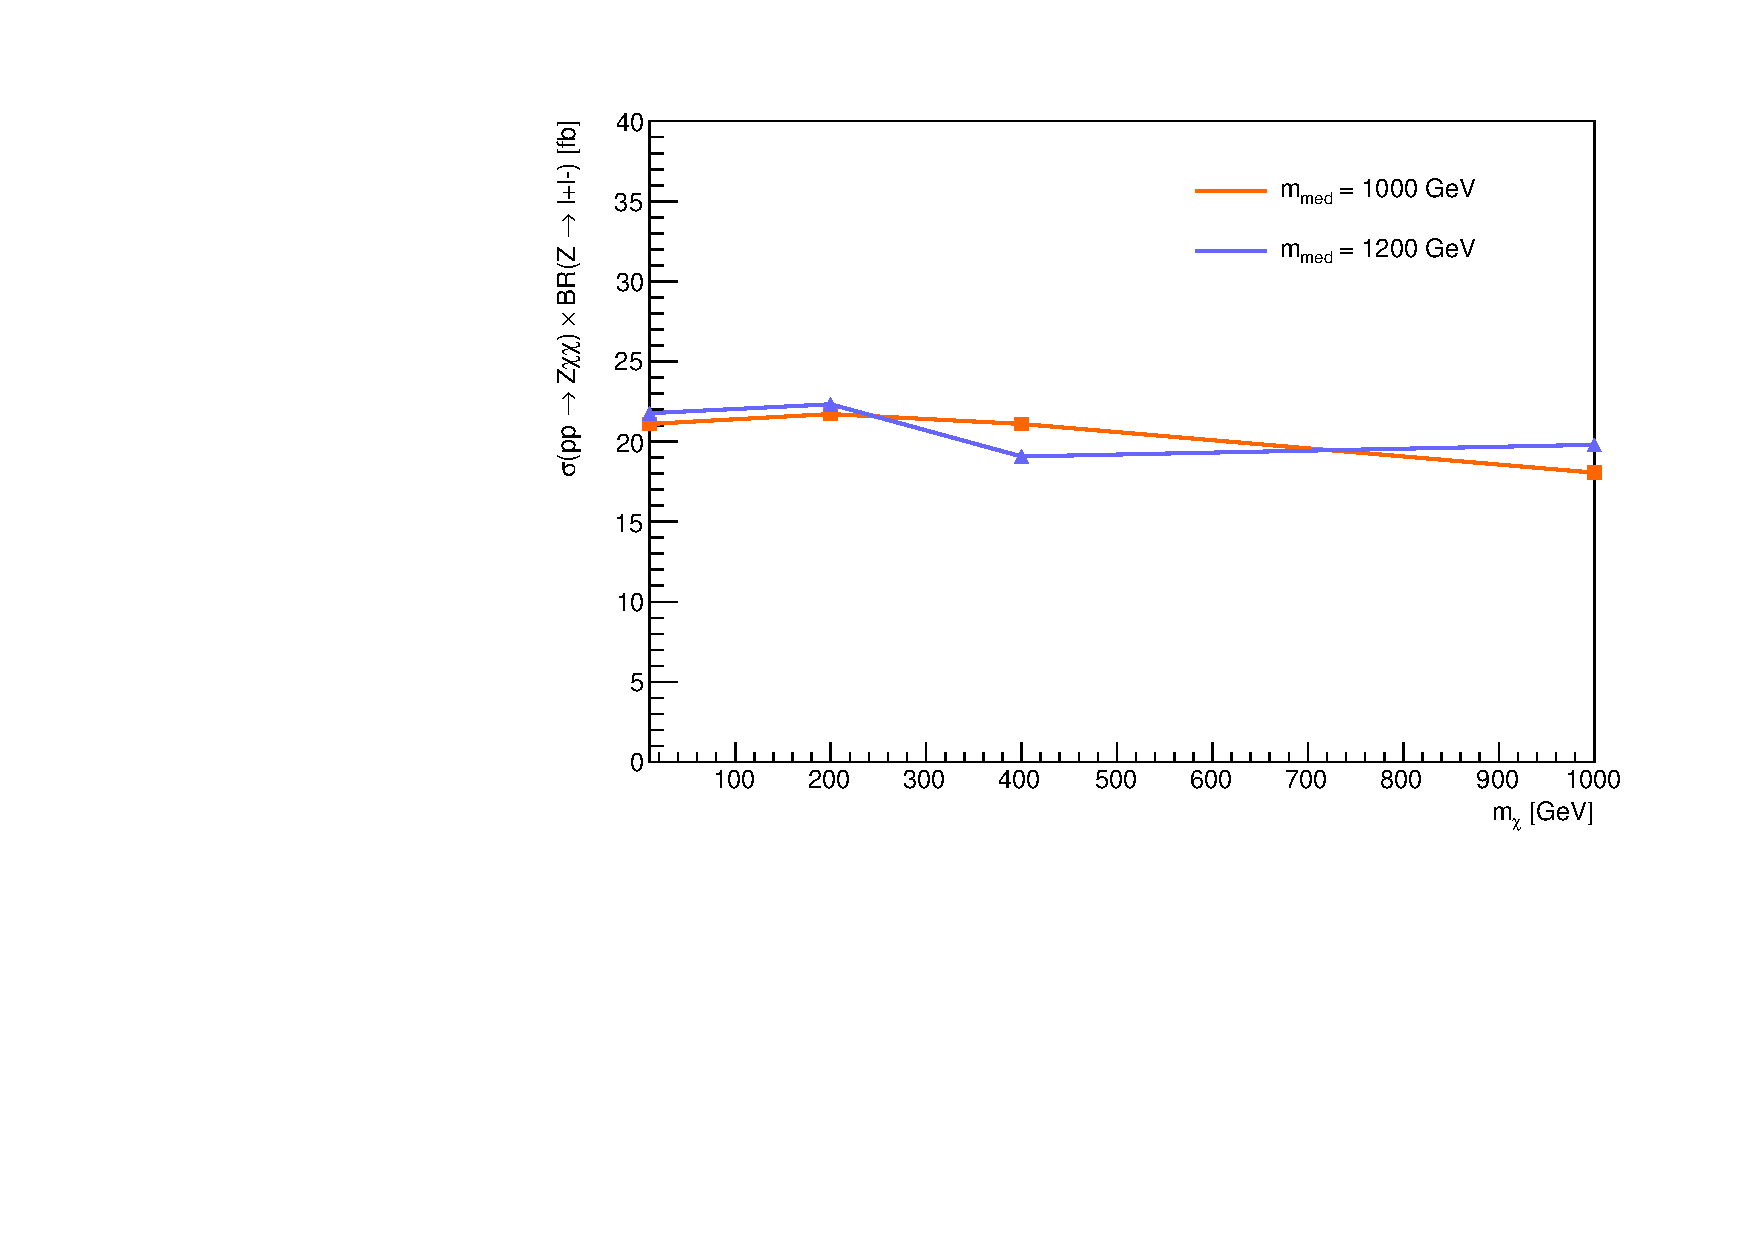
\includegraphics[width=0.45\textwidth]{figures/monoZ_sigma_limits_variedDMmass.pdf}
\caption{Mono-Z channel, tS model. REPLACE WITH TS MODEL PLOTS.}
\label{fig:MonoZ_TSD_limit}
\end{center}
\end{figure}

\begin{figure}[!h]
\begin{center}
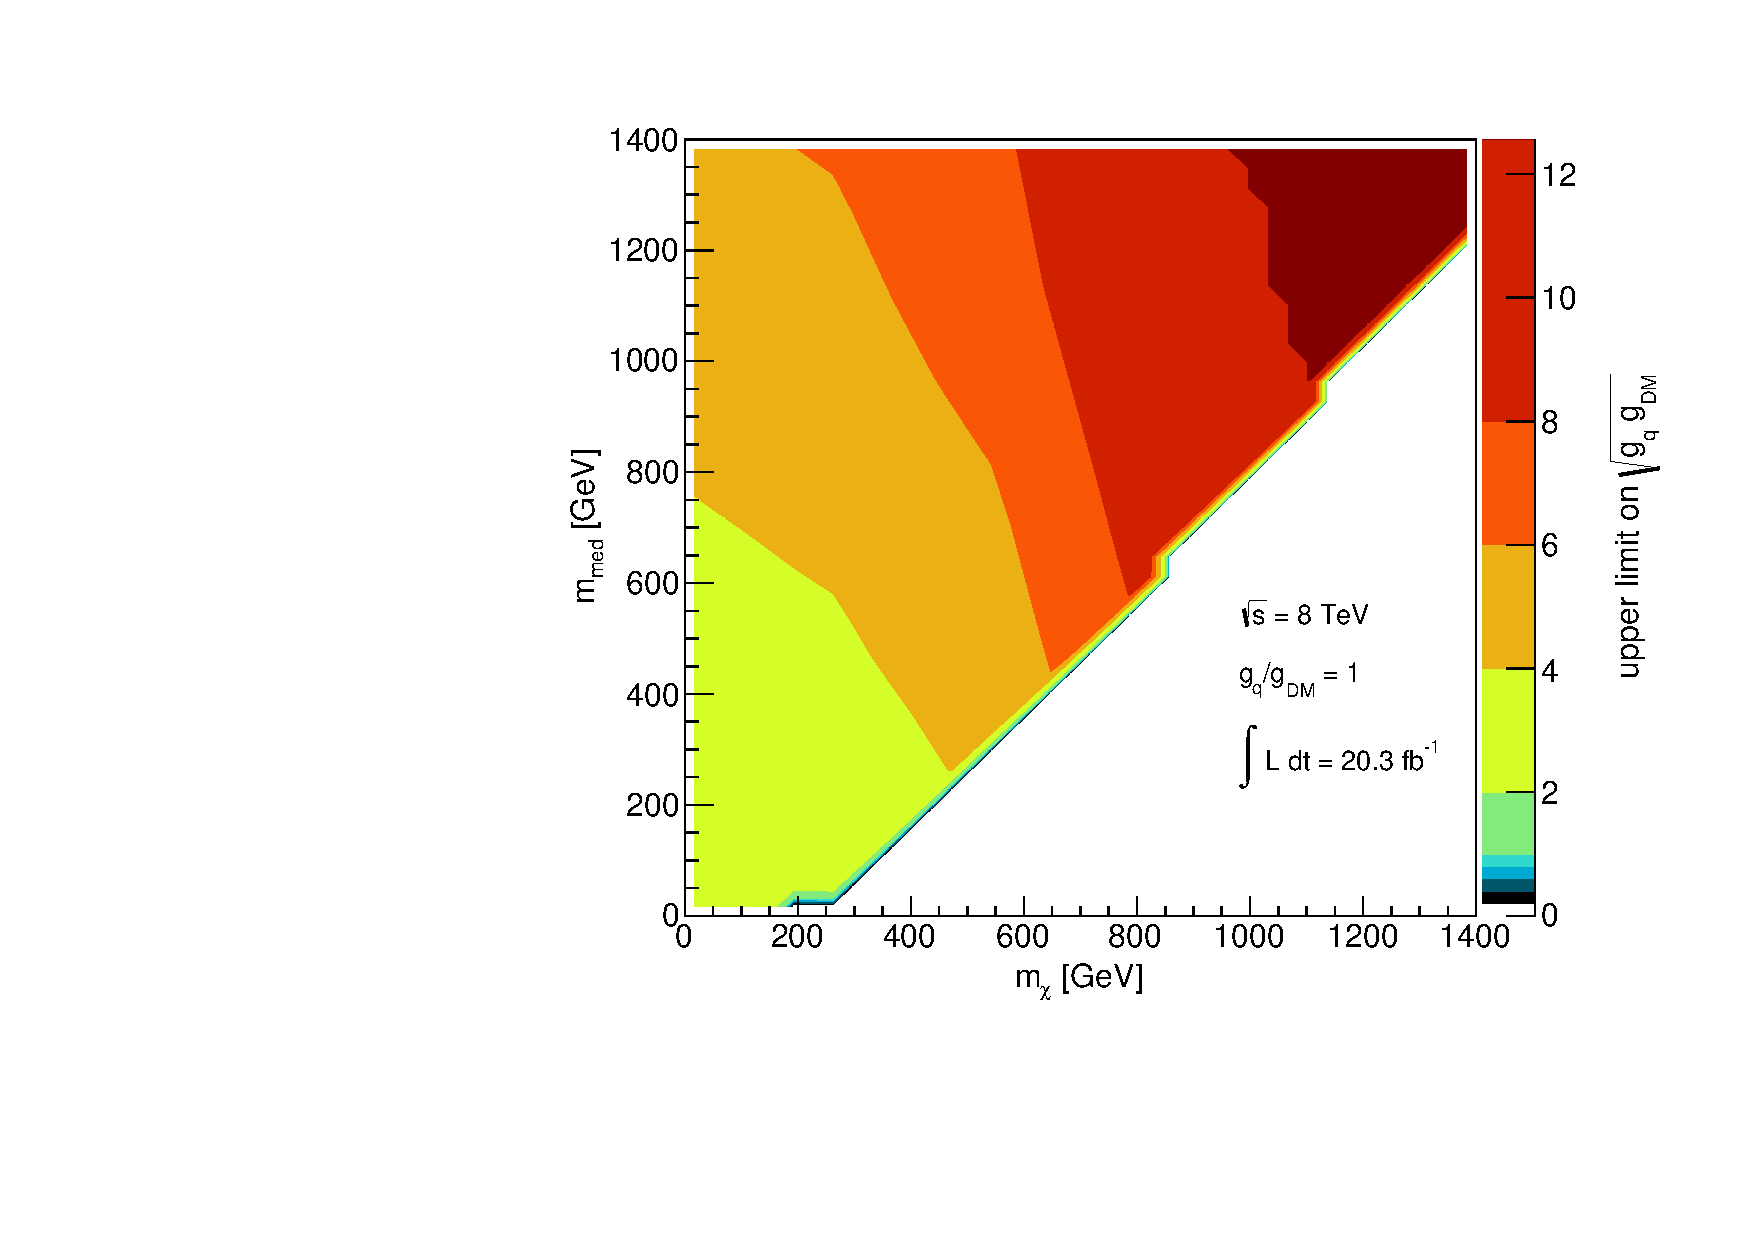
\includegraphics[width=0.45\textwidth]{figures/coupling_limits_TSD_1.pdf}
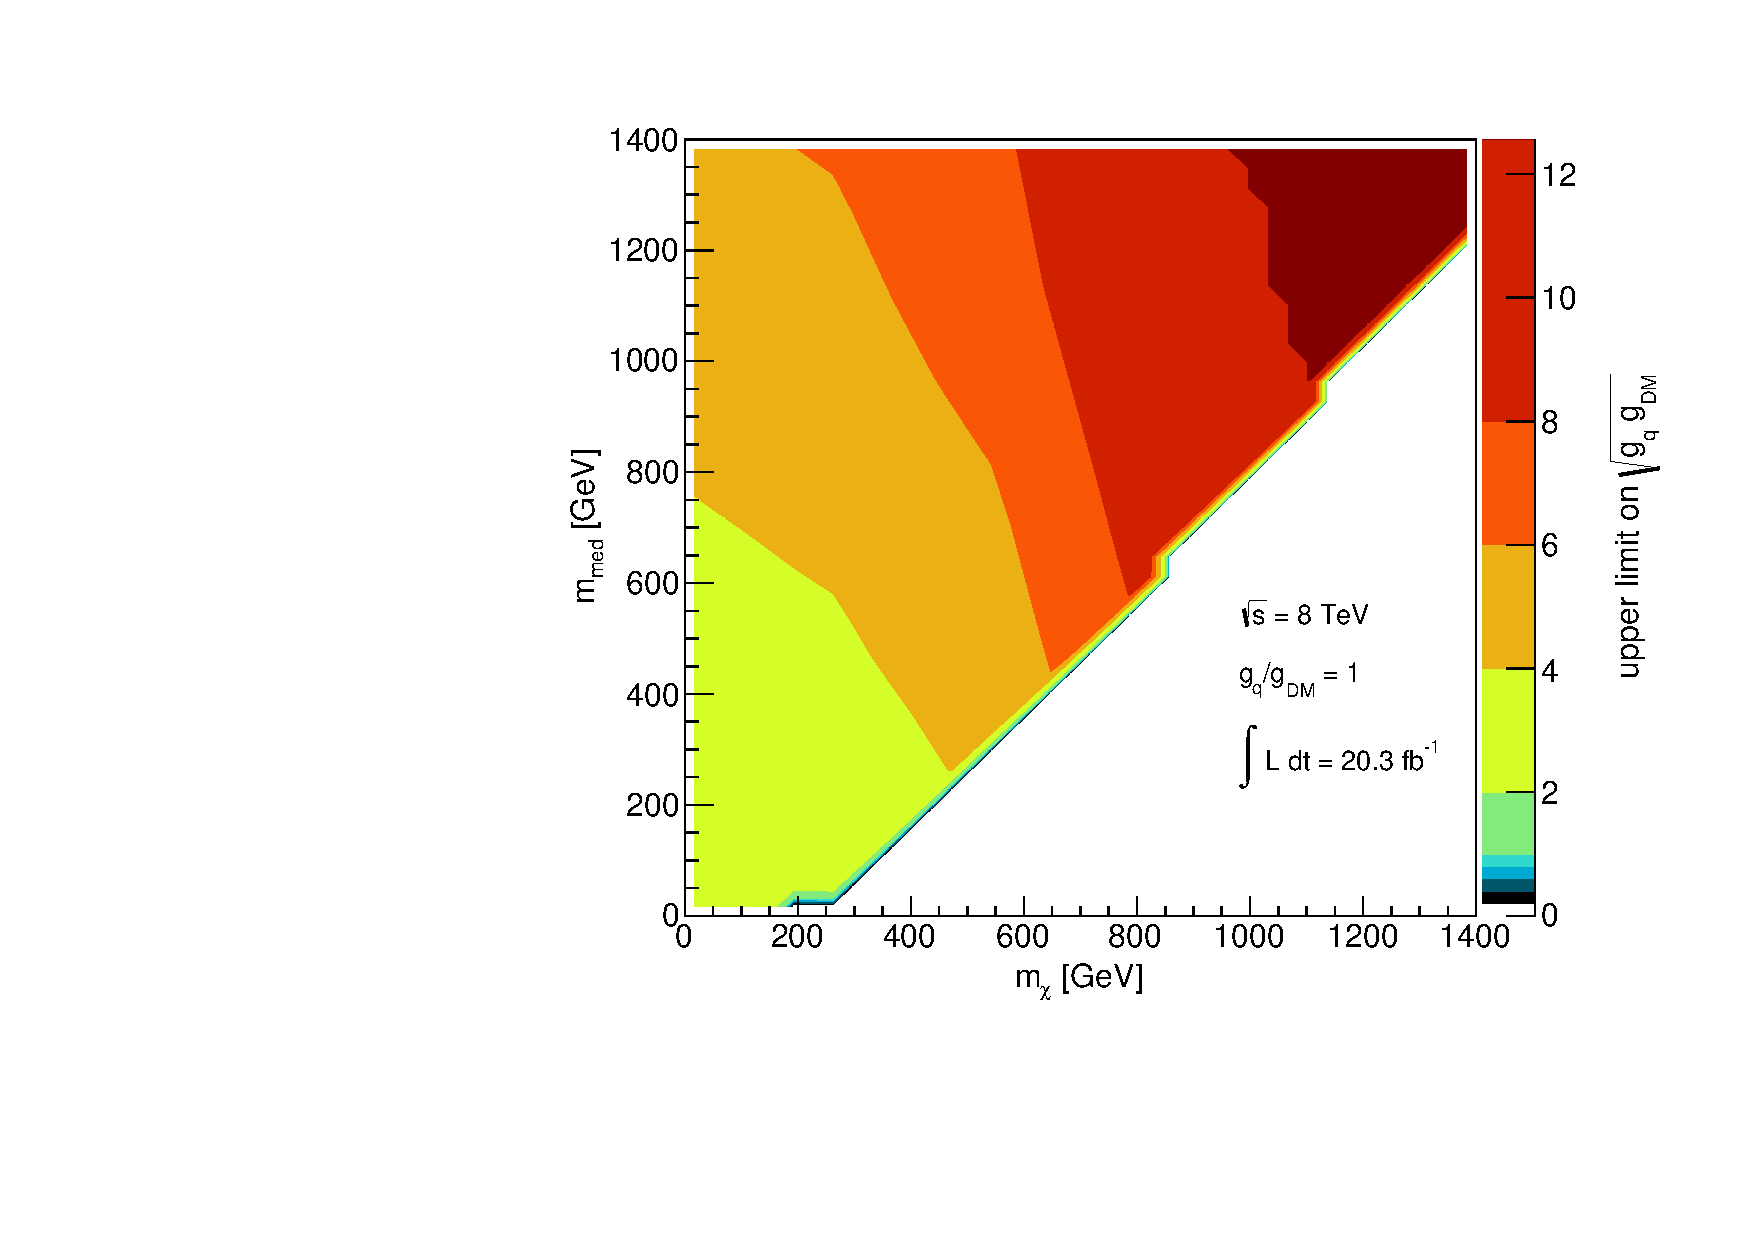
\includegraphics[width=0.45\textwidth]{figures/coupling_limits_TSD_1.pdf}
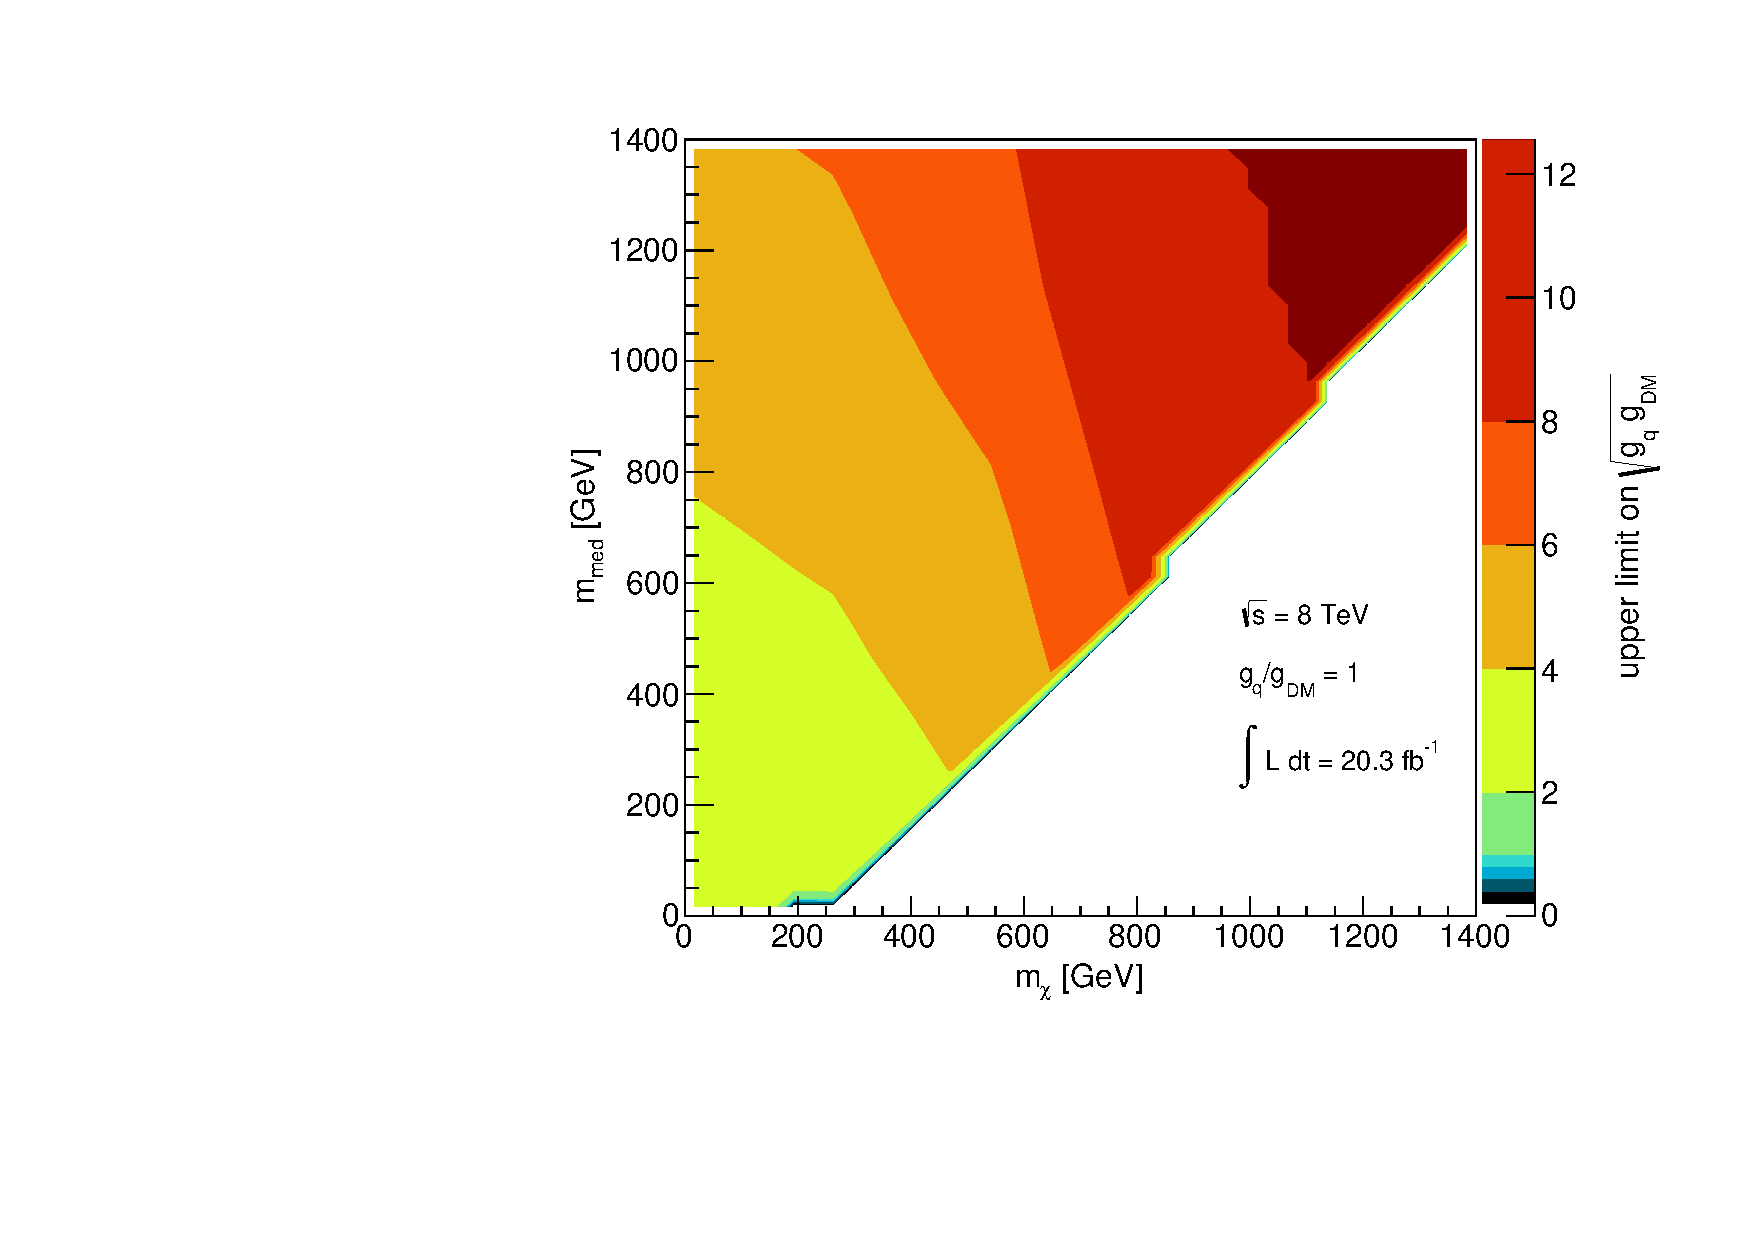
\includegraphics[width=0.45\textwidth]{figures/coupling_limits_TSD_1.pdf}
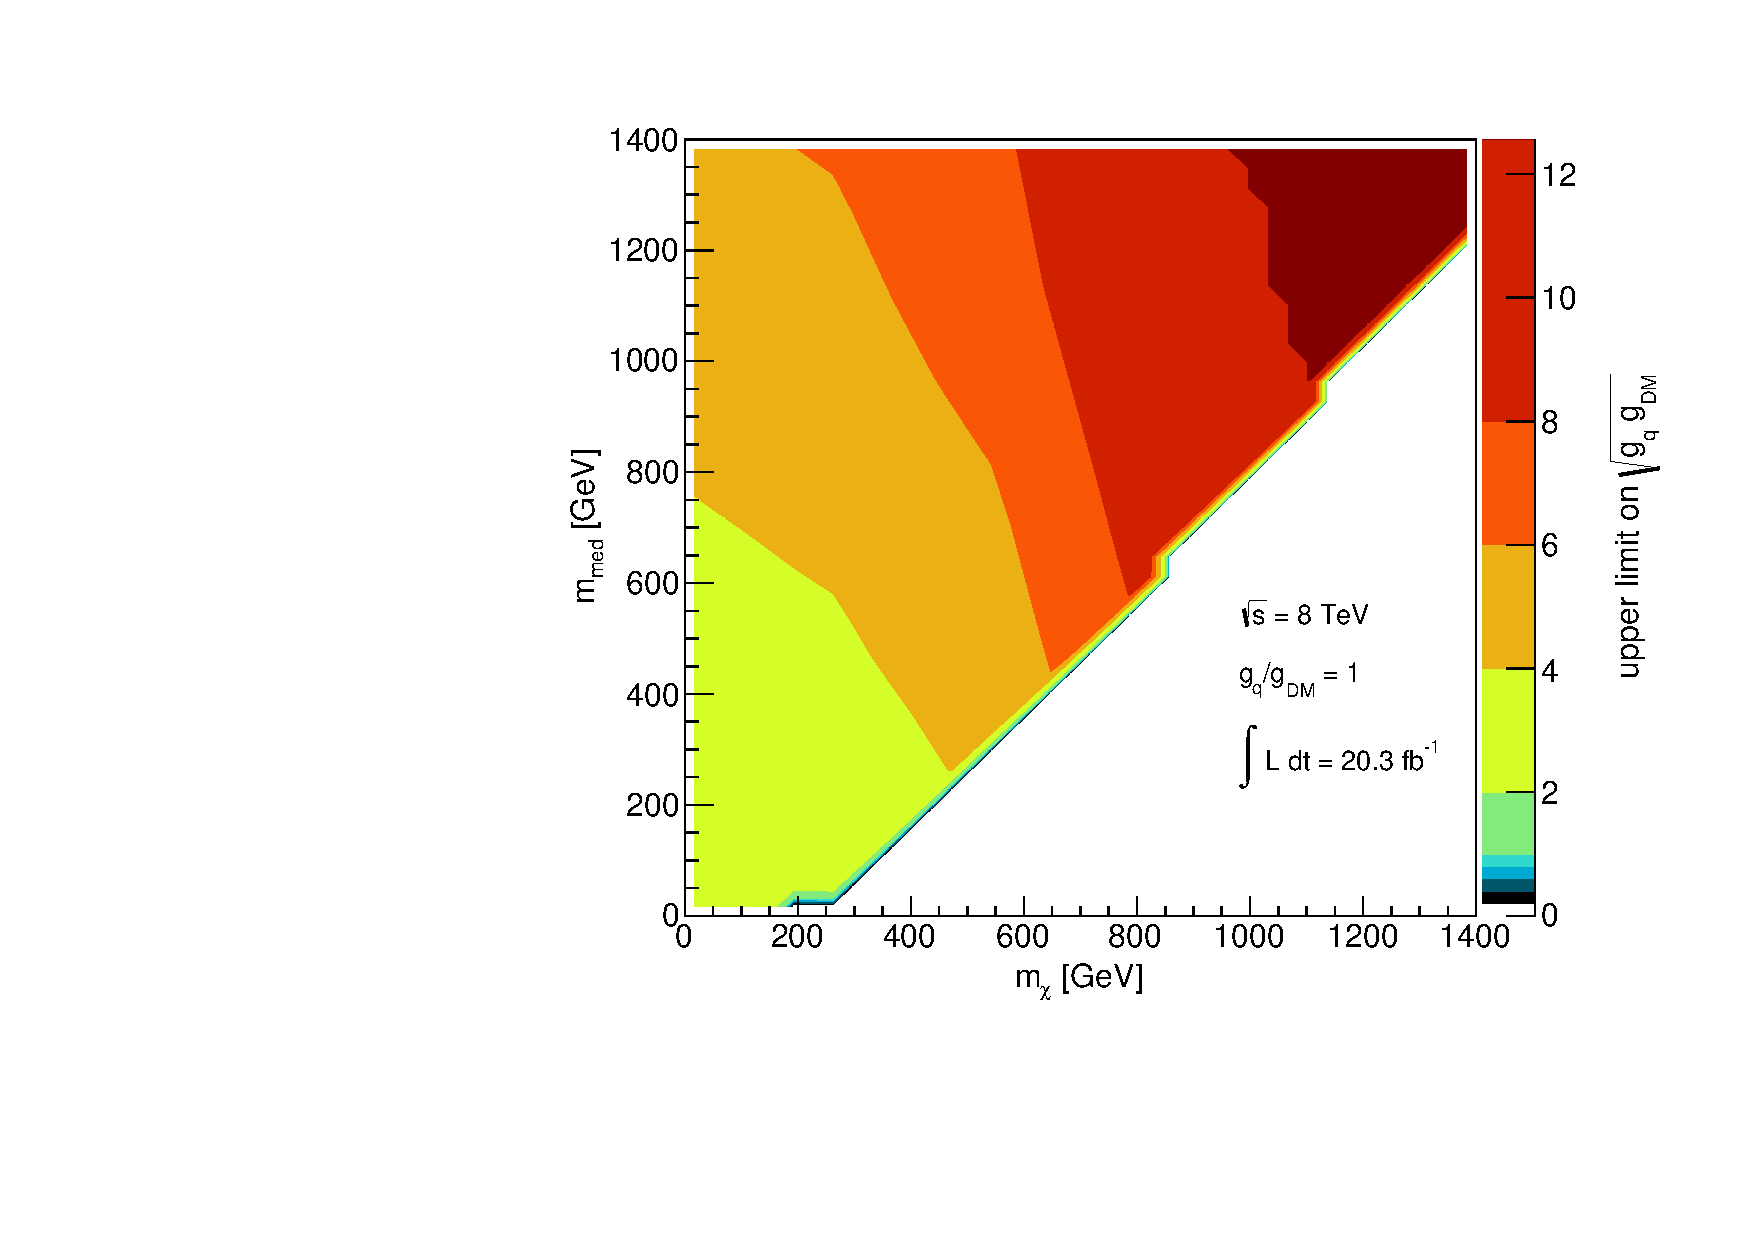
\includegraphics[width=0.45\textwidth]{figures/coupling_limits_TSD_1.pdf}
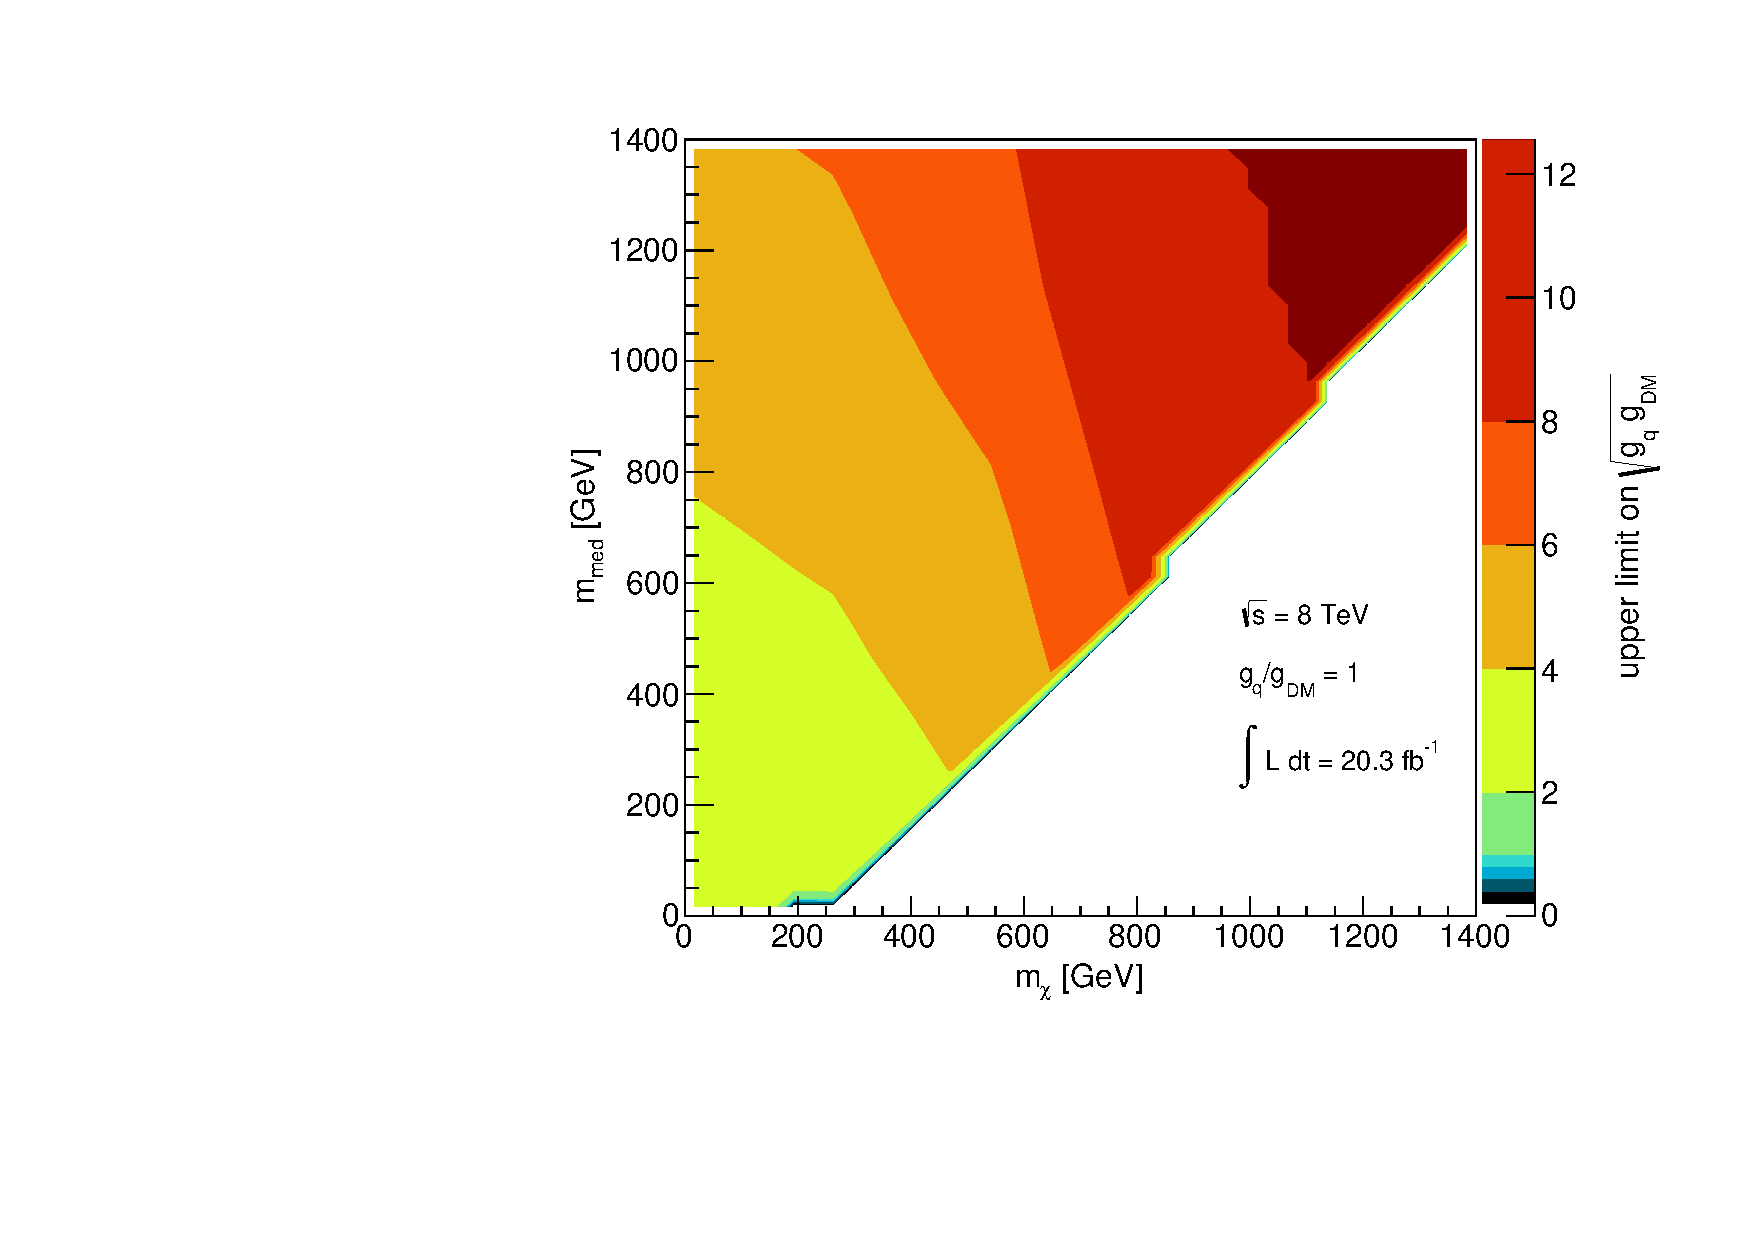
\includegraphics[width=0.45\textwidth]{figures/coupling_limits_TSD_1.pdf}
\caption{tS model coupling limit. REPLACE WITH TS MODEL PLOTS.}
\label{fig:MonoZ_TSD_couplinglimit}
\end{center}
\end{figure}

%%%%%%%%%%%%%%%%%%%%%%%%%%%%%%%%
\subsection{Comparison with Relic Density Constraints}
%%%%%%%%%%%%%%%%%%%%%%%%%%%%%%%%

\comm{Copied from my paper with Karl, so I'll have to rewrite - Tom.}

If dark matter was produced thermally in the early universe, there is a simple relationship between the thermally averaged dark matter self-annihilation cross section $\langle\sigma v\rangle_{\rm ann}$, and the observed relic abundance $\Omega_{\rm DM}h^2$. For a given model, this allows us to find the coupling strength which provides the correct relic abundance as a function of $(m_\chi, M)$. 
%
This scenario is by no means a certainty; If the observed dark matter was produced through some mechanism other than thermal production, or if some new physics has an effect on the connection between the self-annihilation rate and the abundance at freezeout, this relationship breaks down. At the same time, thermal dark matter is a well-motivated scenario, and is a useful way to get a sense of the regions of parameter space within which we expect the gravitationally-observed DM to lie. 

The observed relic abundance can be approximated as
%
\begin{equation}
\Omega_{\rm DM}h^2\simeq \frac{2\times2.4\times 10^{-10}\,{\rm GeV}^{-2}}{\langle\sigma v\rangle_{\rm ann}}.
\label{simplerelic}
\end{equation}
%
Combined with Planck constraints of $\Omega_{\rm DM}^{\rm obs}h^2=0.1199\pm0.0027$ \cite{Ade:2013zuv}, we see that $\langle\sigma v\rangle_{\rm ann}\simeq 4.0\times 10^{-9}\,{\rm GeV}^{-2}$ for thermal relic DM. 
%
We use a more accurate method to constrain $\langle\sigma v\rangle_{\rm ann}$, by simultaneously solving an expression for the freezeout temperature as a function of $\langle\sigma v\rangle_{\rm ann}$, and the relic abundance as a function of both $\langle\sigma v\rangle_{\rm ann}$ and the freezeout temperature. We follow the formalism and technique from Ref.~\cite{Busoni:2014gta}.

We indicate on the figures below a line where the LHC constraint on the coupling strength corresponds to the coupling strength which would give thermal relic DM. In regions \draft{above the line or possibly below} this line, the relic density will naively be too large. For DM to lie in this region, either the thermal relic scenario must break down, or the DM annihilates via additional channels not considered here.
